\documentclass[../master_thesis.tex]{subfiles}
\begin{document}

Our goal is to study the homogeneous magnetostatic problem on the exterior 
of a toroidal Lipschitz domain. That means 
that for the unbounded domain $\Omega \subseteq \real^3$ we have
$\real^3 \setminus \Omega$ is the closure of a toroidal set. 
At the moment, toroidal is a very heuristic term, but we will later specify 
the exact topological assumption for the proof.
We also need a 
piecewise smooth closed curve $\Gamma$ around the torus (see Fig.\,\ref{fig:exterior_domain_with_curve_integral})
because we want to use the curve integral along this $\Gamma$ as an additional 
constraint.

Let $\mathbf{B}$ be the magnetic field. Then we obtain the following problem:
Find a vector field $\mathbf{B}$ on $\Omega$ s.t.
\begin{align}
    \curl \, \mathbf{B} &= 0, \\ 
    \diver \, \mathbf{B}  &= 0 \text{ in } \Omega \\
    \mathbf{B} \cdot \mathbf{n} &= 0 \text{ on } \partial \Omega \text{ and }\label{eq:pointwise_normal_trace}\\ 
    \int_\Gamma \mathbf{B} \cdot d\ell &= C_0 \label{eq:first_curve_integral_condition}
\end{align}
where $\mathbf{n}$ is the outward normal vector field on $\partial \Omega$ and 
$C_0 \in \real$. 


In order to show existence and uniqueness, we first have to find
a proper formulation of this problem. This requires 
appropriate assumptions on the domain $\Omega$ and restating the problem
in terms of the correct Sobolev spaces which will be explained later.

We will first spend a lot of work in introducing the tools needed for the proof.
In Section \ref{sec:differential_forms} will define differential forms with 
all necessary operations on them. Section \ref{sec:singular_homology} is then a very short
overview over the basics of  
singular homology from algebraic topology. This will be needed to properly formulate and treat the
curve integral condition described above. It will culminate in de Rham's theorem 
which can be seen as the connection between differential forms and singular homology.
In Section \ref{sec:hilbert_complexes}, the focus lies on 
unbounded operators and the concept of a Hilbert complex which will be a
fundamental tool in our proofs of existence and uniqueness. At last, we will 
use the developed theory in Section \ref{sec:existence_and_uniqueness} 
to formulate the problem rigorously and proof existence and uniqueness under 
reasonable assumptions. 

Throughout the first chapters, we will provide 
definitions, basic results and show the proofs of many of them if they are not too 
long or trivial. Since all the presented topics are vast these sections should be 
seen as a very basic introduction, but references will be given.

\section{Differential forms}\label{sec:differential_forms}

We will introduce differential forms on manifolds. We start with the abstract 
formulation of alternating forms on finite dimensional real vector spaces 
in Section \ref{sec:alternating_maps}. After a short introduction of 
the essential notions from differential geometry in Section \ref{sec:differential_geometry}
we will finally define differential forms and operations on them 
in Section \ref{sec:differential_forms_subsection}. The integration 
of differential forms will be developed in its own Section \ref{sec:integration_of_differential_forms} 
at the end.

\subsection{Alternating forms} \label{sec:alternating_maps}

Understanding alternating forms is essential in understanding differential forms 
since these provide us with an alternating form at any point of a manifold. 
That is the reason why we will properly introduce the concept in this 
section first.
For the introduction of alternating forms we follow
the short section in Arnold's book
\cite[Sec. 6.1.]{arnold} combine it 
with material from \cite[Sec.\,V.1]{topology_and_geometry}.
However, more arguments and additional details are provided especially  
in Sec.\,\ref{sec:scalar_and_vector_proxies} about scalar and vector proxies.

\subsubsection{Basic definitions}

\begin{definition}[Alternating $k$-linear form]
    Let $V$ be a real vector space with $\text{dim}\,V = n$.
    We call $\omega: V^k \rightarrow \real$ 
    \textit{$k$-linear form} if it is linear in every argument.
    We call a $k$-linear form 
    \textit{alternating} if the sign switches when two arguments are exchanged 
    i.e.
    \begin{align*}
        &\omega(v_1,...,v_i,...,v_j,...,v_k)
        = - \omega(v_1,...,v_j,...,v_i,...,v_k), 
        \\& \quad \text{for } 1\leq i < j \leq k,
        \quad v_1,...,v_k \in V.
    \end{align*}
    We denote the space of alternating $k$-linear forms on $V$ as $\alternating{k}{V}$.
    For the special case $k=0$ we define $\alternating{0}{V} \vcentcolon= \real$.
\end{definition}

Let $\mathcal{S}_k$ be the set of all permutations 
$\{ 1, 2, ..., k\} \rightarrow \{ 1, 2, ..., k \}$. A 
permutation that only exchanges two numbers is called transposition 
and the transposition that exchanges $i$ and $j$ with 
$i \neq j$ is denoted by $(i,j)$. Every permutation can be written as the composition of 
transpositions. This decomposition into transpositions is not unique.
Take a permutation $\pi \in \mathcal{S}_k$ and decompose it into transpositions
\begin{align*}
    \pi = \tau_p \circ \tau_{p-1} \circ ... \circ \tau_1.
\end{align*}
The sign $\sgn(\pi)$ of a permutation 
$\pi: \{ 1,2,...,n\} \rightarrow \{ 1,2, ..., n\}$ is equal to $(-1)^p$.
Even though the decomposition is not unique the parity of the number of
transpositions is always the same and hence the sign is well-defined.
For example, the permutation $(1,2,3,4) \mapsto (2,3,1,4)$ 
can be built by performing the transpositions $(1,2)$ and $(1,3)$ so 
$\sgn(\pi) = (-1)^2 = 1$. 

Going back to alternating forms, this means for any permutation 
$\pi: \{1,2,...,k\} \rightarrow \{1,2,...,k\}$ and 
$\omega \in \alternating{k}{V}$
\begin{align*}
    \omega(v_{\pi(1)},v_{\pi(2)},...,v_{\pi(k)})
    = \sgn(\pi)\, \omega(v_1, v_2,..., v_k).
\end{align*}

\begin{definition}[Wedge product]
    For $\omega \in 
    \alternating{k}{V}$, $\mu \in 
    \alternating{l}{V}$ we define the wedge product $\omega \wedge \mu \in 
    \alternating{k+l}{V}$ 
    \begin{align*}
        &(\omega \wedge \mu) (v_1,...,v_k,v_{k+1},...,v_{k+l}) 
        \\ &= \sum\limits_\pi
        \text{sgn}(\pi)\, \omega(v_{\pi(1)},...,v_{\pi(k)}) \,
        \nu(v_{\pi(k+1)},...,v_{\pi(k+l)})
    \end{align*}
    where we sum over all permutations 
    $\pi \in \mathcal{S}_{k+l}$ 
    s.t. $\pi(1) < ... < \pi(k)$ and $\pi(k+1) < ... < \pi(k+l)$.        
\end{definition}

Let us mention some important properties of the wedge product. It is 
associative, but not commutative. For $\omega \in 
\alternating{k}{V}$, $\mu \in 
\alternating{l}{V}$ we have 
\begin{align}
    \omega \wedge \mu = (-1)^{kl} \mu \wedge \omega. \label{eq:commutativity_wedge_product}
\end{align}
We denote the dual space of $V$ as $V'$.
Recalling the definition of the sign of a permutation $\pi \in \mathcal{S}_k$, 
we get for linear forms $\omega_1, \omega_2, ..., \omega_k \in V'$
\begin{align*}
    \omega_{\pi(1)} \wedge \omega_{\pi(2)} \wedge ... \wedge \omega_{\pi(k)}
    = \sgn(\pi) \, \omega_1 \wedge \omega_2 \wedge ... \wedge \omega_k
\end{align*}
and if a linear form appears twice then the expression is zero.

There is a useful formula for computing the wedge product of linear forms.
For  $\omega_1,...,\omega_k \in \alternating{1}{V} = V'$
, $k \leq n$ we have the formula (\cite[p.260]{topology_and_geometry})
\begin{align}
    \omega_1 \wedge ... \wedge \omega_k (v_1,...,v_k)
    = \det \big( \langle \omega_s, v_t \rangle \big)_{1\leq s,t \leq n}. 
    \label{eq:wedge_product_of_one_forms}
\end{align}
This formula can be easily proven by induction using the definition of the 
wedge product and the determinant.

We will use the dual inner product notation i.e. for $\ell \in V'$ we denote 
\begin{align*}
    \langle \ell, v \rangle_{V' \times V} \vcentcolon= \ell (v)
\end{align*}
and we will usually not write the subscript if it is clear that the dual product is used.
Let $\{ b_i\}_{i=1}^n$ be any basis of $V$ and $\{ b^i\}_{i=1}^n$ the 
correspoding dual basis i.e. 
$b^i \in V'$, $\langle b^i, b_j \rangle = \delta_{ij}$ for $i,j = 1,2,..., n$. Then 
\begin{align*}
    \{b^{i_1} \wedge b^{i_2} \wedge ... \wedge b^{i_k} | \, 
    1 \leq i_1 < ... < i_k \leq n \}
\end{align*}
is a basis of $\alternating{k}{V}$. In particular, 
$\dim\, \alternating{k}{V} = \binom{n}{k}$.

Assume now that we are given an inner product $\langle \cdot, \cdot \rangle_V$ on $V$, 
where we will usually leave out the 
subscript if it is clear what space we mean.
Recall the Riesz isomorphism $\Phi: V \rightarrow V'$ defined by
\begin{align*}
   \langle \Phi v, w \rangle = \langle v, w \rangle.
\end{align*}
Then we obtain an inner 
product on the dual space $V'$ by using the Riesz isomorphism $\Phi$ 
\begin{align*}
    \langle \Phi v, \Phi w \rangle_{V'} \vcentcolon= \langle v, w \rangle_V
\end{align*}
which makes the Riesz isomorphism an isometry.

Now we can define an inner product on $\alternating{k}{V}$ by defining
\begin{align}
    \langle b^{i_1} \wedge b^{i_2} \wedge... \wedge b^{i_k}, 
    b^{j_1} \wedge... \wedge b^{j_k} \rangle_{\alternating{k}{V}} 
    \vcentcolon= \det  \big( \langle b^{i_k}, b^{i_l} \rangle_V \big)_
    {1\leq k,l \leq n} \label{eq:inner_product_alternating_forms}
\end{align}
which is then extended to all of $\alternating{k}{V}$ by linearity. 
We denote with $\lvert \, \cdot\, \rvert _\alternating{k}{V}$ the induced norm.
For an orthonormal basis 
$u_1,...,u_n$ the corresponding basis 
$u^{i_1} \wedge u^{i_2} \wedge ... \wedge u^{i_k}$, 
$1\leq i_1 < ... < i_k \leq n$ is an orthonormal basis of $\alternating{k}{V}$.
Next, we want to introduce the \textit{pullback} as a natural linear
mapping between spaces of alternating forms. 

\begin{definition}
    Let $V$ and $W$ be finite-dimensional real
    vector spaces with ordered bases $(b_i)_{i=1}^n$ and $(c_j)_{j=1}^m$ 
    respectively. We write a basis in round brackets $(\cdot)$ if it is 
    ordered. Let $L \in \mathcal{L}(V,W)$ where $\mathcal{L}(V,W)$ is the 
    space of linear mappings from $V$ to $W$. For $\omega \in \alternating{k}{W}$
    we define the pullback $L^* \omega \in \alternating{k}{V}$ via 
    \begin{align*}
        (L^* \omega)(v_1,...,v_k) = \omega(L\,v_1,...,L\,v_k).
    \end{align*} 
\end{definition}
It is then easy to see that 
$L^*$ is a linear mapping from $\alternating{k}{W}$ to 
$\alternating{k}{V}$
and from the definitions of the wedge product and 
the pullback it is obvious that
\begin{align*}
    L^*(\omega \wedge \nu) = L^*\omega \wedge L^* \nu \quad \forall 
        \omega \in \alternating{k}{W}, \; \nu \in \alternating{l}{W}.
\end{align*}

\begin{proposition}
    Let $A \in \real^{m\times n}$ be the matrix representation of $L$ in the 
    above bases i.e.
    $L\,b_i = \sum_{j=1}^m A_{ji} c_j$. Then we get the basis representation 
    of the pullback 
    \begin{align}
        L^* (c^{j_1} \wedge c^{j_2} \wedge ... \wedge c^{j_k})
        = \sum\limits_{1 \leq i_1 < ... < i_k \leq n} 
            \det A_{(j_1,...,j_k),(i_1,...,i_k)} \,
            b^{i_1} \wedge b^{i_2} \wedge ... \wedge b^{i_k}
        \label{eq:basis_representation_pullback}
    \end{align}
    where $A_{(j_1,...,j_k),(i_1,...,i_k)}$ is the matrix we get 
    by choosing the rows $j_1,...,j_k$  and the columns $i_1$, ... , $i_k$. 
\end{proposition}
\begin{proof}
    Because $\{ b^{i_1}\wedge b^{i_2}\wedge ... \wedge b^{i_k} 
    \mid 1 \leq i_1 < ... < i_k  \leq n \}$ and 
    $\{ c^{j_1}\wedge c^{j_2}\wedge ... \wedge c^{j_k} 
    \mid 1 \leq j_1 < ... < j_k  \leq m \}$ are bases for $\alternating{k}{V}$ 
    and $\alternating{k}{W}$ respectively, we can find $\lambda_{i_1 \cdots i_k} \in \real$ s.t.
    \begin{align}
        L^* (c^{j_1} \wedge c^{j_2} \wedge ... \wedge c^{j_k})
        = \sum\limits_{1 \leq i_1 < ... < i_k \leq n} 
        \lambda_{i_1 \cdots i_k} b^{i_1} \wedge b^{i_2} \wedge ... \wedge b^{i_k}
        \label{eq:basis_representation_pullback_unspecified_coefficents}
    \end{align}

    Now recall the formula for the wedge product of $1$-forms 
    $\nu_i \in \alternating{1}{V} = V'$
    \begin{align*}
        \nu_1 \wedge ... \wedge \nu_k (v_1,...,v_k) = 
        \det \big( \langle \nu_s, v_t \rangle \big)_{1 \leq s,t \leq n}.
    \end{align*}
    Fix now $1 \leq l_1 < ... <  l_k \leq n$. Then we get from this formula
    $b^{i_1} \wedge b^{i_2} \wedge ... \wedge b^{i_k} ( b_{l_1},...,b_{l_k}) = 1$ 
    i.i.f. $(i_1,...,i_k) = (l_1,...,l_k)$. Here it is important to remember that 
    these indices are ordered. Plugging this into 
    (\ref{eq:basis_representation_pullback_unspecified_coefficents}) gives us 
    \begin{align*}
        \lambda_{l_1 \cdots l_k}  &= 
            L^* (c^{j_1} \wedge c^{j_2} \wedge ... \wedge c^{j_k})
            (b_{l_1},...,b_{l_k})
        \\ &= c^{j_1} \wedge c^{j_2} \wedge ... \wedge c^{j_k} 
            (L\,b_{l_1},...,L\,b_{l_k})
        \\ &= \det \Big( \big \langle c^{j_s}, \sum_{r_t = 1}^m A_{r_t,l_t}c_{r_t} \big \rangle 
            \Big)_{1 \leq s,t \leq k}
        \\ &= \det \Big( \sum_{r_t = 1}^m A_{r_t,l_t} \delta_{j_s,r_t}
            \Big)_{1 \leq s,t \leq k}
        \\ &= \det \big( A_{j_s,l_t} \big)_{1 \leq s,t \leq k}
        \\ &= \det A_{(j_1,...,j_k),(l_1,...,l_k)}.
    \end{align*}
\end{proof}


We want to emphasize the special case of the pullback of an alternating $n$-linear form 
with $m = n$. So take $\omega \in \alternating{n}{W}$. Then we know that 
dim$\,\alternating{n}{W} = {n\choose n} = 1$ and so
$\omega = \lambda\, c^1 \wedge ... \wedge c^n$ for some $\lambda \in \real$. 
There only remains one summand in (\ref{eq:basis_representation_pullback}) 
and we obtain for this special case
\begin{align}
    L^* \omega = \lambda \, \det A \, b^1 \wedge ... \wedge b^n
    \label{eq:pullback_alternating_nlinear_map}
\end{align}

We want to examine $\alternating{n}{V}$ a bit closer. 
$\alternating{n}{V}$ is one-dimensional and so we can choose a basis by fixing 
any non-zero element. We want to choose one specific element 
called the \textit{volume form} which will play a crucial role 
when we define integration on a manifold in Sec.\,\ref{sec:integration_of_differential_forms}. 
We also need it to 
define the Hodge star operator below.

The choice of this volume form will depend on the orientation. 
We say that two ordered bases of $V$ 
have the same orientation if the change of basis has positive determinant. 
That divides the ordered bases into two classes with different orientation.
We choose one of these classes and call these bases positively
oriented. In $\real^n$, the convention is to define the class as 
positively oriented which includes the standard orthonormal basis.

\begin{definition}[Volume form]
    Let $(b_i )_{i=1}^n$ be any positively oriented
    basis. Let $G$ be the Gramian matrix i.e. $G_{ij} = \langle b_i, b_j \rangle$ 
    which is always a symmetric positive definite matrix.
    Then we define the \textit{volume form}
    \begin{align*}
        \vol \vcentcolon= \sqrt{\det G} \, b^1 \wedge b^2 \wedge ... \wedge b^n.
    \end{align*}
\end{definition}

We have the following defining property of the volume form.

\begin{proposition}
    For any ordered
    orthonormal basis $(u_i)_{i=1}^n$ we have 
    \begin{align*}
        \vol (u_1,\,u_2,...,\,u_n) = (-1)^s.
    \end{align*}
    with $s=0$ if $(u_1,...,u_n)$ has the same orientation as $(b_i)_{i=1}^n$ 
    and $s=1$ otherwise. 
\end{proposition}
\begin{proof}
    Let us define the matrix $B \in \real^{n\times n}$, $B_{k,i} = \langle b_i, u_k
    \rangle_V$ which is just the change of basis matrix from $( b_i )_{i=1}^n$ 
    to $( u_i )_{i=1}^n$. 
    Then using basic linear algebra we get
    $ G = B^\top B$ and 
    $\sqrt{\det G} = (-1)^s \det B$. Let now $\Psi$ be the linear map with 
    $\Psi b_i = u_i$. In the basis $( b_i )_{i=1}^n$ this has the matrix 
    representation $B^{-1}$ and so by using 
    (\ref{eq:pullback_alternating_nlinear_map}) we get
    \begin{align*}
        \vol (u_1,\,u_2,...,\,u_n) &= \sqrt{ \det G} \, b^1 \wedge ... \wedge b^n 
        ( \Psi b_1,..., \Psi b_n )
        \\ &= (-1)^s \det B \, \Psi^* (b^1 \wedge ... \wedge b^n )( b_1,..., b_n) 
        \\ &= (-1)^s \det B \, \det B^{-1} \, (b^1 \wedge ... \wedge b^n )( b_1,..., b_n)
        = (-1)^s.
    \end{align*}
\end{proof}
This property also defines the volume form uniquely so it is independent of the 
chosen basis. It only depends on the orientation.
It also shows that $\vol$ is non-zero and thus 
\begin{align*}
    \alternating{n}{V} = \text{span} \{ \vol \}.
\end{align*}

Note that if we choose $\{ b_i \}_{i}$ to be an orthonormal basis to begin 
with the Gramian matrix is just the identity and 
$\vol = b^1 \wedge ... \wedge b^n$. Especially in the case of $\real^n$ if 
we denote the standard basis by $\{ e_i \}_{i=1}^n$ and the resulting 
dual basis as $\{ e^i \}_{i=1}^n$ then 
\begin{align*}
    \vol = e^1 \wedge ... \wedge e^n.
\end{align*}

We will from now on assume that we fixed an orientation on $V$ and with it 
the volume form vol. 
Using the resulting volume form on $V$
we can now define the \textit{Hodge star operator} with the following 
proposition.
\begin{proposition}
    There exists an isomorphism $\star: \alternating{k}{V} 
    \rightarrow \alternating{n-k}{V}$ s.t. 
    \begin{align}
        \omega \wedge \mu = \langle \star \omega, \mu \rangle_{\alternating{n-k}{V}}
        \vol \quad \forall \mu \in \alternating{n-k}{V}.
        \label{eq:hodge_star_definition}            
    \end{align}
    We call this isomorphism the \textit{Hodge star operator}.
\end{proposition}
\begin{proof}

    Let us define $\vol' \in (\alternating{n}{V})'$ via 
    \begin{align*}
        \langle \vol', \vol \rangle = 1.
    \end{align*}
    Recall that $\alternating{n}{V}$ is one-dimensional and so this defines $\vol'$ 
    uniquely. Let us fix $\omega \in \alternating{k}{V}$. 
    Then we take the following linear form on $
    \alternating{n-k}{V}$
    \begin{align*}
        \mu \mapsto \langle \vol' ,\omega \wedge \mu \rangle.
    \end{align*}
    and define
    $\star \omega$ as the Riesz representative of this linear form that means we 
    have $\langle \vol', \omega \wedge \mu \rangle = 
    \langle \star \omega, \mu \rangle_{\alternating{n-k}{V}}$ for all 
    $\mu \in \alternating{n-k}{V}$ which is equivalent to (\ref{eq:hodge_star_definition}).
    Checking linearity is trivial and will be omitted.

    It is also clear from the uniqueness of the Riesz representative that 
    $\star\omega$ is uniquely determined by the above condition and 
    thus $\star$ is injective. Since $\dim \alternating{k}{V} = 
    \binom{n}{k} = \binom{n}{n-k} = \dim \alternating{n-k}{V}$ the injectivity 
    implies surjectivity and $\star$ is an isomorphism.
\end{proof}

Let us collect some important properties of the Hodge star operator.
\begin{proposition}\label{prop:properties_hodge_star}
    Let $(u_i)_{i=1}^n$ be an ordered orthonormal basis of $V$. Let 
    $\{ i_1, ..., i_n \} = \{ 1, ..., n\}$, $i_1 < i_2 < ... < i_k$ and 
    $i_{k+1} < ... < i_n$. Then
    \begin{align}
        \star (u^{i_1} \wedge u^{i_2} \wedge ... \wedge u^{i_k})
        = \sgn(i_1,i_2,...,i_n) \, u^{i_{k+1}} \wedge ... \wedge u^{i_{n}}
        \label{eq:hodge_star_orthonormal_basis}
    \end{align}
    where $\sgn(i_1,i_2,...,i_n)$ 
    is the sign of the permutation $j \mapsto i_j$. In particular, 
    $\star$ is an isometry since it maps orthonormal bases to orthonormal 
    bases. Furthermore,
    \begin{alignat*}{3}
        &\text{(i)} &\quad\star \star \omega = (-1)^{k(n-k)} \omega \quad &\forall \omega 
            \in \alternating{k}{V}\\
        &\text{(ii)} &\quad\omega \wedge \star \nu = \langle \omega, \nu \rangle
            _{\alternating{k}{V}}  \, \vol \quad &\forall \omega, \nu \in \alternating{k}{V}.     
    \end{alignat*}
\end{proposition}
\begin{proof}
    Take $u^{j_{k+1}} \wedge ... \wedge u^{j_n}$ with 
    $1 \leq j_{k+1} < ... < j_n \leq n$. Then 
    \begin{align*}
        &\langle \sgn(i_1,i_2,...,i_n) \, u^{i_{k+1}} \wedge ... \wedge u^{i_{n}},
            u^{j_{k+1}} \wedge ... \wedge u^{j_{n}} \rangle_{\alternating{n-k}{V}}
        \\ &= \sgn(i_1,i_2,...,i_n) \det \big( \langle u^{i_s}, u^{j_t} \rangle \big)_{k+1 \leq s,t \leq n}
        \\ &= \sgn(i_1,i_2,...,i_n) \det \big( \delta_{i_s,j_t} \big)_{k+1 \leq s,t \leq n}.
    \end{align*}
    In the last step we used the fact that $u^i$ are orthonormal since the $u_i$ 
    are. Now observe due to the ordering that 
    $\det \big( \delta_{i_s,j_t} \big)_{k+1 \leq s,t \leq n} = 1$ i.i.f.
    $i_s = j_s$ for $s = k+1,...,n$ and is zero otherwise.

    For the wedge product we get
    \begin{align*}
        u^{i_1} \wedge ... \wedge u^{i_{k}} \wedge u^{j_{k+1}} \wedge ... 
            \wedge u^{j_n}
        =   \begin{cases}
                \sgn(i_1, ..., i_n)\, \vol, & \text{if $(i_{k+1},...,i_n) = (j_{k+1},...,j_n)$} \\
                0,  & \text{otherwise.}
            \end{cases}.
    \end{align*}
    Comparing both expressions we just proved
    \begin{align*}
        &u^{i_1} \wedge ... \wedge u^{i_{k}} \wedge u^{j_{k+1}} \wedge ... \wedge u^{j_n}
        \\ &= \langle \sgn(i_1,i_2,...,i_n) u^{i_{k+1}} \wedge ... \wedge u^{i_{n}},
            u^{j_{k+1}} \wedge ... \wedge u^{j_{n}} \rangle_{\alternating{n-k}{V}} \vol.
    \end{align*}
    Because the $u^{j_{k+1}} \wedge ... \wedge u^{j_n}$ for $j_{k+1} < ... < j_n$ are a 
    basis of $\alternating{n-k}{V}$ we can deduce that 
    \begin{align*}
        u^{i_1} \wedge ... \wedge u^{i_{k}} \wedge \nu = \langle \sgn(i_1,i_2,...,i_n)\, u^{i_{k+1}} \wedge 
        ... \wedge u^{i_{n}}, \nu \rangle_{\alternating{n-k}{V}} \vol.
    \end{align*}
    and thus  
    $\star (u^{i_1} \wedge ... \wedge u^{i_{k}}) = 
    \sgn(i_1,i_2,...,i_n)\, u^{i_{k+1}} \wedge ... \wedge u^{i_{n}}$ as claimed.
    We see from this that $\star$ maps the orthonormal basis of $\alternating{k}{V}$ 
    to an orthonormal
    basis of $\alternating{n-k}{V}$ and is thus an isometry.

    The other two claims follow from that easily. For any $\omega \in 
    \alternating{k}{V}$, $\mu \in \alternating{n-k}{V}$
    \begin{align*}
        \langle \star \star \omega , \mu \rangle_{\alternating{k}{V}}\vol
        &= \star \omega \wedge \mu
        = (-1)^{k(n-k)} \mu \wedge \star \omega 
        \\ &= (-1)^{k(n-k)} \langle \star \mu , \star \omega \rangle_{\alternating{n-k}{V}} \vol
        \\ &= \langle (-1)^{k(n-k)} \omega , \mu \rangle_{\alternating{k}{V}} \vol.
    \end{align*}
    Then the first claim follows since $\mu \in \alternating{k}{V}$ was
    arbitrary.

    For the second claim, take $\omega, \nu \in \alternating{k}{V}$, then
    \begin{align*}
        \omega \wedge \star \nu = \langle \star \nu , \star \omega \rangle _{\alternating{n-k}{V}} \vol
        = \langle \omega , \nu \rangle _{\alternating{k}{V}} \vol.
    \end{align*}
\end{proof}
In particular in $\real^3$, we have 
$\star\star = \text{Id}$. Notice also 
that we always have $\star 1 = \vol$.

Let us quickly derive the expression in any basis 
for the Hodge star applied to linear 
forms which we will need later. Let $\omega = \sum_i \omega_i b^i \in 
\alternating{1}{V} = V'$. Let us denote $g^{ij} = \langle b^i, b^j \rangle$ 
and $G_{ij} = \langle b_i, b_j \rangle$ again the Gramian matrix.
Then we claim
\begin{align}
    \star \omega = \sqrt{\det G} \sum_{i,j=1}^n \omega_i (-1)^{j-1} 
        g^{ij} b^1 \wedge
        b^2 \wedge ... \wedge \widehat{b^j}\wedge ... \wedge b^n 
        \label{eq:hodge_star_one_forms}
\end{align}
where $\widehat{b^j}$ means that it is left out. The proof is very 
simple in this case. Let $\nu$ denote the expression on the right hand side 
of (\ref{eq:hodge_star_one_forms}).
For any $1 \leq l \leq n$ we get
\begin{align*}
    \nu \wedge b^l &= \left( \sqrt{\det G} \sum_{i,j=1}^n \omega_i (-1)^{j-1} g^{ij} b^1 \wedge
        b^2 \wedge ... \wedge \widehat{b^j} \wedge ... \wedge b^n\right) \wedge b^l 
    \\ &= \sqrt{\det G} \sum_{j=1}^n \langle b^j,\sum_{i=1}^n \omega_i  b^i\rangle
        (-1)^{j-1}  b^1 \wedge
        b^2 \wedge ... \wedge \widehat{b^j} \wedge ... \wedge b^n \wedge b^l
    \\ &= \sqrt{\det G} \langle b^l,\omega \rangle
        (-1)^{(l-1)}(-1)^{(n-l)}  b^1 \wedge
        b^2 \wedge ... \wedge b^l  \wedge ... \wedge b^n 
    \\ &= \langle (-1)^{n-1}\omega, b^l \rangle \vol.
\end{align*}
where the inner product is always in the corresponding space of alternating forms.
In the second step, we used that if $j\neq l$ then one basis element must 
appear twice in the wedge product which is then zero. If $j=l$ then 
$\sgn (1,2, ..., \hat{l},...,n,l) = (-1)^{n-l}$ because we need $(n-l)$
transpostions to bring the indices into order. So we proved 
$(-1)^{n-1}\omega = \star \nu$ and thus $\star \omega = (-1)^{n-1} \star\star\nu = \nu$.
This shows also that the explicit expression of the Hodge star becomes much more 
complicated if the basis is not orthonormal.


\subsubsection{Scalar and Vector proxies} \label{sec:scalar_and_vector_proxies}
Now we want to relate alternating maps to elements of the 
vector space $V$ itself or to scalars. Let us start with the easiest 
case. $\alternating{0}{V}$ are already scalars by definition. Now we can use 
the Hodge star operator which is an isometry 
$\star: \alternating{0}{V} \rightarrow \alternating{n}{V}$ with
$\star c = c \vol$. 
For $\omega = \lambda \vol \in \alternating{n}{V}$ we call then
$\star^{-1} \omega = \lambda \in \real$ the \textit{scalar proxy} of $\omega$.

Next, we will move on to $\alternating{1}{V}$ and $\alternating{n-1}{V}$. 
Let $\Phi: V \rightarrow V'$ denote the Riesz isomorphism which is an isometry.
Because $V' = \alternating{1}{V}$ this gives us the correspondence of 
vectors and linear forms. Now we can once again use the Hodge star and obtain 
the isometry $\star \Phi: V \rightarrow \alternating{n-1}{V}$ to find the connection 
between vectors and $(n-1)$-forms. 
For $\omega \in \alternating{1}{V} = V'$ we then call 
$\Phi^{-1} \omega \in V$ the \textit{vector proxy} of $\omega$.
For $\nu \in \alternating{n-1}{V}$ the vector proxy is 
$\Phi^{-1} \star^{-1} \nu \in V$.

These ways to identify alternating forms gives us the 
ability to look at the notions defined above in the context of scalars 
and vectors.
Let us look at the wedge product. We have for $v,w \in V$
\begin{align*}
    \Phi v \wedge \star \Phi w = \langle \Phi v , \Phi w \rangle_{V'} \vol
    = \langle v , w \rangle_{V} \vol
\end{align*}
which means that the wedge product of a linear form and an alternating $(n-1)$-
linear form corresponds in proxies to the inner product.

In the case of $V= \real^3$ with the standard basis
vectors $e_1$, $e_2$ and $e_3$ denote the resulting elements 
of the dual basis with $e^1$, $e^2$ and $e^3$ respectively. 
Take $v = v_1 e_1 + v_2 e_2 + v_3 e_3 \in \real^3$ 
and recall that for a orthonormal basis the Riesz isomorphism maps basis 
elements to their dual basis elements i.e. $\Phi e_i = e^i$. Hence, 
we get $\Phi v = v_1 e^1 + v_2 e^2 + v_3 e^3$. Take another $w \in \real^3$.
Then using the $e^i \wedge e^j = - e^j \wedge e^i$ we get 
\begin{align}
    \Phi v \wedge \Phi w = \star \Phi (v \times w). 
    \label{eq:cross_product_as_wedge_product}
\end{align}
That means in $3D$ in terms of vector proxies, the wedge product 
of two linear forms corresponds to the cross product. Note that 
(\ref{eq:cross_product_as_wedge_product}) is formulated without using a 
specific basis and can therefore be computed using any basis i.e. 
if we have $v = \tilde{v}_1 b_1 + \tilde{v}_2 b_2 + \tilde{v}_3 b_3$ 
and analogous for $w$ we could still calculate the cross product directly as 
\begin{align*}
    v \times w = \Phi^{-1} \star \big(\Phi v \wedge \Phi w \big).
\end{align*}
One has to take care though because if the basis is not orthonormal 
the Riesz isomorphism does not map basis elements $b_i$ to their respective 
dual basis elements $b^i$. Instead we have 
\begin{align*}
    \Phi b_i = \sum_{i=1}^{n} \langle b_j, b_i \rangle b^j
\end{align*}
i.e. it has the Gramian matrix $G$ as basis representation. 
This is easy to 
see. Let $\Phi b_i = \sum_j \lambda_j b^j$. Then
\begin{align*}
    \lambda_j = \langle \Phi b_i ,b_j \rangle = \langle b_i, b_j \rangle.
\end{align*}
As derived above, the Hodge star is not as trivial to compute either.

Similarly, we want to explore the pullback in terms of vector proxies as well. 
These will be important in the next section when we talk about the pullback 
of differential forms and apply these to the tranformation of integrals.
In order to avoid complicated computations we will stick to orthonormal bases.
Let $\{ b_i \}_{i=1}^n$ be an orthonormal basis of $V$ and 
$\{ c_j \}_{j=1}^m$ be an orthonormal basis of $W$. Let $L : V \rightarrow W$ 
again be a linear map and $A$ be the basis representation of it w.r.t. 
the two bases given i.e. $L b_i = \sum_j A_{ji} c_j$. 
Then we get the pullback of linear forms in terms 
of vector proxies 
as $\Phi_V^{-1} L^* \Phi_W : W \rightarrow V$. Recall 
formula (\ref{eq:pullback_alternating_nlinear_map}) which 
gives us for the pullback of one forms 
\begin{align}
    L^* c^j = \sum_{i=1}^n A_{j,i} b^i \label{eq:pullback_linear_forms}
\end{align}
so the matrix representation w.r.t. the given dual bases is $A^\top$.
Then since we have $\Phi_V b_i = b^i$ and analogous for $c^j$
the matrix representation of the Riesz isomorphism is just the identity.
In total, the basis representation of $\Phi_V^{-1} L^* \Phi_W$ is 
$A^\top$.

For $m=n$ let us look at the pullback of alternating $(n-1)$-linear maps.
In terms of vector proxies this can then be expressed as 
$\Phi_V^{-1} \star^{-1} L^* \star \Phi_W$. Note that we used the same symbol 
$\star$, but it is once applied in $W$ and then the inverse in $V$. It 
can be shown with the same ideas and (\ref{eq:hodge_star_orthonormal_basis})
that the matrix representation is the adjugate matrix 
$\text{ad}(A)$ defined as 
\begin{align*}
    \text{ad}(A)_{ij} = (-1)^{i+j} \det A_{-j,-i}
\end{align*} 
where $A_{-j,-i}$ is the matrix without the $j$-th row and $i$-th column.
If $A$ is invertible then $(\det A)\,A^{-1} =  \text{ad}(A)$. 

The pullback of $n$-linear alternating forms in terms of scalar proxies is 
$\star^{-1} L^* \star$. Again in the case of $n=m$ and an 
orthonormal basis we get for $\lambda \in \real$
\begin{align*}
    &\star^{-1} L^* \star \lambda = \star^{-1} L^* (\lambda \; c^1 \wedge c^2 \wedge ... \wedge c^n)
    \\ &= \star^{-1} \lambda\,\det A \,b^1 \wedge b^2 \wedge ... \wedge b^n = \lambda\,\det A.
\end{align*}

\subsection{Basics from differential geometry}\label{sec:differential_geometry}

Before we define differential forms, let us start by revising some basics
from differential geometry. We follow the approach from 
\cite[Sec. II]{topology_and_geometry} for the most part. We will at first define 
a manifold and then tangent spaces and vector fields.

\subsubsection{Manifolds}

In order to formulate the definition of a manifold, let us recall the 
definition of a topological space.
\begin{definition}[Topological space]
    A topological space is a set $X$ together with a collection of subsets of 
    $X$ denoted by $\mathcal{T}$ s.t.
    \begin{itemize}
        \item $U,V \in \mathcal{T} \Rightarrow U \cap V \in \mathcal{T}$
        \item For $\{ U_i \in \mathcal{T} \mid i \in \mathcal{I} \}$
            with any index set $\mathcal{I}$, 
            $\bigcup_{i\in \mathcal{I}} U_i \in \mathcal{T}$ and
        \item $\varnothing, X \in \mathcal{T}$.
    \end{itemize}
    The sets contained in $\mathcal{T}$ are called \textit{open}.
\end{definition}
For example, a metric space together with its usual open sets is a topological
space. A well known example of topologies which do not arise from a metric
are the weak and weak-$\star$ topology on infinite dimensional spaces
(see \cite[Ch.\,3]{brezis}).

\begin{definition}[Second countable topological space]
    Let $(X,\mathcal{T})$ be a topological space. Then we call 
    $\mathcal{B}\subseteq \mathcal{T}$ a basis for the topology of $X$ if 
    every open set (i.e. every set in $\mathcal{T})$ is a union of sets 
    in $\mathcal{B}$. If a topological space has a countable basis it is called
    \textit{second countable}.
\end{definition}
$\real^n$ with the standard norm is an example of a second countable topological space. Consider 
the countable set of balls $\{ B_r(x) \mid 0 < r \in \rational, x \in \rational^n\}$
where $ B_r(x)$ are the balls with center $x$ and radius $r$.
Then it is trivial to show that any open set in $\real^n$ can be written as a union of 
these balls. Hence, $\real^n$ is second countable.

\begin{definition}[Hausdorff space]
    Let $(X, \mathcal{T})$ be a topological space. We call $(X, \mathcal{T})$
    \textit{Hausdorff} if we can separate any two different points of $X$
    with disjoint neighborhoods. That means for any $x,y \in X$, 
    $x\neq y$ there are $U_x, U_y \in \mathcal{T}$ s.t. 
    $x \in U_x$, $y \in U_y$ and $U_x \cap U_y = \varnothing$.
\end{definition}

\begin{example}
    Let $(X,d)$ be a metric space and take 
    $x,y \in X$, $x\neq y$. Then for the distance 
    $\delta \vcentcolon= d(x,y) > 0$ we can choose the open balls around $x$ and 
    $y$ with radius 
    $\delta/2$, denoted by $B_{\delta/2}(x)$ and $B_{\delta/2}(y)$. These are 
    open and obviously disjoint. Therefore, any metric space is Hausdorff. 
\end{example}

\begin{definition}[Manifold]
    A $n$-dimensional $C^\alpha$ manifold $M$, $\alpha \in \naturalnum$ (in this thesis 
    the natural numbers start with zero), 
    is a second countable Hausdorff 
    space $M$ with an open cover $\{ U_i \} _{i\in I}$
    and a collection of maps called \textit{charts} $\boldsymbol{\phi}_i$, $i\in I$ for 
    some index set $I$ s.t.
    \begin{itemize}
        \item $\boldsymbol{\phi}_i: U_i \rightarrow V_i \subseteq \real^{n}$
            are homeomorphisms
        \item for two charts $\boldsymbol{\phi}_i$, $\boldsymbol{\phi}_j$ the 
            \textit{change of coordinates} or 
            \textit{chart transition} $\boldsymbol{\phi}_j \circ \boldsymbol{\phi}_i^{-1}: 
            \boldsymbol{\phi}_i(U_i \cap U_j) \rightarrow \boldsymbol{\phi}_j(U_i \cap U_j)$ 
            is a $C^\alpha$ diffeomorphism. If $\alpha=0$ it is a homeomorphism.
    \end{itemize}
    When we write $(U_i, \bm{\phi}_i)$ we mean the chart $\bm{\phi}_i$ with domain $U_i$.
    We call $\{ (U_i, \bm{\phi}_i) \}_{i \in I}$ an \textit{atlas} of the manifold.
\end{definition}
Vector valued quantities like charts will be denoted in bold symbols throughout this thesis.
The charts provide us with \textit{local coordinates} $x_k: U_i \rightarrow \real^n$,
$k = 1, ..., n$ with 
\begin{align*}
    \mathbf{x}(p) = (x_1(p),...,x_n(p))^\top 
    = (\phi_1(p),...,\phi_n(p))^\top = \boldsymbol{\phi}(p) \in \real^n.
\end{align*}
Let us take a look at an example. Take any open domain 
$\Omega \subseteq \real^n$. Then we can choose the identity as a chart.
Since $\real^n$ with the standard topology is Hausdorff and second coundable
the same reasoning applies to open subdomains. Hence, $\Omega$ is a 
$n$-dimensional $C^\infty$ manifold. 

\begin{proposition}
    Every manifold has a countable atlas. 
\end{proposition}
\begin{proof}
    Take any atlas $\{(U_i, \boldsymbol{\phi}_i) \}_{i \in I}$. Because the manifold is 
    second countable there exists a countable basis
    $\mathcal{B} = \{ B_0, B_1, ... \}$ of the topology. Every basis of a topological space is 
    an open cover which is easily checked. Define 
    $\mathcal{A} = \{ k \in \naturalnum \mid B_k \subseteq U_i \text{ for some 
    $i \in I$} \}$. Then for every $k \in \mathcal{A}$ choose 
    $i_k \in I$ s.t. $B_k \subseteq U_{i_k}$. Then $\{U_{i_k}\}_{k\in \mathcal{A}}$ 
    is an open cover and thus $\{ (U_{i_k}, \boldsymbol{\phi}_{i_k}) \}_{k \in \mathcal{A}}$
    is a countable atlas.
\end{proof}
Due to this proposition we will from now on assume that all the chosen atlases
are countable.
Note that here the second countability is essential. Some authors do not 
require this in the defintion of a manifold and then this proposition might not hold 
(cf. \cite[1.A.2]{gallot_hulin_lafontaine}).
Another important property is the existence of a partition of unity on $M$ 
assuming $M$ is smooth which we will not prove.

\begin{theorem}[Partition of unity]
    Let $M$ be a smooth (i.e. $C^\infty$) manifold with atlas 
    $\{U_i, \boldsymbol{\phi}_i)\}_{i=0}^N$, $N \leq \infty$. Then there exists a smooth
    partition of unity subordinate to the open cover $\{U_i\}_{i=0}^N$.
    That means there exists a family of non-negative smooth functions $\{ \chi_i \}_{i=0}^N$
    s.t. $\supp \chi_i \subseteq U_i$ and $\sum_{i=0}^N \chi_i(p) = 1$ 
    for every $p \in M$.
\end{theorem}
These partitions of unity are typically used to extend a construction that 
is done locally to the entire manifold as we will see later.

Let us denote $\real_- \vcentcolon= \{ x \in \real \mid x \leq 0 \}$ 
and equip $\real_- \times \real^{n-1} \subseteq \real^n$ with the 
subspace topology i.e. a set $V \subseteq \real_- \times \real^{n-1}$ is
open i.i.f. there exists an open set $V' \subseteq \real^n$ s.t. 
$V = V' \cap \real_- \times \real^{n-1}$. This means e.g. that 
$B_1(0) \cap \real_- \times \real^{n-1}$ is open which is not an open set 
in the standard topology of $\real^n$.
\begin{definition}[Manifold with boundary]\label{def:manifold_with_boundary}
    We call $M$ a \textit{manifold with boundary} if the charts $\boldsymbol{\phi}_i$, 
    $i\in I$ are homeomorphisms from $M$ into $\real_- \times \real^{n-1}$ 
    endowed with the subspace topology. The \textit{boundary} 
    $\partial M$ are the points that get mapped to $\{0\} \times \real^{n-1}$ 
    by the charts i.e. $\partial M = \bigcup_{i\in I} \boldsymbol{\phi}_i^{-1}(\{0\} \times \real^{n-1})$.
\end{definition}

\begin{remark}
    We should note the relationship between the boundary in the usual topological sense 
    and the above definition of a boundary of a manifold. Let $\Omega \subseteq \real^n$ be 
    an open $C^1$ domain. Then $\partial \Omega$ in the usual topological sense 
    is $\overline{\Omega} \setminus \Omega$. However, if we see $\Omega$ 
    as a manifold with boundary then the boundary $\partial \Omega$ in the sense of 
    Def. \ref{def:manifold_with_boundary} is empty. 

    Another important difference, is that in the case of manifold $\partial \partial M = \emptyset$,
    but for the general topological boundary that is not the case. If we have e.g. a single 
    point $\{ x \} \subseteq \real^n$ then $\partial \{x \} = \{ x \}$.   
\end{remark}

\subsubsection{Tangent spaces}\label{sec:tangent_spaces}

In the remainder of the section, we want to investigate tangent spaces on a manifold 
which require some regularity to be defined. Therefore, 
we will assume $\alpha > 0$ i.e. our manifolds are 
differentiable.

\begin{remark}
    There is also the concept of Lipschitzian manifolds. Then using Rademachers 
    theorem some of the structures that are introduced below can be extended 
    with some care. See \cite{lipschitz_manifolds} for a detailed discussion.
\end{remark}

\begin{definition}[Orientation of a manifold]
    We call an atlas \textit{oriented} if the Jacobians of the coordinate
    changes have positive determinant. A manifold that can be equipped with 
    an oriented atlas is called \textit{orientable}.
\end{definition}


The next important concept we will recall are tangent spaces. 
It should be noted that there are different definitions of tangent space, but
these lead to isomorphic notions 
(see e.g. \cite[Sec.\,1.B]{gallot_hulin_lafontaine}).

\begin{definition}
    Let $M, N$ be an $n$- and $m$-dimensional manifold with or without boundary 
    and a function $F: M \rightarrow N$. Take $p \in M$ and let $(\boldsymbol{\phi}, U)$ 
    and $(\boldsymbol{\psi},V)$ be charts at $p$ and $F(p)$ with local 
    coordinates $\{x_i\}_{i=1}^n$ and $\{y_j\}_{j=1}^m$ respectively. 
    Then we call the function 
    \begin{align*}
        \bar{F} (x_1,...,x_n) = \boldsymbol{\psi} \circ F \circ \boldsymbol{\phi}^{-1}(x_1,...,x_n)        
    \end{align*}
    \textit{$F$ expressed in local coordinates}, which depends
    on the chosen local coordinates.
\end{definition}

For a point $p \in M$ and neighorhoods $U \subseteq M$ of $p$ and 
$V \subseteq N$ of $F(p)$, let us take local coordinate charts 
$(\boldsymbol{\phi}, U)$ and $(\boldsymbol{\psi}, V)$  and resulting local coordinates 
$\{x_i\}_{i=1}^m$ and $\{ y_j\}_{j=1}^n$ respectively and assume 
$M$ and $N$ to be at least $C^1$. We call a function 
$F: U \rightarrow N$ differentiable at $p$ if the expression in local coordinates
is differentiable i.e. if 
$\boldsymbol{\psi} \circ F \circ \boldsymbol{\phi}^{-1}$ is differentiable
at $\boldsymbol{\phi}(p)$.
We define its Jacobian $DF(p) \vcentcolon= D(\boldsymbol{\psi} \circ F \circ 
\boldsymbol{\phi}^{-1})(\boldsymbol{\phi}(p))$ 
and we denote 
\begin{align}
    \frac{\partial F_j}{\partial x_i}(p) 
    = \frac{\partial (y_j \circ F \circ \boldsymbol{\phi}^{-1})}{\partial x_i} (\boldsymbol{\phi}(p))
    \label{eq:derivative_on_manifold} 
\end{align}
It is important to notice, that the values of the Jacobian 
and the derivatives depend on the chosen representation.
However, the definition of differentiability is independent of the chart. 
Let $(\tilde{U},\boldsymbol{\tilde{\phi}})$ with $p \in \tilde{U}$ be 
another chart and analogous $(\tilde{V},\boldsymbol{\tilde{\psi}})$ 
at $F(p)$.
Then 
\begin{align*}
    \boldsymbol{\tilde{\psi}} \circ F \circ \boldsymbol{\tilde{\phi}}^{-1} 
    = \boldsymbol{\tilde{\psi}} \circ \bm{\psi}^{-1} \circ \bm{\psi} \circ F \circ \bm{\phi}^{-1} 
        \circ \bm{\phi} \circ \boldsymbol{\tilde{\phi}}^{-1}
\end{align*}
and since the chart transitions are at least $C^1$-diffeomorphisms by definition
$\boldsymbol{\tilde{\psi}} \circ F \circ \boldsymbol{\tilde{\phi}}^{-1} $ is differentiable as well.
These types of definitions via local charts on a manifold are frequent in
differential geometry. This is a proper definition if it is independent of the 
chosen chart. Because we do not want to bother with the technicalities of 
differential geometry too much we will very often leave out these types of
proofs. 

\begin{definition}[Tangent space]
    Let $I \subseteq \real$ be an interval containing $0$ and 
    $\gamma: I \rightarrow M$ be a differentiable curve with $\gamma(0) = p \in M$.
    If $0$ is on the boundary of $I$ then we take the one sided derivative.
    Let $f:M \rightarrow \real$ be a differentiable function. Let
    $(\boldsymbol{\phi},U)$ be a local chart.
    We define the directional derivative 
    $D_\gamma(f) \vcentcolon= \frac{d}{dt} f(\gamma(t)) |_{t=0}$.
    We call the functional $D_\gamma: C^1(U) \rightarrow \real$ 
    a \textit{tangent vector}. 
    The real vector space of all tangent vectors at $p$ is called the 
    \textit{tangent space} and denoted by $T_p M$    
\end{definition}
This begs the question why $T_p M$ is actually a vector space. Let $(U,\boldsymbol{\phi})$ 
again be a local chart at $p$.
We can 
express a tangent vector $D_\gamma$ in local coordinates by 
\begin{align}
    D_\gamma(f) &=  \frac{d}{dt} f(\gamma(t)) \big|_{t=0}
    =  \frac{d}{dt} (f \circ \boldsymbol{\phi}^{-1} \circ \boldsymbol{\phi})  \big(\gamma(t)\big) \big|_{t=0}
    \\ &= \sum\limits_{i=1}^k \frac{\partial (f \circ \boldsymbol{\phi}^{-1})}{\partial x_i} 
        \big(\boldsymbol{\phi}(p)\big)
        \, (\phi_i\circ \gamma)'(0)
    = \Big(\sum\limits_{i=1}^k v_i  \frac{\partial}{\partial x_i}\Big|_p \Big)(f)
\end{align}
by taking $v_i = (\phi_i\circ \gamma)'(0)$. Thus, we can express 
\begin{align*}
    D_\gamma = \sum\limits_{i=1}^k 
    (\phi_i \circ \gamma)' (0) \, \frac{\partial}{\partial x_i}\bigg|_p.
\end{align*}
We will now leave out the reference to $p$ in the partial derivative.
For the other direction take $\mathbf{v} = (v_1, v_2, ..., v_n)^\top \in \real^n$. 
We now want to find a differentiable curve $\gamma$ s.t. $\gamma(0) = p$ 
and $D_\gamma = \sum_{i=1}^n v_i \frac{\partial}{\partial x_i}$.
For that define $\gamma(t) \vcentcolon= \boldsymbol{\phi}^{-1} (\boldsymbol{\phi}(p) + \mathbf{v}t)$.
Then
\begin{align*}
    D_\gamma = \sum_{i=1}^n (\phi_i\circ \gamma)'(0) \frac{\partial}{\partial x_i}
    = \sum_{i=1}^n (\phi_i(p) + v_i t)'(0) \frac{\partial}{\partial x_i}
    = \sum_{i=1}^n v_i \frac{\partial}{\partial x_i}.
\end{align*}
This shows that $T_p M$ is a linear space and 
\begin{align*}
    T_p M = \spanvec\, 
        \bigg\{ \frac{\partial}{\partial x_i}\bigg|_p \bigg\}_{i=1}^n.
\end{align*}

In order to show that this is a basis, we have to prove linear independence.
Assume we have $\sum_{i=1}^n \lambda_i \, \frac{\partial}{\partial x_i} = 0$
Then $\phi_j \circ \bm{\phi}^{-1} (\mathbf{x}) = x_j$ for $\mathbf{x} \in \bm{\phi}(U)$ and 
$1 \leq j \leq n$. 
% Note $x_j$ denote here the variables of 
% $\real^n$ and the local coordinate $x_j:U \rightarrow \real$. Of course, 
% this is a slight abuse of notation, but this a standard convention in 
% differental geometry.
Then we have 
\begin{align*}
    0 = \left( \sum\limits_{i=1}^n \lambda_i \frac{\partial}{\partial x_i}
        \right) (\phi_j)
    = \sum\limits_{i=1}^n \lambda_i \frac{\partial (\phi_j \circ \bm{\phi}^{-1})}{\partial x_i}(\bm{\phi}(p))
    = \lambda_j
\end{align*}
so $\frac{\partial}{\partial x_i}$ are
linearly independent and thus a basis of $T_p M$. To summarize, we have shown
\begin{proposition}
    The set of tangent vectors at a point $p \in M$ is a vector space. 
    The derivatives w.r.t. the local coordinates $\frac{\partial}{\partial x_i}$ 
    are tangent vectors and 
    \begin{align*}
        T_p M = \spanvec \left\{ \frac{\partial}{\partial x_i} \right\} _{i=1}^n.
    \end{align*}
\end{proposition}

Now that we introduced tangent spaces we will define the most important 
mapping between them.
\begin{definition}[Differential]
    Let $M, N$ be an $n$ and $m$ dimensional manifold respectively. 
    Take $p \in M$ and let $F:M \rightarrow N$ be differentiable at $p$. 
    Then we define the differential of $F$ at point $p$,
    \begin{align*}
        F_{*,p}: T_p M \rightarrow T_{F(p)} N, D_\gamma \mapsto D_{F\circ \gamma}.
    \end{align*}
\end{definition}

\begin{proposition}
    Let $\{x_i\}_{i=1}^m$ and $\{y_j\}_{j=1}^n$ be local coordinates at 
    $p$ and $F(p)$ of the charts $\bm{\phi}$ and $\bm{\psi}$ and let $\frac{\partial}{\partial x_i}|_p$ and 
    $\frac{\partial}{\partial y_j}|_{F(p)}$ be the resulting bases for the 
    tangent spaces at $T_p M$ and $T_{F(p)} N$ respectively. Then 
    the resulting matrix representation of the differential 
    $F_{*,p}:T_p M \rightarrow 
    T_{F(p)}N$ is the Jacobian as defined at (\ref{eq:derivative_on_manifold}) i.e.
    \begin{align*}
        F_{*,p} \bigg( \frac{\partial}{\partial x_i}\Big|_p \bigg)
        = \sum_{j=1}^m \frac{\partial F_j}{\partial x_i}(p)\,
            \frac{\partial}{\partial y_j}\Big|_{F(p)}. 
    \end{align*}
\end{proposition}
\begin{proof}
    We will omitt the reference to the points of the partial derivatives.
    We choose $\gamma = \boldsymbol{\phi}^{-1}(\boldsymbol{\phi}(p) + e_i t)$. Then 
    $D_\gamma = \frac{\partial}{\partial x_i}$ and by applying the chain 
    rule and the above definitions, we compute
    \begin{align*}
        &F_{*}\bigg(\frac{\partial}{\partial x_i}\bigg)(f)
        = D_{F\circ \gamma}(f)
        = \frac{d}{dt} \big(f(F \circ \gamma(t) ) \big)|_{t=0} 
        \\ &= \frac{d}{dt} \big(f \circ \boldsymbol{\psi}^{-1} \circ \boldsymbol{\psi}   
            \circ F \circ \boldsymbol{\phi}^{-1} \circ \boldsymbol{\phi} \circ \gamma(t)  \big)|_{t=0}
        \\ &= \sum_{j=1}^n \sum_{i=1}^m \frac{\partial f \circ \boldsymbol{\psi}^{-1}}{\partial y_j}
            \Big(\boldsymbol{\psi}\big(F(p)\big)\Big) \; 
            \frac{\partial (\boldsymbol{\psi} \circ F \circ \boldsymbol{\phi}^{-1})_j}{\partial x_i}
            \big(\boldsymbol{\phi}(p)\big)  (x_i \circ \gamma)'(0)
        \\ &= \sum_{j=1}^n \frac{\partial F_j}{\partial x_i}(p) 
            \frac{\partial f}{\partial y_j}\big(F(p)\big)
        = \left( \sum_{j=1}^n \frac{\partial F_j}{\partial x_i}(p) 
            \frac{\partial}{\partial y_j} \right) (f).
    \end{align*} 
\end{proof}

For everything we did above, we fixed one chart $(U,\boldsymbol{\phi})$ at $p$.
Now the question arises what happens when we choose a different chart 
$(\tilde{U}, \tilde{\boldsymbol{\phi}})$ instead.
Going through the same steps we end up with another basis 
$\{ \frac{\partial}{\partial \tilde{x}_j} \}_{j=1}^n$ of the tangent space $T_p M$
which are the derivatives w.r.t. the chart 
$(\tilde{U}, \tilde{\boldsymbol{\phi}})$. 
Let us compute the change of basis.
Using the chain rule 
we can easily compute that 
\begin{align*}
    \frac{\partial (f \circ \boldsymbol{\phi}^{-1})}{\partial x_i} \big(\boldsymbol{\phi}(p)\big)
    =\sum_{j=1}^n \frac{\partial (f \circ \tilde{\boldsymbol{\phi}}^{-1})}{\partial y_j} 
        \big(\tilde{\boldsymbol{\phi}}(p) \big) \;
        \frac{\partial (\tilde{\boldsymbol{\phi}} \circ \boldsymbol{\phi}^{-1})_j}{\partial x_i}
        \big(\boldsymbol{\phi}(p)\big) 
\end{align*}
and we recognize that the change of basis matrix is the Jacobian of 
the chart transition $D(\tilde{\bm{\phi}} \circ \boldsymbol{\phi}^{-1})(\boldsymbol{\phi}(p))$.

A \textit{vector field} $X$ maps every point $p$ to a tangent vector 
in the corresponding tangent space i.e. by using local coordinates
\begin{align*}
    X(p) = \sum_{i=1}^n X_i(p) \frac{\partial}{\partial x_i}
\end{align*}
with $X_i(p) \in \real$. The regularity of a vector field is defined via the
regularity of its coefficent e.g. a vector field is differentiable if 
all its coefficents are. We must be careful though since we require higher 
regularity of the manifold for this to be well-defined. 
Assume $X$ is differentiable i.e. $X_i$ are differentiable. 
Let $(\tilde{U}, \tilde{\bm{\phi}})$ 
be another local chart.
From the 
change of basis of the tangent space we know that 
\begin{align*}
    X(p) = \sum_{i=1}^n X_i(p) \frac{\partial}{\partial x_i}
    = \sum_{i,j=1}^n X_i(p) \frac{\partial (\tilde{\boldsymbol{\phi}} 
        \circ \boldsymbol{\phi})_j}{\partial x_i}\big(\boldsymbol{\phi}(p)\big)
        \frac{\partial}{\partial y_j}
\end{align*}
and we see the coefficents w.r.t. to the new basis are 
\begin{align*}
    \tilde{X}_j = \sum_{i=1}^n X_i(p) \frac{\partial (\tilde{\boldsymbol{\phi}} 
    \circ \boldsymbol{\phi})_j}{\partial x_i}\big(\boldsymbol{\phi}(p)\big)        
\end{align*}
So we need $\frac{\partial (\tilde{\boldsymbol{\phi}} \circ \boldsymbol{\phi})_j}{\partial x_i}$ to be 
differentiable as well which means that we want the manifold to be at least $C^2$.

We should briefly mention the question of orientation of the tangent spaces.
Recall that we partitioned the bases of a finite-dimensional real vector 
in two orientations. We say that two bases have the same 
orientation if the change of basis matrix has positive determinant.
We want to choose an orientation on the tangent spaces consistently which 
will be crucial when defining the volume form below.

Assume the manifold $M$ is orientable and we have chosen an oriented atlas.
For any tangent space $T_p M$ with local coordinates $x_i$ near $p$, 
we define the resulting basis $\frac{\partial}{\partial x_i}$ as positively
oriented. This fixes the orientation of the vector space. We have to show 
that this is well-defined. But this is clear since if we take a different 
chart at $p$ from the oriented atlas resulting in different local coordinates 
$\frac{\partial}{\partial y_j}$
we know that the change of 
basis is the Jacobian of the chart transition. But the Jacobian of the 
chart transition has positive determinant by definition and so the basis 
$\frac{\partial}{\partial y_j}$ is positively oriented as well.

\subsection{Differential forms}\label{sec:differential_forms_subsection}
Now that we introduced the necessary objects from differential geometry, 
we can finally define differential forms on manifolds and investigate operations 
on them. In particular, we will transfer many notions from alternating 
multilinear forms to differential forms.

\begin{definition}[Differential form]
    A differential $k$-form $\omega$ maps any point $p \in M$ to an 
    alternating $k$-linear form $\omega_p \in \alternating{k}{T_p M}$.
    We denote the space of differential $k$-forms on $M$ as $\Lambda^k M$.
\end{definition}

Let $T_p^* M$ be the dual space of $T_p M$ which is usually called 
\textit{cotangent space}.
As before let us choose a local chart $\boldsymbol{\phi}: U \rightarrow \real^n$ with 
$p \in U$ and define $\frac{\partial}{\partial x_i}|_p$ the basis for the tangent space. 
Denote the corresponding
dual basis as $dx^i$, $i = 1,...,n$ i.e. 
$dx^i(\frac{\partial}{\partial x_j}) = \delta_{ij}$. 
From the consideration about
alternating maps from Section \ref{sec:alternating_maps}, we can now write any 
$\omega \in \Lambda^k M$ with 
\begin{align*}
    \omega_p = \sum\limits_{1\leq i_1 < ... < i_k \leq n} 
        a_{i_1,...,i_k}(p) \,dx^{i_1} \wedge dx^{i_2} \wedge ... \wedge dx^{i_k}
\end{align*}
with $a_{i_1,...,i_k}(p) \in \real$. The regularity of differential forms 
is then defined via the regularity of these coefficents i.e. we call 
a differential form smooth if all the $a_{i_1,...,i_k}$ are smooth 
and we call a differential form differentiable if all the $a_{i_1,...,i_k}$
are differentiable and so on. These definitions of regularity again require 
the manifold to be sufficiently regular as well.

We denote the 
space of smooth differential $k$-forms as $C^\infty \Lambda^k M$ and analogous for other regularity.
$\smoothcompforms{k}{M}$ are the smooth differential forms
with compact support where the closure is w.r.t. 
the topology on $M$. Note that here the topology is crucial because for a manifold with boundary 
$\omega \in \smoothcompforms{k}{M}$ are not necessarily zero on the boundary.

In order to define the Hodge star and an inner product on differential forms
we need that 
$T_p M$ is an inner product space.
A Riemannian metric gives us at every point $p \in M$ 
a symmetric, positive definite bilinear form 
$g_p: T_p M \times T_p M \rightarrow \real$. 
\begin{definition}[Riemannian metric]
    A Riemannian metric $g$ maps every point $p\in M$ to 
    a symmetric, positive definite bilinear form $g_p: T_p \times T_p \rightarrow \real$.
    After choosing local coordinates $\{x_i\}_{i=1}^n$ we frequently denote 
    $g_{p,ij} = g_p(\frac{\partial}{\partial x_i}, \frac{\partial}{\partial x_j})$.
    We also require that for $C^\alpha$ vector fields $X$ and $Y$ the map 
    $g(X,Y)$ is also $C^\alpha$ . 
    A manifold with a Riemannian metric is called 
    \textit{Riemannian manifold}.
\end{definition}
From now on, we will leave out the reference to the point $p$ where appropriate.
The Riemannian metric provides us with the 
inner product on every tangent space $T_p M$. 

As explained in the section about alternating multilinear forms, $T^*_p M$ is also an 
inner product space where the inner product is defined via the Riesz isomorphism.
We denote this inner product as $\langle \cdot, \cdot \rangle _{T^*_p M}$.
Just as defined in (\ref{eq:inner_product_alternating_forms}) 
we also obtain an inner product on 
$\alternating{k}{T_p M}$.

We will from now on assume that $M$ is an oriented Riemannian manifold of sufficient 
regularity and denote the Riemannian metric by $g$. 
Sufficient regularity means here that $M$ is regular enough s.t. all definitions and operations 
are well-defined.
Let $p \in M$ and $T_p M$ be the tangent space at the point $p$. 
Due to our assumptions on $M$, this is an oriented inner product space of 
dimension $n$ and we can apply 
all of the constructions from the previous chapter. 
We will define the volume form, vector and scalar proxies and finally pullbacks
of differential forms.

Let us fix a point $p$ and a chart $\boldsymbol{\phi}$ 
at this point with local coordinates denoted by $x_i$, $i=1,...,n$. 
The resulting Gramian matrix is
$(G_p)_{ij} = g_p(\frac{\partial}{\partial x_i},\frac{\partial}{\partial x_j})$.
So we have a volume form vol on $M$ 
\begin{align*}
    \vol_p = \sqrt{\det G_p} \,dx^1 \wedge ... \wedge dx^n.
\end{align*}
The volume form then depends on the chosen orientation, but not on the 
chosen local coordinates.

% Let $\{(U_i,\phi_i)\}_{i=1}^\infty$ be an oriented atlas of $M$.
% For $p \in U_i$ we can define using local coordinates
% \begin{align*}
%     g_{kl}^{(i)}(p) \vcentcolon= g_p(\frac{\partial}{\partial x^{(i)}_k}\bigg|_p, 
%         \frac{\partial}{\partial x^{(i)}_l}\bigg|_p) 
% \end{align*}
% where we use the superscript $^{(i)}$ to mean the local coordinates for 
% chart $\phi_i$.
% Then we define the matrix $G^{(i)} \vcentcolon= 
% (g_{kl}^{(i)})_{k,l} \in \real^{n \times n}$ which is just the resulting Gramian 
% matrix. 
% Then we obtain the volume form 
% \begin{align*}
%     \text{vol}_p = \det G^{(i)} 
%     dx_{(i)}^1 \wedge dx_{(i)}^2 \wedge dx_{(i)}^n
% \end{align*}
% where $dx_{(i)}^k$ are the dual basis corresponding to 
% $\partial/\partial x^{(i)}_k$ the local coordinates 
% of chart $\phi_i$. 

% We know that this works if we choose any positively oriented basis. 
% Because our manifold is orientable and we chose a oriented atlas 
% $(U_i,\phi_i)$ we get that if we choose a different chart $(U_j,\phi_j)$ 
% then the 
% corresponding basis of the tangent space
% $\{ \partial / \partial x^{(j)}_k \}_k$ is also positively oriented because
% the change of basis matrix $D(\phi_j \circ \phi_i^{-1})(\phi(p))$ has positive
% determinant.

Now that we have a volume form we can apply the Hodge star operator pointwise on differential forms
to get
$\star: \Lambda^k(M) \rightarrow \Lambda^{n-k}(M)$ 
i.e. for a differential form $\omega \in \Lambda^k M$, $(\star \omega)_p = \star \omega_p$. 
We do the same for the wedge product
$\wedge: \Lambda^k M \times \Lambda^l M \rightarrow \Lambda^{k+l} M$,
\begin{align*}
    (\omega \wedge \nu )_p = \omega_p \wedge \nu_p. 
\end{align*} 

Recall from Prop.\,\ref{prop:properties_hodge_star} that we then have for $\omega, \nu \in \Lambda^k M$ and 
$\mu \in \Lambda^{n-k} M$
\begin{align*}
    \omega_p \wedge \mu_p &= \langle \star \omega_p, \mu_p \rangle _{\alternating{n-k}{T_p M}} \vol_p
    \\ \star \star \omega &= (-1)^{k(n-k)} \omega
    \\ \omega_p \wedge \star \nu_p &= \langle \omega_p, \nu_p \rangle _{\alternating{k}{T_p M}} \vol.
\end{align*}
In order for 
the Hodge star to be well-defined the assumption of an orientation on our 
manifold is crucial. 

We want to apply two important concepts from the previous section about 
alternating maps -- vector proxies and pullbacks -- to differential forms.
The following is based on \cite[Ch.\,6]{arnold}, 
but many details have been
added and additional examples are given.
Recall, that for a real $n$-dimensional vector space $V$ we had two 
ways to identify a vector $v\in V$ with an alternating map. Either as a 
linear form $\Phi v$ where $\Phi$ is the Riesz isomorphism or as a 
$(n-1)$-linear alternating map $\star \Phi v$. 

We can now identify every vector field with an $1$-form or 
a $(n-1)$-form. $p \mapsto \Phi_{T_p M} X(p)$ defines a $1$-form and  
$p \mapsto \star \Phi_{T_p M} X(p)$ gives us a $(n-1)$-form. In differential 
geometry, the usual notation is
$\Phi_{T_p M} X(p) = X^\flat(p)$. The inverse of $^\flat$ is the $^\sharp$ operator.
The isomorphisms $^\flat$ and $^\sharp$ 
are fittingly called \textit{musical isomorphisms}. 
With these musical isomorphisms we can identify $X$ with the $1$-form 
$X^\flat$ or the $(n-1)$-form $\star X^\flat$. Vice versa, we find 
for $\omega \in \Lambda^1 M$ the \textit{vector proxy} $\omega ^\sharp$ and for 
an $(n-1)$-form $\nu \in \Lambda^{n-1} M$ $(\star^{-1}, \nu)^\sharp$.

Recall that the matrix representation of the Riesz isomorphism is the 
Gramian matrix $G = (g_{ij})_{1\leq i,j \leq n} $. So if we have a vector field 
$X = \sum_i X_i \frac{\partial}{\partial x_i}$ and define 
$\mathbf{X} = (X_1, X_2, ..., X_n)^\top$. Then we can compute the 
associated $1$-form 
\begin{align*}
    X^\flat = \sum_{j=1}^n (G \mathbf{X})_j dx^j 
    = \sum_{i,j=1}^n g_{ij} X_i dx^j.
\end{align*}

If the basis of the tangent space $\frac{\partial}{\partial x_i}$ are 
orthonormal then we have $(\frac{\partial}{\partial x_i})^\flat = dx^i$ 
because the Riesz isomorphism maps basis elements to their dual basis elements
in this case.

Next, let us have a look at how we can extend pullbacks to differential forms.
Recall again that for a linear map $L: V \rightarrow W$ with an 
$n$-dimensional real vector space $V$ and an 
$m$-dimensional real vector space $W$ we define its pullback 
$L^*: \alternating{k}{W} \rightarrow \alternating{k}{V}$ via 
\begin{align*}
    L^*\omega (v_1, ..., v_k) = \omega (Lv_1, ..., L v_k).
\end{align*} 
We wish to use the analogous idea with differential forms. 

\begin{definition}
    Let $M$ and $N$ be sufficiently smooth, oriented Riemannian manifolds.
    For $\omega \in \Lambda^k N$ and a differentiable map $F:M \rightarrow N$ 
    we define the pullback $F^*\omega$ as
    \begin{align*}
        (F^*\omega)_p = (F_{*,p})^* \omega_{F(p)}
    \end{align*}
    or written differently for all $v_1,...,v_k \in T_p M$
    \begin{align*}
        (F^*\omega)_p (v_1,...,v_k) = \omega_{F(p)}(F_{*,p} v_1, ..., F_{*,p} v_k).
    \end{align*}
\end{definition}
As an immediate consequence of this definition, we inherit from the corresponding fact about alternating forms
that 
the pullback commutes with the wedge product i.e. for $\omega \in \Lambda^k M$, 
$\nu \in \Lambda^{l} M$
\begin{align*}
    F^*(\omega \wedge \nu ) = F^* \omega \wedge F^* \nu
\end{align*}
Now we can use the vector proxies and connect it to what we have done 
for alternating maps above. 
\begin{proposition}\label{prop:pullback_vector_fields}
    So let $X$ be a vector field on $N$. Take $p \in M$ and local coordinates
    $\{x_i\}_{i=1}^n$ at $p$ and $\{y_j\}_{j=1}^m$ at $F(p)$. 
    Then we can write $X = \sum_{j=1}^m X_i \frac{\partial}{\partial x_i}$
    and define $\mathbf{X} = (X_1,..., X_n)^\top$.
    We assume that the bases
    $\{ \frac{\partial}{\partial x_i} \}_{i=1}^n$ and 
    $\{ \frac{\partial}{\partial y_j} \}_{j=1}^m$ of $T_p M$ and $T_{F(p)} N$ 
    are orthonormal w.r.t. the Riemannian metrics
    on $M$ and $N$ respectively. 
    Then we obtain for the pullback in terms of
    vector proxies of $1$-forms
    \begin{align*}
        (F^* X^\flat)^\sharp(p)
        = \sum_{j=1}^n \Big(DF(p)^\top \mathbf{X}\big(F(p)\big)\Big)_j\, \frac{\partial}{\partial y_j}.
    \end{align*}

    If we assume $m=n$ additionally, then 
    \begin{align*}
        (\star^{-1} F^* \star X^\flat)^\sharp 
        = \sum_{j=1}^n \Big(\ad\big( DF(p) \big) \mathbf{X}\Big)_j\, \frac{\partial}{\partial y_j}
    \end{align*}
    where $\ad(DF(p))$ is the adjugate matrix of $DF(p)$.
\end{proposition}
\begin{proof}
    The resulting follows essentially immediately from applying the 
    corresponding results for alternating maps. Using the definition of 
    $^\flat$ and $^\sharp$
    \begin{align*}
        (F^* X^\flat)^\sharp(p)
        = \Phi^{-1}_{T_p M} F_{*,p}^* \Phi_{T_{F(p)}N} X(p)
        = \sum_{j=1}^n \Big( DF(p)^\top \mathbf{X}\big( F(p) \big) \Big)_j \,\frac{\partial}{\partial y_j}
    \end{align*}
    where we used in the last step the matrix representation of the pullback of vector proxies
    of linear forms from (\ref{eq:pullback_linear_forms}). The analogous reasoning works 
    for vector proxies of $(n-1)$-forms i.e. the second claim.
\end{proof}

Let $M = \hat{\Omega} \subseteq \real^n$ and $N = \Omega \subseteq \real^m$ be open domains and assume 
$F: \hat{\Omega} \rightarrow \Omega$ is a diffeomorphism. Then we can choose the identity as a chart and obtain 
the bases $\frac{\partial}{\partial \hat{x}_i}$ and $\frac{\partial}{\partial x_i}$ of the tangent spaces.
Using this basis, we 
can identify a vector field $\sum_{i=1}^m X_i \frac{\partial}{\partial x_i}$
with $\mathbf{X} = (X_1,...,X_m)^\top$. We then can interpret $\mathbf{X}$ 
either as a vector proxy of a $1$- or $(n-1)$-form and obtain the pullbacks
\begin{align}
    \mathcal{P}^1_F \mathbf{X}(\hat{x}) &\vcentcolon= DF(\hat{x})^\top \mathbf{X}\big(F(\hat{x}) \big) 
    \text{ and} \label{eq:pullback_vector_proxy_1forms}
    \\ \mathcal{P}^{n-1}_F \mathbf{X}(\hat{x}) &\vcentcolon= \big(\det DF(\hat{x})\big)\,
        DF(\hat{x})^{-1} \mathbf{X}(F(\hat{x}))\label{eq:piola_transformation}
\end{align}
where we used the fact that $F$ is a diffeomorphism hence its Jacobian 
is invertible and then $\ad DF(\hat{x}) = \big(\det DF(\hat{x})\big)\,
DF(\hat{x})^{-1}$.
(\ref{eq:piola_transformation}) is widely known as the Piola transformation \cite[Def.\,9.8]{ern_guermond}.

\begin{remark}\label{rem:vector_proxies_differential_forms_2d}
    Notice that for $n=2$, this gives us two ways to identify a vector field with a $1$-form. 
    For a vector field $X = X_1 \frac{\partial}{\partial x_1} + X_2 \frac{\partial}{\partial x_2}$, 
    $X^\flat$ and $\star X^\flat$ are both $1$-forms. 
    Depending on the choice, this results in one of the pullbacks of 
    Prop.\,\ref{prop:pullback_vector_fields} and consequently either the pullback 
    (\ref{eq:pullback_vector_proxy_1forms}) or (\ref{eq:piola_transformation}).
\end{remark}

Now let us move on to scalar proxies. So let $\rho: \Omega \rightarrow \real$ be 
just a scalar field i.e. a $0$-form. In this case, we 
have the simple expression for the pullback $F^* \rho = \rho \circ F$. 

But $\rho$ could also be the scalar proxy of the $n$-form 
$\star \rho = \rho\, \vol$ with $\vol = dx^1 \wedge dx^2
\wedge ... \wedge dx^n$ being the volume form on $\Omega$. 
On $\hat{\Omega}$ we denote the volume form
$\widehat{\vol} = d\hat{x}^1 \wedge d\hat{x}^2 \wedge ... \wedge d\hat{x}^n$.
Then in scalar proxies we obtain the pullback
\begin{align*}
    (\mathcal{P}_F^n \rho )(\hat{x}) 
    &= (\star ^{-1}F^* \star \rho)_{\hat{x}}
    = \star ^{-1} (F^* \star \rho)_{\hat{x}}
    = \star ^{-1} (F_{*,\hat{x}})^* (\star \rho)_{F(\hat{x})}
    \\ &= \star ^{-1} (F_{*,\hat{x}})^* \rho \big(F(\hat{x})\big) \, dx^1 \wedge ... \wedge dx^n
    \\ &= \star ^{-1} \rho \big(F(\hat{x}) \big) \det DF(\hat{x}) \, d\hat{x}^1 \wedge ... \wedge d\hat{x}^n
    \\ &=  (\rho \circ F)(\hat{x}) \big(\det DF(\hat{x})\big) \star^{-1}\widehat{\vol}
    = (\rho \circ F)(\hat{x}) \det DF(\hat{x}).
\end{align*}
This is strikingly similar to the integrand in the standard transformation 
of integrals formula which will become crucial in the next section
where we talk about the
integration of differential forms. The next part of this section will be 
concerned with introducing a derivative for differential forms

\begin{definition}[Exterior derivative]
    Let $\omega \in C^1\Lambda^k M$ be given in local coordinates as
    \begin{align*}
        \omega_p = \sum\limits_{1\leq i_1 < ... < i_k \leq n} 
            a_{i_1,...,i_k}(p) \,dx^{i_1} \wedge dx^{i_2} \wedge ... \wedge dx^{i_k}
    \end{align*}
    Then we define the exterior derivative $d: C^1 \Lambda^{k} M \rightarrow 
    C^0\Lambda^{k+1} M$ as
    \begin{align*}
        (d\omega)_p = \sum\limits_{1\leq i_1 < ... < i_k \leq n} \sum\limits_{i=1}^n
        \frac{\partial a_{i_1,...,i_k}}{\partial x_i}(p) \,
        dx^i \wedge dx^{i_1} \wedge dx^{i_2} \wedge ... \wedge dx^{i_k}
    \end{align*}
    We remind that the derivative of $a_{i_1,...,i_k}$ is meant w.r.t. 
    to local coordinates as defined at (\ref{eq:derivative_on_manifold}).
\end{definition}
It can be shown that $d\omega$ is independent of the chosen coordinates. 
We call a differential form $\omega \in \Lambda^k M$ 
\textit{closed} if $d\omega = 0$ and \textit{exact}
if there exists $\nu \in \Lambda^{k-1}$ s.t. $d\nu = \omega$.
We denote the closed $k$-forms as $\mathfrak{Z}^k$ and the exact 
$k$-forms as $\mathfrak{B}^k$. We have $d\circ d = 0$ and thus 
$\mathfrak{B}^k \subseteq \mathfrak{Z}^k$.

Let us mention some important properties of the exterior derivative. 
The relation to the wedge product is described by a Leibniz-type formula. 
Let $\omega \in C^1 \Lambda^k M$ and $\nu \in C^1 \Lambda^l M$. Then
\begin{align}
    d (\omega \wedge \nu) = d\omega \wedge \nu + (-1)^k\, \omega \wedge d\nu.
    \label{eq:leibniz_formula}
\end{align}

The exterior derivative commutes with the pullback i.e. 
for manifolds $M$ and $N$ a differentiable mapping $F:M \rightarrow N$ 
and $\omega \in \Lambda^k N$ we have $dF^* \omega = F^* d\omega$. 
In terms of proxies this is related to very interesting results as we will 
see later. 


Let us investigate the exterior derivative in the case when 
$M = \Omega \subseteq \real^n$ is an open subdomain. It turns out that by using 
scalar and vector proxies as introduced above we can identify the exterior 
derivative with well-known differential operators. We will use standard 
Euclidian coordinates meaning that our tangent basis $\{\frac{\partial}{\partial x_i}\}_{i=1}^n$
is orthonormal. 

Let us start with a differentiable function $f: \Omega \rightarrow \real$ i.e. 
$f$ is a $0$-form. Then
\begin{align*}
    (df)^\sharp = \left( \sum_{i=1}^n \frac{\partial f}{\partial x_i} \, dx^i 
        \right)^\sharp
    = \sum_{i=1}^n \frac{\partial f}{\partial x_i}\, \frac{\partial}{\partial x_i}
\end{align*}
which we identify with  $\grad f$. In other words, the vector proxy of the 
exterior derivative of a $0$-form corresponds to the gradient.

Let $X = \sum_i X_i \frac{\partial}{\partial x_i}$ be a differentiable vector field on $\Omega$ 
and take  $\mathbf{X} = (X_1,X_2, ..., X_n)^\top: \Omega \rightarrow \real^n$. 
$X$ is the vector proxy 
of the $(n-1)$-form $\star X^\flat$. Then 
\begin{align*}
    \star^{-1} d\star X^\flat &= \star^{-1} d\star \sum_{i=1}^n X_i \, dx^i
    = \star^{-1} d \sum_{i=1}^n X_i (-1)^{i-1} \,
        dx^1 \wedge ... \wedge \widehat{dx^i} 
        \wedge ... 
        \wedge dx^n
    \\ &= \star^{-1} \sum_{i=1}^n \frac{\partial X_i}{\partial x_i} (-1)^{i-1} 
        \, dx^i \wedge 
        dx^1 \wedge ... \wedge \widehat{dx^i} \wedge ... \wedge dx^n
    \\ &= \star^{-1} \sum_{i=1}^n \frac{\partial X_i}{\partial x_i} 
        (-1)^{2(i-1)} \vol
    = \sum_{i=1}^n \frac{\partial X_i}{\partial x_i}
    = \diver \mathbf{X}.
\end{align*}
The hat symbol used for
$\widehat{dx^i}$ means that this term is left out. So in the case of a $(n-1)$-form,
the exterior derivative corresponds to the divergence.

In the case $n=3$ if we identify $\mathbf{X}$ with a $1$-form then 
we obtain -- by using similiar computations --
that $(\star d X^\flat)^\sharp$ corresponds to  $\mathbf{\curl} \,\mathbf{X}$.
So in $3$D we can identify all the exterior derivatives with known differential
operators and thereby putting them into a more general framework.

A very nice conclusion can be seen directly from the above computations. The 
expressions on the left hand side does not use any coordinates. Hence, 
we can use any coordinate system we want and can then compute e.g. the 
divergence in any coordinates we need which we will do next. Note however that the computations are
more cumbersome when the bases are not orthonormal.

So let $\mathbf{X}: \Omega \rightarrow \real^n$ be differentiable and define the
vector field $\sum_i X_i \frac{\partial}{\partial x_i}$. We computed above that 
\begin{align*}
    \diver \mathbf{X} \vol = d \star X^\flat.
\end{align*}


Now let us express $\mathbf{X}$ using different coordinates. 
Let $\bm{\phi}: \Omega \rightarrow \hat{\Omega} \subseteq \real^n$ be a diffeomorphism. 
This defines our new coordinates. 
Assume that 
\begin{align*}
    \mathbf{X} = \sum_{j=1}^n \tilde{X}_j 
    \frac{\partial \bm{\phi}^{-1}}{\partial \hat{x}_j}.
\end{align*}
Then by using $\bm{\phi}$ as a chart
\begin{align*}
    X = \sum_i X_i \frac{\partial}{\partial x_i}
        = \sum_{ij} \tilde{X}_j \frac{\partial (\bm{\phi}^{-1})_i}{\partial \hat{x}_j} \frac{\partial}{\partial x_i}
        = \sum_{j} \tilde{X}_j \frac{\partial}{\partial \hat{x}_j}
\end{align*}
Let $\tilde{\mathbf{X}} = (\tilde{X}_1, \tilde{X}_2, ..., \tilde{X}_n)^\top$ 
and 
\begin{align*}
    G_{kl} = g\Big(\frac{\partial}{\partial \hat{x}_k}, \frac{\partial}{\partial \hat{x}_l}\Big)
        = \frac{\partial \bm{\phi}^{-1}}{\partial \hat{x}_k} \cdot 
            \frac{\partial \bm{\phi}^{-1}}{\partial \hat{x}_l}
\end{align*}
Then we use the expression of the Hodge star operator 
for one forms (\ref{eq:hodge_star_one_forms}) to compute
\begin{align*}
    &(\diver \mathbf{X}) \vol 
    = d \star X^\flat 
    = d \star \sum_{j=1}^n (G \tilde{\mathbf{X}})_j \,d\hat{x}^j 
    \\ &= d \sum_{j=1}^n \sum_{k=1}^n (G \tilde{\mathbf{X}})_j 
        \sqrt{ \det G} g^{jk} (-1)^{k-1} d\hat{x}^1 \wedge d\hat{x}^2 \wedge ... \wedge 
        \widehat{d\hat{x}^k} \wedge ... \wedge d\hat{x}^n 
    \\ &= \sum_{k=1}^n \frac{\partial
        (\sqrt{ \det G} \sum_{j=1}^n g^{jk} (G \tilde{\mathbf{X}})_j )}
        {\partial \hat{x}_k} (-1)^{k-1} d\hat{x}^k \wedge d\hat{x}^1 \wedge d\hat{x}^2 \wedge ... \wedge 
        \widehat{d\hat{x}^k} \wedge ... \wedge d\hat{x}^n 
    \\ &= \sum_{k=1}^n \frac{\partial (\sqrt{ \det G}\,  \tilde{\mathbf{X}})_k }
        {\partial \hat{x}_k} (-1)^{2(k-1)} d\hat{x}^1 \wedge d\hat{x}^2 \wedge ... \wedge 
        d\hat{x}^k \wedge ... \wedge d\hat{x}^n
    \\ &= \left[ \frac{1}{\sqrt{ \det G}} \sum_{k=1}^n 
        \frac{\partial (\sqrt{ \det G}\,  \tilde{\mathbf{X}})_k }{\partial \hat{x}_k}
        \right] \vol
\end{align*}
where we used that $(G^{-1})_{ij} = \langle dx^i, dx^j \rangle_{T^*_p M} = g^{ij}$\
and we find the well-known expression for the divergence in general coordinates
\begin{align*}
    \diver \mathbf{X} = \frac{1}{\sqrt{ \det G}} \sum_{k=1}^n 
        \frac{\partial (\sqrt{ \det G} \, \tilde{X}_k )}{\partial \hat{x}_k}.
\end{align*}
% TBD: Some stuff I used here was not introduced before

As mentioned above, let us investigate the consequences of the 
commutativity of the exterior derivative and the pullback in terms 
of vector and scalar proxies.
Let $F: \widehat{\Omega} \rightarrow \Omega$ be a diffeomorphism with 
$\widehat{\Omega}, \Omega \subseteq \real^n$ with volume forms $\widehat{\vol}$ and 
$\vol$. Let us again consider Euclidian 
coordinates on $\Omega$ and $\widehat{\Omega}$. Then observe
\begin{align*}
    \mathcal{P}^n_F (\diver \mathbf{X})(\hat{x}) \widehat{\vol}_{\hat{x}}
    &= (\diver \mathbf{X})(F(\hat{x}))  \det DF(\hat{x}) \widehat{\vol}_{\hat{x}} 
    = ( F^* (\diver \mathbf{X}))_{\hat{x}} \wedge (F^* \vol)_{\hat{x}}
    \\ &= \left( F^* \big( \diver \mathbf{X} \wedge \vol \big) \right)_{\hat{x}}
    =  \left( F^* \big( \diver \mathbf{X} \vol \big) \right)_{\hat{x}}
    \\ &= \left( F^* d \star X^\flat  \right)_{\hat{x}}
    = \left( d F^* \star X^\flat  \right)_{\hat{x}}.
\end{align*}
where we used that $F^*$ commutes with the pullback and the 
wedge product. Note that the wedge product is just the scalar multiplication 
if one of the factors is a $0$-form. Take $\mathbf{X} = (X_1, X_2, ..., X_n)^\top$. 
Then we know from Prop.\,\ref{prop:pullback_vector_fields} and (\ref{eq:piola_transformation})
by defining $(\hat{X}_1, \hat{X}_2, ..., \hat{X}_n)^\top = \hat{\mathbf{X}} = \mathcal{P}^{n-1}_F \mathbf{X}$
and $\hat{X} = \sum_{i=1}^n \hat{X}_i \frac{\partial}{\partial \hat{x}_i}$
\begin{align*}
    d F^* \star X^\flat = d \star \star^{-1} F^* \star X^\flat 
    = d \star \hat{X}^\flat = \widehat{\diver} \mathbf{\widehat{X}} \, \widehat{\vol}
\end{align*}
and we recognize 
\begin{align*}
    \mathcal{P}^{n}_F (\diver \mathbf{X}) = \widehat{\diver} \mathcal{P}^{n-1}_F \mathbf{X}.
\end{align*}
To summarize the situation in 3D,
\begin{proposition}\label{prop:pullback_and_commutativity_3D}
    Let $F: \hat{\Omega} \rightarrow \Omega$ be a diffeomorphism, 
    $\rho \in C^1(\Omega)$ and $\mathbf{X} \in C^1(\Omega; \real^3)$.
    In scalar and vector proxies for 3D, we obtain the following expressions for 
    pullbacks
    \begin{align*}
        (\mathcal{P}^0_F \rho)(\hat{x}) &= \rho\big(F(\hat{x})\big)
        \\ (\mathcal{P}^1_F \mathbf{X})(\hat{x}) &= DF(\hat{x})^\top \mathbf{X}\big(F(\hat{x})\big)
        \\ (\mathcal{P}^2_F \mathbf{X})(\hat{x}) &= \det DF(\hat{x}) DF(\hat{x})^{-1} \mathbf{X}\big(F(\hat{x})\big)
        \\ (\mathcal{P}^3_F \rho)(\hat{x}) &= \det DF(\hat{x}) \rho\big(F(\hat{x})\big)
    \end{align*}
    and then the commuting properties
    \begin{align*}
        \widehat{\grad} \mathcal{P}^0_F \rho &= \mathcal{P}^1_F (\grad \rho)
        \\ \widehat{\mathbf{\curl}} \mathcal{P}^1_F \mathbf{X} &= \mathcal{P}^2_F (\curl \mathbf{X})
        \\ \widehat{\diver} \mathcal{P}^2_F \mathbf{X} &= \mathcal{P}^3_F (\diver \mathbf{X}).
    \end{align*}
\end{proposition}
We proved the last statement and the other two can be proven analogously. 
These commuting properties are useful for applications in finite elements
(see e.g. \cite[Sec.\,14.3]{ern_guermond}) and we will use them later when we 
define finite elements 
for approximating solutions of the magnetostatic problem in Sec.\,\ref{sec:basis_and_degrees_of_freedom}.

% If the manifold is oriented and we have thus a Hodge star operator.
% Then we define the \textit{codifferential operator}
% $\delta \vcentcolon= (-1)^{n(k-1)+1} \star d \star$ which is then 
% an operator $\Lambda^{k}(M) \rightarrow 
% \Lambda^{k-1}(M)$.


% The exterior derivative and the codifferential both require the differential 
% form to be differentiable. Later we will extend this in weak sense so 
% classical differentiabilty is no longer required (see \ref{}).


\subsection{Integration of differential forms}\label{sec:integration_of_differential_forms}

Differential $k$-forms can be integrated over $k$-dimensional manifolds and 
the properties of this operation, in particular Stokes' theorem, are one main motivation for working with differential 
forms in the first place. In many books, integration is only defined for 
smooth and compactly supported forms (see e.g. \cite[Sec.\,V.3]{topology_and_geometry}). This approach is easier, 
but slightly unsatisfying since then we can not put the integration of forms 
into the framework of standard Lebesgue integration theory and it is not possible 
to define $L^p$ and Sobolev spaces of differential forms properly. Thus, even though we will
actually only integrate smooth differential forms over compact manifolds in the proofs
of existence and uniqueness,
we want to introduce the integration more generally. For details about the 
more general theory of functional spaces on manifolds, see \cite[Sec.\,10.2.4]{nicolaescu}.
For this section, basic knowledge about measure and Lebesgue integration theory is required. 

Throughout this section, we assume that $M$ is a smooth orientable Riemannian 
manifold of dimension $n$. We assume that we have chosen a 
countable oriented atlas $\{ (U_i, \boldsymbol{\phi}_i) \}_{i=1}^N$ with $N \leq \infty$. 
Many of the statements in this section can be proven using straightforward computations 
which will be omitted most of the time.
Before we can talk about integration of differential forms let us first 
investigate the integration of functions on a manifold.

\subsubsection{Integration of functions on a manifold}

We want to define integration in the framework of usual measure and integration
theory which means defining it as a Lebesgue integral w.r.t. a measure on $M$
that we have to define first along with a $\sigma$-algebra on $M$. 

It is well known that
the Borel $\sigma$-algebra $\mathcal{B}$ on $\real^n$ is generated
by all open sets. This idea can be applied to any topological space $X$ by 
defining the Borel $\sigma$-algebra $\mathcal{B}(X)$ as the $\sigma$-algebra 
generated by all open sets as well. So we can simply use the topology on $M$ to define 
our $\sigma$-algebra $\mathcal{B}(M)$. Because we know that all our 
charts $\boldsymbol{\phi}_i: U_i \rightarrow \real^n$ are homeomorphisms it is 
straightforward to show that a set $E \in \mathcal{B}(M)$ i.i.f.
$\boldsymbol{\phi}_i(E \cap U_i) \subseteq \real^n$ is Borel-measurable for all $i$. 

Now, we need to define a measure on the manifold. 
The following motivation is taken from \cite[3.H.2]{gallot_hulin_lafontaine}.
In Euclidian space $\real^n$, we use the standard Lebesgue measure that gives 
volume one to the unit cube. If we now take any vectors $v_1, v_2, ..., v_n 
\in \real^n$ then the parallelepiped spanned by these vectors has 
volume $\det (\mathbf{v}_1 \mid \mathbf{v}_2 \mid \dots \mid \mathbf{v}_n) 
= \sqrt{ \det \big( \langle \mathbf{v}_i , \mathbf{v}_j \rangle \big)_{1\leq i,j \leq n} }$ where 
we used the standard inner product on $\real^n$. 

If we now extend this idea to Riemannian manifolds then we are interested 
in the parallelepiped spanned by the tangent vectors $\frac{\partial}{\partial x_i}$
in the tangent space $T_p M$ with $p \in M$
which would then have volume $ \sqrt{\det \big( g_p(\frac{\partial}{\partial x_i}, 
\frac{\partial}{\partial x_j}) \big)_{1\leq i,j \leq n} } = 
\sqrt{ \det G_p }$. Then we define for a Borel-measurable $E \subseteq U$ where $U$ is 
the domain of a chart $\boldsymbol{\phi}: U \rightarrow \real^n$ the measure 
\begin{align*}
    V(E) \vcentcolon= \int_{\boldsymbol{\phi}(E)} \sqrt{ \det G_{\boldsymbol{\phi}^{-1}(x)}} \,dx 
\end{align*} 
which we will now extend globally to the whole manifold. We do this 
by "gluing" the local measures together using a partition of unity subordinate 
to our open cover. 
Let $\{ \chi_i \}_{i=1}^N$, $N \leq \infty$, be the partition of unity 
subordinate to the open cover $\{U_i\}_{i = 0}^N$ given by the atlas. 
Let $\mathbf{x}^{(i)} = (x_1^{(i)}, x_2^{(i)}, ..., x_n^{(i)})^\top$ be the local 
coordinates of the chart $(U_i,\bm{\phi}_i)$ and then the 
$G_p^{(i)}$ be the resulting Gramian matrix of the resulting basis of the tangent space
$T_p M$.
Then we define the 
\textit{Riemannian measure} for any $E \in \mathcal{B}(M)$
\begin{align}
    V(E) \vcentcolon= \sum\limits_{i=1}^\infty \int_{\boldsymbol{\phi}_i(U_i \cap E)}
        \chi_i\big(\boldsymbol{\phi}_i^{-1}(x)\big) \sqrt{\det G^{(i)}_{\boldsymbol{\phi}_i^{-1}(x)}} dx 
        \in [0,\infty] \label{eq:riemannian_measure}
\end{align}
It can be shown that it is independent of the chosen oriented atlas 
using the transformation behaviour of $G^{(i)}$. But the orientation is 
crucial for it to be well-defined. 

\begin{proposition}
    The Riemannian measure is independent of the chosen partition of unity and atlas if it is 
    oriented the same.
\end{proposition}
\begin{proof}
    Assume w.l.o.g. that $N=\infty$ i.e. we have a countably infinite atlas.
    Let $\{(V_j, \boldsymbol{\psi}_j)\}_{j=0}^\infty$ 
    be a different atlas with the same orientation and 
    $\{\rho_j\}_{j=0}^\infty$ be a partition of unity subordinate to it. If we now 
    define the Riemannian measure (\ref{eq:riemannian_measure}) using this atlas, then
    \begin{align}
        &\sum_{j=0}^\infty \int_{\boldsymbol{\psi}_j(E\cap V_j)} \rho_j\big(\boldsymbol{\psi}_j^{-1}(y)\big)
            \sqrt{\det G^{(j)}_{\boldsymbol{\psi}^{-1}(y)}} \, dy \nonumber
        \\ &= \sum_{i,j=0}^\infty \int_{\boldsymbol{\psi}_j(E\cap V_j \cap U_i)} \chi_i\big(\boldsymbol{\psi}_j^{-1}(y)\big)
            \rho_j\big(\boldsymbol{\psi}_j^{-1}(y)\big)
            \sqrt{\det G^{(j)}_{\boldsymbol{\psi}_j^{-1}(y)}} \, dy \nonumber
        \\ &= \sum_{i,j=0}^\infty \int_{\boldsymbol{\phi}_i(E\cap V_j \cap U_i)} \chi_i\big(\boldsymbol{\phi}_i^{-1}(x)\big) 
            \rho_j\big(\boldsymbol{\phi}_i^{-1}(x)\big)
            \sqrt{\det G^{(j)}_{\boldsymbol{\phi}_i^{-1}(x)}} \, \det D(\boldsymbol{\psi}_j 
            \circ \boldsymbol{\phi}^{-1}_i)\big(\boldsymbol{\phi}_i(x)\big) \, dx \label{eq:double_sum_riemannian_measure}
    \end{align}
    where we used the fact that the $\chi_i$ sum up to one for the first 
    equality and a simple tranformation of integral in the second equality
    using the chart transition $\boldsymbol{\psi}_j\circ \boldsymbol{\phi}_i^{-1}$. Since all summands 
    are non-negative we can change the order of summation as we like. Then using the 
    change of basis for the tangent space derived in Sec.\,\ref{sec:differential_geometry}
    we get for $p \in U_i \cap V_j$
    \begin{align*}
        (G^{(j)}_p)_{kl} &= g_p(\frac{\partial}{\partial y_k}, \frac{\partial}{\partial y_l})
        \\ &= \sum_{r,s=0}^n \frac{\partial(\boldsymbol{\phi}_i 
            \circ \boldsymbol{\psi}_j^{-1})_r}{\partial y_k}\big(\boldsymbol{\psi}(p)\big)
            \, \frac{\partial(\boldsymbol{\phi}_i 
            \circ \boldsymbol{\psi}_j^{-1})_s}{\partial y_l}\big(\boldsymbol{\psi}(p)\big)
            \, g_p\Big(\frac{\partial}{\partial x_r}, \frac{\partial}{\partial x_s}\Big)
        \\ &= \bigg( D(\boldsymbol{\phi}_i 
            \circ \boldsymbol{\psi}_j^{-1})\big(\boldsymbol{\psi}(p)\big)^\top 
            G^{(i)}_p D(\boldsymbol{\phi}_i \circ \boldsymbol{\psi}_j^{-1})\big(\boldsymbol{\psi}(p)\big)\bigg)_{kl}
    \end{align*}
    and thus 
    \begin{align*}
        \det G^{(j)}_{\boldsymbol{\phi}^{-1}(x)} 
        &= \det G^{(i)}_{\boldsymbol{\phi}_i^{-1}(x)} \,
            \bigg(\det D\big(\boldsymbol{\phi}_i 
            \circ \boldsymbol{\psi}_j^{-1}\big)\big(\boldsymbol{\psi}_j(\boldsymbol{\phi}_i^{-1}(x))\big)\bigg)^2
        \\ &= \det G^{(i)}_{\boldsymbol{\phi}_i^{-1}(x)} \,
            \left( \det D(\boldsymbol{\psi}_j \circ \bm{\phi}_i^{-1})(x)^{-1}\right)^2.
    \end{align*}
    Plugging this into (\ref{eq:double_sum_riemannian_measure}) the determinant 
    of the chart transition cancels out because $\det D(\boldsymbol{\psi}_j \circ \boldsymbol{\phi}_i^{-1})(x)^{-1} > 0$.
    We can integrate over $\boldsymbol{\phi}_i(E \cap U_i)$ 
    instead of $\boldsymbol{\phi}_i(E \cap V_j \cap U_i)$ without changing the integral 
    because $\supp \rho_j \subseteq V_j$.
    \begin{align*}
        &\sum_{i=0}^\infty \int_{\boldsymbol{\phi}_i(E \cap U_i)} \chi_i(\boldsymbol{\phi}_i^{-1}(x))\sum_{j=0}^\infty \rho_j(\boldsymbol{\phi}_i^{-1}(x))
            \sqrt{\det G^{(i)}_{\boldsymbol{\phi}_i^{-1}(x)}} \, dx
        \\ &= \sum_{i=0}^\infty \int_{\boldsymbol{\phi}_i(E \cap U_i)} \chi_i(\boldsymbol{\phi}_i^{-1}(x))
             \sqrt{\det G^{(i)}_{\boldsymbol{\phi}_i^{-1}(x)}} \, dx
        \\ &= V(E).
    \end{align*}
\end{proof}


Now that we have the measure space $(M, \, \mathcal{B}(M), \, V)$
we can define integration in the usual Lebesgue way.
It is easily shown that a function $f: M \rightarrow \real$ is measurable 
i.i.f. $f \circ \boldsymbol{\phi}_i^{-1}$ is measurable for every chart $\boldsymbol{\phi}_i$. 
It is then simply an application of the definition of Lebesgue integration to
show that for any measurable $f \geq 0$ we can express the integration as
\begin{align*}
    \int_M f \, dV = \sum\limits_{i=1}^\infty \int_{\boldsymbol{\phi}_i(U_i)} 
        \chi_i(\boldsymbol{\phi}_i^{-1}(x)) f(\boldsymbol{\phi}_i^{-1}(x)) 
        \sqrt{\det G^{(i)}(\boldsymbol{\phi}_i^{-1}(x))} dx.
\end{align*}
By introducing the integral as a Lebesgue integral w.r.t. the Riemannian 
measure we inherit the theoretical framework of Lebesgue integration. 
For example, we know that the spaces $L^p(M,V)$ for $1\leq p < \infty$
, i.e. the $p$-integrable 
real-valued functions w.r.t. the Riemannian measure, are Banach spaces.

\subsubsection{Integration of differential forms}\label{sec:integration_differential_forms_subsection}

Once again, we should first ask ourselfs what a measurable differential form 
should be. We know that we can express our differential form locally 
for $p \in M$ using the local coordinates as 
\begin{align*}
    \omega_p = \sum\limits_{1\leq i_1 < ... < i_k \leq n} 
        a_{i_1,...,i_k}(p) \,dx^{i_1} \wedge dx^{i_2} \wedge ... \wedge dx^{i_k}.
\end{align*}
In the spirit of the definition of differentiability 
in Sec.\,\ref{sec:tangent_spaces}, we call a $\omega \in \Lambda^k M$
measurable if for every chart $\boldsymbol{\phi}$ the coefficent functions of the 
differential form expressed in local coordinates 
are measurable. This notion is once again independent of the chosen 
coordinates which is easily shown using the fact that the change of basis 
matrix from $dx^i$ to $dy^j$, if we choose different local coordinates 
$x_i$ and $y_j$ with charts $(\bm{\phi}, U)$ and $(\bm{\psi}, V)$, is 
$D(\bm{\psi} \circ \bm{\phi}^{-1})^\top$ which is smooth.

\begin{remark}
    A more principled approach would be to apply the standard definition of measurability 
    to sections of vector bundles -- which we did not define in this thesis -- 
    which leads to the analogous definition in 
    more generality (see \cite[Def.\,10.2.30]{nicolaescu}).
\end{remark}

Next, we will define integration of an $n$-form over an $n$ dimensional 
manifold. At first, we do so for an open set $U \subseteq \real^n$.
This is the simplest example of an $n$-dimensional manifold where 
we only have one chart which is the identity and the local coordinates are 
just our standard coordinates which we denote by $z_i$, $i=1,...,n$ and the 
resulting basis of the tangent space $\frac{\partial}{\partial z_i}$. 
Let $\omega$ be a measurable 
$n$-form on $U$ so we can 
write 
\begin{align*}
    \omega_z = f(z)\, dz^1 \wedge dz^2 \wedge ... \wedge dz^n
\end{align*}
for $z \in U$ with $f:U \rightarrow \real$ being Borel-measurable. 
We can now simply define 
\begin{align*}
    \int_U \omega = \int_U f(z) \, dz^1 dz^2 ... dz^n.
\end{align*}

With this definition at hand we can now extend this definition to 
the manifold $M$. As it is often done in 
differential geometry we will work locally first and then extend this 
construction globally by using a partition of unity.

Let $(U,\boldsymbol{\phi})$ be a chart on $M$ and assume $\supp \omega \subseteq U$. 
Then $(\boldsymbol{\phi}^{-1})^* \omega$
is a $n$-form on $\boldsymbol{\phi}(U) \subseteq \real^n$ and 
we can apply our prior definition. So now we just define 
\begin{align*}
    \int_M \omega \vcentcolon= \int_{\boldsymbol{\phi}(U)} (\boldsymbol{\phi}^{-1})^* \omega.
\end{align*}
% Once again, it can be shown that this definition does not depend on the chart if 
% we choose it from the atlas corresponding to the orientation of the manifold. 

Now let us move on to the global definition. Let $\{(U_i,\boldsymbol{\phi}_i)\}_{i=1}^\infty$
be an oriented atlas and let $\{ \chi_i \}_{i=1}^\infty$ be a partition 
of unity subordinate to it. 
Then $\supp \chi_i \omega \subseteq U_i$ 
and we define 
\begin{align*}
    \int_M \omega \vcentcolon= \sum_{i=1}^\infty \int_M \chi_i \omega.
\end{align*} 
The well-definedness will be proven below.

Let us now investigate how the integration of functions and of 
differential forms are related to each other. 
For the chart $(\boldsymbol{\phi}_i, U_i)$ we denote the local coordinates as 
$x^{(i)}_k$, $k=1,...,n$ and the basis of $1$-forms as $dx_{(i)}^k$.
We know that for $p \in U_i$ we can write the volume form as
\begin{align*}
    \vol_p = \sqrt{ \det G_p^{(i)}} \,
        dx_{(i)}^1 \wedge dx_{(i)}^2 \wedge ... \wedge dx_{(i)}^n.
\end{align*}
where $G^{(i)}_{kl} = g(\frac{\partial}{\partial x^{(i)}_k},\frac{\partial}{\partial x^{(i)}_l} )$.

Because $(\boldsymbol{\phi}_i^{-1})^* dx_{(i)}^k = dz^k$ -- which follows directly from the 
definition -- and the pullback commutes with the wedge product we have
\begin{align*}
    \big( (\boldsymbol{\phi}_i^{-1})^* \vol)_z =  
        \sqrt{ \det G^{(i)}(\boldsymbol{\phi}_i^{-1}(z))} \,
        dz^1 \wedge dz^2 \wedge ... \wedge dz^n.
\end{align*}
That means for a $n$-form $f \vol$ we can write the integral as
\begin{align*}
    \int_M f \vol = \sum_{i=1}^\infty \int_{\boldsymbol{\phi}_i(U_i)} 
    \chi_i(\boldsymbol{\phi}_i^{-1}(z)) f(\boldsymbol{\phi}_i^{-1}(z))
        \sqrt{ \det G^{(i)}_{\boldsymbol{\phi}_i^{-1}(z)}} dz^1 dz^2 \cdots dz^n
\end{align*} 
and we see 
\begin{align*}
    \int_M f dV = \int_M f \vol
\end{align*}
with the two different notions of integration. This also proves that 
the integral of differential $n$-forms is independent of the chosen 
coordinates as long as the orientation is respected. So we see that the
the two definitions are essentially equivalent.
The big advantage of considering these two
approaches is that we know the integration of 
differential forms is within the framework of Lebesgue integration. 
It is then also 
clear how integrability for $n$-forms should be defined. We call an 
$n$-form $f \vol$ integrable if $f$ is integrable w.r.t. the Riemannian measure.

\subsubsection{Stokes' theorem and integration by parts} 

One of the most important results about the integration of differential forms
is Stokes' theorem which we will state in this section. From it, we will 
obtain an integration by parts formula.

But before we do so we have to check how to define the restriction of a
differential form to a submanifold $N \subseteq M$. A submanifold $N$ 
is just a manifold contained in $M$. As a further restriction, we always assume
that we use the subspace topology on a submanifold i.e. a set $U \subseteq N$ 
is open i.i.f. there exists an open $U' \subseteq M$ s.t. $U = U' \cap N$.
We now define the restriction with the inclusion $\iota: N \hookrightarrow M$. For a 
smooth differential form $\omega \in C^\infty \Lambda^k M$ we define 
the restriction via the pullback of the inclusion operator i.e. 
$\iota^* \omega \in C^\infty \Lambda^k N$. 
For a $k$-dimensional submanifold $N$ we then denote the integration over $N$ of a 
$k$-form $\omega$ as
\begin{align*}
    \int_N \iota^*\omega =\vcentcolon \int_N \omega.
\end{align*} 

\begin{example}\label{ex:integration_1_forms}
    Let us investigate the integral of a $1$-form over a curve. 
    Let $\bm{\gamma}: (0,1) \rightarrow \Omega$ be a smooth curve in the domain $\Omega 
    \subseteq \real^n$. Denote $\Gamma = \bm{\gamma}\big((0,1)\big)$ and assume that 
    $\bm{\gamma}' \neq 0$ and $\bm{\gamma}: (0,1) \rightarrow \Gamma$ is bijective.
    That means especially that $\Gamma$ does not intersect itself.
    Then $\Gamma$ is a manifold and the chart is $\bm{\gamma}^{-1}$.
    Let us calculate the Jacobian of the inclusion $\iota$ using the 
    definition from (\ref{eq:derivative_on_manifold}). 
    Since it is the most convenient, we take the 
    identity as chart on $\Omega$. Take $\bm{\gamma}(t) \in \Gamma$. Then
    \begin{align*}
        \frac{\partial\iota_i}{\partial t} \big(\bm{\gamma}(t)\big) 
        = \frac{\partial (\Id \circ \iota \circ \bm{\gamma})_i}{\partial t}(t) 
        = \frac{\partial \gamma_i}{\partial t}(t)
    \end{align*} 
    which means
    \begin{align*}
        D\iota(\bm{\gamma}(t)) = \bm{\gamma}'(t)^\top
    \end{align*}
    This is then the matrix representation of the differential $\iota_*$ at 
    $\bm{\gamma}(t)$.
    Now take an at least continuous $1$-form $\omega = \sum_{i=1}^n \omega_i \,dz^i$ 
    on $\Omega$. Then we know from the matrix representation of the 
    pullback derived in Sec.\,\ref{sec:differential_forms_subsection} that 
    \begin{align*}
        \iota^*\omega (t) = \sum_{i=1}^n \bm{\gamma}'_i(t) \, \omega_i(\bm{\gamma}(t)) \,dt
    \end{align*}
    and so
    \begin{align*}
        \int_\Gamma \omega = \int_0^1\sum_{i=1}^n \bm{\gamma}'_i(t) \, \omega_i\big(\bm{\gamma}(t)\big) \,dt.
    \end{align*}
    Let us now look at this in terms of vector proxies. Take a vector field 
    $X = \sum_{i=1}^n X_i \frac{\partial}{\partial z_i}$ on $\Omega$.
    Because we are using Euclidian coordinates we get
    \begin{align*}
        X^\flat = \sum_{i=1}^n X_i dz^i
    \end{align*}
    and thus by denoting $\mathbf{X} = (X_1, X_2, ..., X_n)^\top$
    \begin{align*}
        \int_\Gamma X^\flat = \int_\Gamma \mathbf{X}\cdot d\ell
    \end{align*}
    where the right hand side is the notation for the standard curve integral 
    in $\real^n$. So we can conclude that, interpreted in vector proxies for 
    a domain of $\real^n$, the integral of a $1$-form corresponds to the usual 
    curve integral.
\end{example}

\begin{theorem}[Stokes]
    Let $M$ be a smooth oriented manifold with boundary 
    $\partial M$. Let $\omega$ be 
    a smooth compactly supported $(n-1)$-form. Then we have 
    \begin{align*}
        \int_M d\omega = \int_{\partial M} \omega.
    \end{align*}
\end{theorem}
\begin{proof}
    See \cite[Sec.\,V.4]{topology_and_geometry}.
\end{proof}
Remember that compactly supported is meant in the topology on a manifold with 
boundary which means that $\omega$ can be non-zero on $\partial M$.
This theorem gives us a relation of the boundary and the exterior derivative 
which will be crucial in the topological context of differential forms 
that we will investigate in Sec.\,\ref{sec:de_rhams_theorem}. 

We can also derive a form of the integration by parts formula from it. 
Let $\omega \in C_c^\infty \Lambda^k M$ and $\mu \in C_c^\infty \Lambda^{n-k-1}  M$. 
Then $\omega \wedge \mu \in C_c^\infty \Lambda^{n-1} M$. Recall the 
Leibniz rule for the exterior derivative 
\begin{align*}
    d(\omega \wedge \mu) = d\omega \wedge \mu + (-1)^k \omega \wedge d\mu. 
\end{align*}
By integrating both sides over $M$ and applying Stokes' theorem we obtain
\begin{align*}
    \int_{\partial M} \omega \wedge \mu 
    = \int_M d\omega \wedge \mu + (-1)^k \int_M \omega \wedge d\mu.
\end{align*}
By using vector and scalar proxies as in Sec.\,\ref{sec:differential_forms_subsection}
this can be used along with the expression of the restriction of a $(n-1)$-form to 
prove the well-known formula
\begin{align*}
    \int_\Omega u\,\diver \mathbf{F} \, dx 
    =  - \int_\Omega \grad u \cdot \mathbf{F} \, dx + 
        \int_{\partial \Omega } u \, \mathbf{F}\cdot \mathbf{n} \, ds
\end{align*}
where $\mathbf{n}$ is the unit normal, assuming $\Omega \subseteq \real^n$ is a bounded Lipschitz domain
and $\mathbf{F}$ and $u$ are continuously differentiable.
In 3D, using the restriction of a $1$-form, one can show
\begin{align*}
    \int_\Omega \mathbf{v} \cdot \mathbf{\curl} \mathbf{F} \, dx
    = \int_\Omega \mathbf{\curl} \mathbf{v} \cdot \ \mathbf{F} \, dx
        - \int_{\partial \Omega } (\mathbf{v} \times \mathbf{n})\cdot \mathbf{F} \, ds
\end{align*}
assuming $\mathbf{v}$ is a continuously differentiable vector field. But 
because these integration-by-parts formulas are well known we will not prove
them here again.
% The integration by parts motivates the definition of another differential
% operator. Let $\omega \in C^1 \Lambda^k (M)$ be integrable. 
% We define the \textit{codifferential operator} or simply 
% codifferential 
% \begin{align*}
%     \delta \omega \vcentcolon= 
%     (-1)^{n(k-1)+1} \star d \star \omega \in C^0 \Lambda^{k-1} M.
% \end{align*}
% By using the Leibniz rule and Prop.\,\ref{prop:properties_hodge_star} we compute for $\omega \in 
% C_0^1 \Lambda^k (M), \nu \in C_0^1 \Lambda^{k+1} (M)$ i.e. continuously
% differentiable and compactly supported
% \begin{align*}
%     d(\omega \wedge \star \nu) 
%     &= d\omega \wedge \star \nu + 
%         (-1)^k \omega \wedge d \star \nu 
%     \\ &= d\omega \wedge \star \nu + (-1)^k (-1)^{(n-k)k} 
%         \omega \wedge \star \star d \star \nu 
%     \\ &= d\omega \wedge \star \nu + (-1)^k (-1)^{(n-k)k} (-1)^{nk + 1}
%         \omega \wedge \star \delta \nu 
%     \\ &= d\omega \wedge \star \nu -
%         \omega \wedge \star \delta \nu.
% \end{align*}
% In the last step, we used 
% \begin{align*}
%     (-1)^k (-1)^{(n-k)k} (-1)^{nk + 1} 
%     = (-1)^{2kn - k(k-1)+1} = -1
% \end{align*}
% because $2kn - k(k-1)$ is always even. 
% Now we once again integrate on both sides
% \begin{align*}
%     \int_M \langle d\omega_p , \nu_p \rangle_{\alternating{k+1}{T_p M}} \,\vol_p
%     &= \int_M d\omega \wedge \star \nu 
%     = \int_M \omega \wedge \star \delta \nu  
%         + \int_{\partial M} \omega \wedge \star \nu
%     \\ &= \int_M \langle \omega_p , \delta \nu_p \rangle
%         _{\alternating{k}{T_p M}} \, \vol
%         + \int_{\partial M} \langle \omega , \delta \nu 
%         \rangle_{\alternating{k}{T_p \partial M}} \, \vol_{\partial M}.
% \end{align*}
% Some clarification on the notation used. In the first integral we integrate 
% the $n$-form $p \mapsto 
% \langle d\omega_p , \nu_p \rangle_{\alternating{k+1}{T_p M}} \, \vol_p$
% with the inner product of alternating maps introduced in 
% Sec.\,\ref{sec:alternating_maps} and analogous in the last line. 
% From now on, we will leave out the reference to the space of the inner product
% when it is clear from the context.

% This integration by parts will be used in the next section to extend the 
% exterior derivative in the weak sense in analogy to the usual introduction 
% of the weak derivative.


\section{Singular homology}\label{sec:singular_homology}

The curve integral constraint from the magnetostatic problem is very topological % TBD: Reference
in nature and strongly related to the topology of the domain. 
In order to deal with this constraint and obtain the desired existence and
uniqueness we require some tools from algebraic topology which we will introduce 
in this section. 
This material is taken from
\cite{topology_and_geometry} where a lot more details and results can be found.
This section requires some basic knowledge about algebra and group theory.


\subsection{Homology groups}

Denote with $\real^\infty$ the vector space of all real-valued sequences. Let 
$e_i \in \real^\infty$ for $i \in \naturalnum$ denote the sequences 
that are zero for every index 
unequal to $i$ and $1$ for the index $i$. Note that 
the natural numbers start at zero in this thesis. Then we define the standard $k$-simplex 
$\Delta_k$ as
\begin{align*}
    \Delta_k \vcentcolon= \Big\{ \sum\limits_{i=0}^k  \lambda_i e_i \mid 
    \sum\limits_{i=0}^k \lambda_i = 1 , \; 0\leq \lambda_i \leq 1\Big\}
    = \text{conv} \{e_0,\,...,\, e_k\}.
\end{align*}
where $\text{conv}$ is the usual convex combination. 

\begin{definition}[$k$-simplex]
    Let $X$ be a topological space. Then a \textit{singular $k$-simplex} is a continuous 
    map $\sigma_k: \Delta_k \rightarrow X$. We will frequently leave out the term 'singular'
    and refer to them just as $k$-simplices. We will very often also call 
    the geometric object in our topological space i.e. $\sigma_k(\Delta_k)$
    the singular $k$-simplex. It should be clear from the context whether we mean 
    the function or the subset.
\end{definition}

\tikzset{
  % style to apply some styles to each segment of a path
  on each segment/.style={
    decorate,
    decoration={
      show path construction,
      lineto code={
        \path [#1]
        (\tikzinputsegmentfirst) -- (\tikzinputsegmentlast);
      },
      curveto code={
        \path [#1] (\tikzinputsegmentfirst)
        .. controls
        (\tikzinputsegmentsupporta) and (\tikzinputsegmentsupportb)
        ..
        (\tikzinputsegmentlast);
      },
      closepath code={
        \path [#1]
        (\tikzinputsegmentfirst) -- (\tikzinputsegmentlast);
      },
    },
  },
  % style to add an arrow in the middle of a path
  mid arrow/.style={postaction={decorate,decoration={
        markings,
        mark=at position .5 with {\arrow[#1]{stealth}}
      }}},
}

\begin{figure}
    \centering
    \begin{minipage}[c]{.5\textwidth}
        \scalebox{2}{
        \begin{tikzpicture}[scale=2]
            \centering
            \draw[->] (-0.1,0) -- (1.1,0);
            \draw[->] (0,-0.1) -- (0,1.1);
            \draw (1,-0.025) -- (1,0.025);
            \draw (-0.025,1) -- (0.025,1);
            \path [thick, draw=black,postaction={on each segment={mid arrow=black}}]
                (1,0) -- (0,1);
            \node[label={$\scriptscriptstyle(1,0)$}] at (1,-0.3) {};
            \node[label={$\scriptscriptstyle(0,1)$}] at (-0.2,0.79) {};
        \end{tikzpicture}
        }    
    \end{minipage}
    \scalebox{2}{
    ${\Huge\rightarrow}$
    }
    \begin{minipage}[c]{.3\textwidth}
        \centering
        \scalebox{2}{
        \begin{tikzpicture}[scale=2]
            \centering
            \draw[thick, draw=black,postaction={on each segment={mid arrow=black}}] 
                (0,0) .. controls (0.25,0.7) and (0.75,0.3) .. (1,1);
        \end{tikzpicture}
        }    
    \end{minipage}
    \caption{Standard $1$-simplex (left) and a possible $1$-simplex in the 
        2D plane i.e. choosing $X = \real^2$.}
    \label{fig:1simplex}
\end{figure}

% \begin{figure}
%     \centering
%     \begin{minipage}[c]{.5\textwidth}
%         \scalebox{2}{
%         \begin{tikzpicture}[scale=2]
%             \centering
%             \draw[->] (-0.1,0) -- (1.1,0);
%             \draw[->] (0,-0.1) -- (0,1.1);
%             \draw (1,-0.025) -- (1,0.025);
%             \draw (-0.025,1) -- (0.025,1);
%             \path [thick, draw=black,postaction={on each segment={mid arrow=black}}]
%                 (1,0) -- (0,1);
%             \node[label={$\scriptscriptstyle(1,0)$}] at (1,-0.25) {};
%             \node[label={$\scriptscriptstyle(0,1)$}] at (-0.2,0.83) {};
%         \end{tikzpicture}
%         }    
%     \end{minipage}
%     \scalebox{3}{
%     ${\Huge\rightarrow}$
%     }
%     \begin{minipage}[c]{.3\textwidth}
%         \centering
%         \scalebox{2}{
%         \begin{tikzpicture}[scale=2]
%             \centering
%             \draw[thick, draw=black,postaction={on each segment={mid arrow=black}}] 
%                 (0,0) .. controls (0.25,0.7) and (0.75,0.3) .. (1,1);
%         \end{tikzpicture}
%         }    
%     \end{minipage}
%     \end{figure}
    
\begin{figure}
    \centering
    \hspace*{-3cm} 
    \begin{minipage}[l]{0.4\textwidth}
        \scalebox{1.5}{
        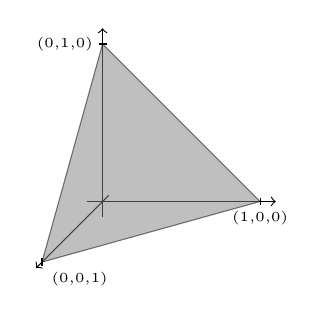
\begin{tikzpicture}[scale=2]
            \draw[->] (-0.1,0,0) -- (1.1,0,0);
            \draw[->] (0,-0.1,0) -- (0,1.1,0);
            \draw[->] (0,0,-0.1) -- (0,0,1.1);
            \draw (1,-0.025,0) -- (1,0.025,0);
            \draw (-0.025,1,0) -- (0.025,1,0);
            \draw (0,-0.025,1) -- (0,0.025,1);
    
            \node[anchor=north] at (1,0,0) {$\scriptscriptstyle(1,0,0)$};
            \node[anchor=east] at (0,1,0) {$\scriptscriptstyle(0,1,0)$};
            \node[anchor=north west] at (0,0,1) {$\scriptscriptstyle(0,0,1)$};
            \filldraw[fill=gray, opacity=0.5, draw=black] (1,0,0) -- (0,1,0) -- (0,0,1) -- (1,0,0);
        \end{tikzpicture}
        }
    \end{minipage}
    \scalebox{2}{
    \begin{minipage}[c]{0.01\textwidth}
            $\rightarrow$
    \end{minipage}
    }
    \begin{minipage}[c]{0.2\textwidth}
    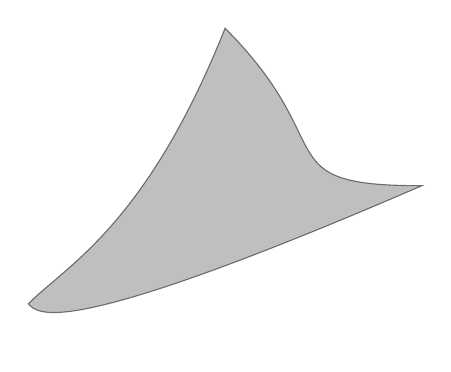
\begin{tikzpicture}[scale=0.5]
        \filldraw[fill=gray, draw=black, opacity=0.5] (0,0)  .. controls (0.25,-0.25) and (0.75,-1) .. (10,3)
            .. controls (6,3) and (8,4) .. (5,7)
            .. controls (3,2) and (1,1) .. (0,0) --cycle;
    \end{tikzpicture}
    \end{minipage}
    \caption{The standard 2-simplex and a $2$-simplex in the 2D plane i.e. 
    taking $X = \real^2$.}
    \label{fig:2simplex}
\end{figure}
See Fig.\,\ref{fig:1simplex} and Fig.\,\ref{fig:2simplex} for the 
standard 1- and 2-simplex and a possible singular simplex in the plane respectively.
As the term 'singular' implies these simplices can be degenerated. For example, $\sigma_k$ could 
just be constant, so the object in the topological space corresponding to the 
$k$-simplex is just a point.

We can now introduce an algebraic structure by looking at finite formal sums of the form 
\begin{align*}
    \sum_{\text{$\sigma$ $k$-simplex }} n_\sigma \sigma.
\end{align*}
These formal sums form an abelian group which we refer to as the 
\textit{singular $k$-chain group} $C_k(X)$. 
The next step is to introduce an important homomorphism between these groups called the \textit{boundary}.
\begin{definition}
    Let $\mathbf{v}_0, ... , \mathbf{v}_k \in \real^n$. 
    We define \textit{affine singular $k$-simplex} as a special singular $k$-simplex denoted by
    \begin{align*}
        [\mathbf{v}_0,...,\mathbf{v}_k]: \Delta_k \rightarrow \real^n, \, 
        \sum\limits_{i = 0}^k \lambda_i e_i \mapsto \sum\limits_{i = 0}^k \lambda_i \mathbf{v}_i.
    \end{align*}
\end{definition}
As in the general case, the image can be a degenerated simplex in $\real^n$ since the 
$\mathbf{v}_i$ are not assumed to be affine independent. 

We call the affine singular simplex 
\begin{align}
    [e_0,...,\hat{e}_i,...,e_k]: \Delta_{k-1} \rightarrow \Delta_k \label{eq:face_map}
\end{align}
the \textit{$i$-th face map} which we denote by $F^k_i$ and sometimes we will not write the superindex $k$. 
The $\hat{ }$ means this vertex is left out. Here we tacitly used the 
natural inclusion $\real^{k+1} \subseteq \real^\infty$ so we have 
$\Delta_k \subseteq \real^{k+1}$. But this is just a way of representation.
With the face map we can now define the boundary homomorphim.
\begin{definition}[Boundary]
    For a singular $k$-simplex $\sigma: \Delta_k \rightarrow X$ we define its $i$-th face 
    $\sigma^{(i)} \vcentcolon= \sigma \circ F_i^k$ which is a $(k-1)$-simplex. 
    We then define the \textit{boundary} of $\sigma$ as 
    $\partial_k \sigma \vcentcolon= \sum_{i=0}^k (-1)^i \sigma^{(i)}$. We extend this 
    to a homomorphism between the chain groups
    \begin{align*}
        \partial_k: C_k(X) \rightarrow C_{k-1}(X), 
        \sum_\sigma n_\sigma \sigma \mapsto \sum_\sigma n_\sigma \partial_k \sigma.
    \end{align*}
    In the case of $k=0$, we set $\partial_0 = 0$.
\end{definition}


\begin{figure}\centering
    \scalebox{2}{
        \begin{tikzpicture}
            \path [draw=black,postaction={on each segment={mid arrow=black}}]
                (-1,0) -- (1,0) -- (0,1.73205) -- (-1,0) --cycle;
        \end{tikzpicture}
    }
    \caption{A simplex with boundary. The boundary is the $1$-chain going around 
    the simplex in the given direction.}
    \label{fig:simplex_with_boundary}
\end{figure}


We will frequently leave out the subscript and just write $\partial$ for the boundary 
if it is clear from the context.
A straightforward computation (cf. \cite[Lemma 1.6]{topology_and_geometry}) shows the 
important property 
\begin{align*}
    \partial_k \circ \partial_{k+1} = 0
\end{align*}
which implies that $\Ima \partial_k\subseteq \ker \partial_{k-1}$ is 
a subgroup. We call a chain $c \in C_k(X)$ \textit{$k$-cycle} or \textit{closed} if $\partial_k c = 0$ and 
we call it \textit{$k$-boundary} or \textit{exact} if $c \in \Ima \partial_{k+1}$. 
Denote the group of $k$-cycles as $Z_k(X)$ and the $k$-boundaries as $B_k(X)$.
Since we are in the abelian setting this motivates us to define 
the resulting factor groups.
\begin{definition}[Homology groups]
    We define the \textit{$k$-th homology group} of the topological space $X$ as the factor group
    \begin{align*}
        H_k(X) \vcentcolon= \faktor{Z_k(X)}{B_k(X)}.
    \end{align*} 
\end{definition}
We denote the elements of the homology groups i.e. the equivalence classes of a 
$k$-cycle $c$ as $[c] \in H_k(X)$.

\begin{figure}
    \centering
    \begin{minipage}[c]{0.4\textwidth}
      \scalebox{2}{
        \begin{tikzpicture}
        \path [draw=black,postaction={on each segment={mid arrow=black}}]
            (0,1) arc [start angle=90, end angle=180, radius=1] 
            arc [start angle=180, end angle=270, radius=1]
            arc [start angle=270, end angle=360, radius=1]
            arc [start angle=0, end angle=90, radius=1];
        \draw [red,domain=125:415,->] plot ({0.4+0.1*cos(\x)}, {0.4+0.1*sin(\x)});
        \draw [red,domain=125:415,->] plot ({-0.4+0.1*cos(\x)}, {-0.4+0.1*sin(\x)});
        \draw [red,domain=125:415,->] plot ({-0.4+0.1*cos(\x)}, {0.4+0.1*sin(\x)});
        \draw [red,domain=125:415,->] plot ({0.4+0.1*cos(\x)}, {-0.4+0.1*sin(\x)});
        \draw (-1,0) -- (1,0);
        \draw (0,-1) -- (0,1);
        \end{tikzpicture}
      }
    \end{minipage}
    \begin{minipage}[c]{0.4\textwidth}
    \scalebox{2}{
      \begin{tikzpicture}
          \path [draw=black,postaction={on each segment={mid arrow=black}}]
              (0,1) arc [start angle=90, end angle=180, radius=1] 
              arc [start angle=180, end angle=270, radius=1]
              arc [start angle=270, end angle=360, radius=1]
              arc [start angle=0, end angle=90, radius=1];
          \filldraw[gray] (0,0) circle [radius=0.3];
      \end{tikzpicture}
    }
    \end{minipage}
    \caption{The $1$-chain around the circle on the left is exact since it is the boundary of the 
        $2$-chain formed by the sum of the four segments in the middle. The red circular arrows show the orientation. 
        The gray circle on the right 
        represents a whole in the domain and then the same $1$-chain around it is still closed, 
        but not exact anymore.}
\end{figure}
    

If the $k$-th homology group is finitely generated then we 
call the rank i.e. the number of generators the \textit{$k$-th Betti number}. 
These Betti numbers are fundamental properties of the topological space. 
For example, the zeroth Betti number corresponds to the number of 
path-components of the space. In 3 dimensions, the first Betti number of 
a compact domain
corresponds to the number of "holes", the second Betti number to the
number of enclosed "voids" in the domain \cite[p.14]{arnold}. E.g. a filled torus 
has the zeroth Betti number one, the first Betti number also equal to one
and the second equal to zero which can be proven using the Meyer-Vietoris sequence
(see \cite[Sec.\,IV.18]{topology_and_geometry}). We will not go into this in further detail
since we do not want to dwelve too deeply into algebraic topology.

This construction can be put in an abstract algebraic framework in the following 
way. We call a collection of abelian groups $C_i$, $i\in \integers$, a graded group.                                                   
Together with a collection of homomorphims $\partial_i: C_i \rightarrow C_{i-1}$ 
called \textit{differentials}
s.t. $\partial_{i-1} \circ \partial_i = 0$ this is called a \textit{chain complex} which 
we will denote by $C_*$. 

\begin{example}
    If we set $C_k(X) = {0}$ for $k < 0$ then the groups of $k$-chains with 
    the boundary operator form a chain complex . 
\end{example}

Completely analogous to above, we can define the homology groups 
of a abstract chain complex
\begin{align*}
    H_k(C_*) \vcentcolon= \faktor{\ker \partial_k}{\Ima \partial_{k+1}}.
\end{align*}

\begin{definition}[Chain map]
    Let $A_*$ and $B_*$ be chain complexes. With a slight abuse of notation
    let us denote the differentials of 
    both chain complexes just by $\partial$.
    Then a \textit{chain map} $f: A^* \rightarrow B^*$ is a collection 
    of homomorphisms $f_i: A_i \rightarrow B_i$ s.t. 
    $\partial \circ f_{i-1} = f_i \circ \partial$ i.e. the following diagram is commutative
    \begin{equation*}
        \begin{tikzcd}
            ... \arrow[r, "\partial"] 
                & A_{i+1} \arrow[r, "\partial"] \arrow[d, "f_{i+1}"] & A_i \arrow[r, "\partial"] \arrow[d, "f_i"] 
                & ...\\
            ... \arrow[r, "\partial"] 
                & B_{i+1} \arrow[r, "\partial"] & B_i \arrow[r, "\partial"] 
                & ...
        \end{tikzcd}
    \end{equation*}
\end{definition}
We will leave out the 
indices most of the time if it is clear what we mean.
The crucial property of these chain maps is that they induce homomorphisms of
the homology groups denoted as
\begin{align*}
    [f_i]: H_i(A_*) \rightarrow H_i(B_*), \, [f_i]([a]) = [f_i(a)]
\end{align*}

\subsection{Cohomology groups}\label{sec:cohomology_groups}

Let us start with the abstract definition of a cochain complex.
Let $\{ C^i \}_{i\in \naturalnum}$ be a collection of abelian groups
and homomorphisms $\partial^i: C^i \rightarrow C^{i+1}$ with 
$\partial^{i+1} \circ \partial^i = 0$ called \textit{codifferentials}. 
Then we call this sequence a 
\textit{cochain complex}. The only difference to chain complexes
is that the index 
increases when applying the codifferential. Hence, they are 
basically the same from an algebraic point of view.
By convention, 
we use superindices for anything that is related to cochain complexes. 

We define \textit{cochain maps} completely analogous to chain maps 
i.e. cochain maps commute with the codifferential.

The main motivation for cochain complexes comes from the 
\textit{singular cochain complexes} that we will introduce next.
Let $G$ be any abelian group and $X$ be a topological space as before. 
Then we define the group 
of \textit{$k$-cochains} $C^k(X;G)$ by
\begin{align*}
    C^k(X;G) \vcentcolon= \text{Hom}(C_k(X),\,G)
\end{align*}
i.e. the group of all homomorphisms from $k$-chains $C_k(X)$ to $G$. 
Just as for chains we now introduce a homomorphism between the groups of cochains
which transforms this into a cochain complex.
\begin{definition}[Coboundary ]
    We define the operator $\partial^k: C^k(X;G) \rightarrow C^{k+1}(X;G)$ via
    \begin{align*}
        (\partial^k f) (c) \vcentcolon= f(\partial_{k+1} c).
    \end{align*}
    for a $(k+1)$-chain $c$.
    We call a cochain $f \in C^k(X;G)$ \textit{closed} if $\partial^k f = 0$ 
    and we call $f$
    \textit{exact} if there is a $g \in C^{k-1}(X;G)$ s.t. $f = \partial^{k-1} g$.
    As for the boundary map we will frequently leave away the superscript if
    the context is clear.
\end{definition}
Notice that this naming is analogous to the naming for closed and exact forms. 
This is no coincidence as we will see in the Sec.\,\ref{sec:de_rhams_theorem}.

From the definition it is obvious that $\partial^{k+1} \circ \partial^{k} = 0$ 
and thus we have indeed a cochain complex which we call \textit{singular cochain 
complex}. If there is no confusion with the general notion of cochain complex
we will leave away the term 'singular'.
\begin{definition}[Singular cochain cohomology]
    Denote the closed $k$-cochains as $Z^k(X;G)$ and the 
    exact ones with $B^k(X;G)$. 
    We then define the \textit{cochain cohomology groups}
    $H^k(X;G)$ as
    \begin{align*}
        H^k(X;G) \vcentcolon= \faktor{Z^k(X;G)}{B^k(X;G)}.
    \end{align*}
\end{definition}
Note that in the case of $G = \real$ this becomes a vector space.
Now of course there is the question how the homology and cohomology groups 
are related to each other. This question is answered by the
\textit{universal coefficent theorem}. But before we can formulate it we have 
to introduce exact sequences.
\begin{definition}[Exact sequence] \label{def:exact_sequence}
    Let $(G_i)_{i\in \integers}$ be a sequence of groups and 
    $(f_i)_{i \in \integers}$ be a sequence of homomorphisms
    $f_i: G_i \rightarrow G_{i+1}$. Then this sequence of homomorphisms is
    called \textit{exact} if $\text{im}\,f_{i-1} = \text{ker}\,f_i$.
\end{definition}

The universal coefficent theorem in the case of homology states
that the sequence 
\begin{align}
    0 \rightarrow \text{Ext}(H_{k-1}(K),G) \rightarrow 
    H^k(K;G) \xrightarrow{\beta} \text{Hom}(H_k(K),G) 
    \rightarrow 0 \label{eq:univeral_coefficient_theorem}
\end{align}
is exact. 
$\beta$ is defined via 
\begin{align}
    \beta([F])([c]) \vcentcolon= F(c).
    \label{eq:isomorphism_from_universal_coefficent_theorem}
\end{align}
The definition of Ext can be found in \cite{topology_and_geometry},
but it does not matter for our purpose because from now on we will assume
$G = \real$ and in this case
$\text{Ext}(H_{k-1}(X),\real) = 0$. This follows from the fact that 
$\real$ is a divisible and hence injective abelian group. The definition of
these terms and their connections used can also be found in 
\cite[Sec.\,V.6]{topology_and_geometry}. However, we will not dwelve into the 
algebraic background further. In the case of $G = \real$, 
we can conclude from the exactness of the 
above short sequence that $\text{ker}\,\beta = 0$ and 
$\text{im}\,\beta = \text{Hom}(H_k(X),\real)$. So $\beta$ is an isomorphism 
and provides us with the link between the singular chains and cochains.


\subsection{De Rham's theorem} \label{sec:de_rhams_theorem}

It turns out that the singular cochain cohomology is closely related to the cohomology 
of differential forms, the \textit{de Rham cohomology} which is introduced next. 

Let $M$ be a smooth $n$-dimensional manifold.
We will use the notation introduced in 
Sec.\,\ref{sec:differential_forms_subsection}. Then the smooth 
differential forms $C^\infty \Lambda^k M$ together 
with the exterior derivative give us a cochain complex due to the property $d \circ d = 0$. 
This cochain complex is called
\textit{de Rham complex} . 
Note that we have slightly more structure here
since the $C^\infty \Lambda^k M$ are vector spaces and the exterior
derivative a linear map i.e. a vector space homomorphism.
Let us denote the exterior derivative on 
the space of $k$-forms as $d^k$. Then recall the notation
\begin{align*}
    \mathfrak{B}^k(M) &\vcentcolon= \Ima d^{k-1}
    \\ \mathfrak{Z}^k(M) &\vcentcolon= \ker d^k
\end{align*}
which are the exact and closed forms respectively.
We define $d^k = 0$ for $k < 0$ and $k>n$.
We then define the \textit{de Rham cohomology group} 
\begin{align*}
    H_{dR}^k(M) \vcentcolon= \faktor{\mathfrak{Z}^k(M)}{\mathfrak{B}^k(M)}
\end{align*}
It turns out that the de Rham complex is closely related with the 
singular cochain complex which is the topic of this section.

Let us recall Stokes' theorem first which said 
that for a $k$-form $\omega \in C_c^\infty \Lambda^k M$ 
on a smooth $k$-dimensional oriented manifold $M$ we have 
\begin{align*}
    \int_M d\omega = \int_{\partial M} \omega.
\end{align*}

The following details are taken from Section V.5 and V.9 of 
\cite{topology_and_geometry}. We will only focus on the main ideas and avoid 
dwelving into the technical details. The interested reader can find more 
arguments in the given reference.

Let now $\sigma$ be a smooth $k$-simplex i.e. $\sigma: \Delta_k \rightarrow 
M$ is smooth. We will solely focus on smooth simplices from now on. Let 
$C_k^{\text{smooth}}(M)$ be the abelian group generated by smooth $k$-simplices and 
then $H^k_{\text{smooth}}(M;\real)$ be the cochain groups constructed analogous to the 
standard case. Then in fact, 
$H^k_{\text{smooth}}(M;\real)$ and $H^k(M;\real)$ are isomorphic. This 
is the reason why it is sufficient for this section to deal with smooth simplices 
only and we will, by abuse of notation, refer to them as $C_k(M)$
and the homology groups as $H_k(M)$ etc.

We now define the integral over a $k$-simplex as
\begin{align*}
    \int_\sigma \omega = \int_{\Delta_k} \sigma^* \omega
\end{align*}
and then the integral over a $k$-chain 
$c = \sum_\sigma n_\sigma \sigma$
\begin{align*}
    \int_c \omega \vcentcolon= \sum \limits_\sigma n_\sigma \int_\sigma \omega.
\end{align*}
This motivates us to introduce the homomorphism $I: C^\infty \Lambda^k (M) 
\rightarrow \text{Hom}(C_k;\real)$ defined by 
\begin{align*}
    I(\omega)(c) = \int_c \omega.
\end{align*}
\begin{remark}
    There are some technical details that we will not discuss in detail here,
    but that should be mentioned. First, $\Delta_k$ is not a manifold. 
    The $(k-2)$-skeleton are the boundaries of the faces i.e. the corners for $k=2$ and the 
    edges for $k=3$. If we remove the $(k-2)$-skeleton 
    then $\Delta_k$ is a manifold 
    with boundary. But since this is a null-set w.r.t. the full simplex and 
    the boundary as well, this does not matter for our arguments. 
    Second, because we are integrating over the $\Delta_k$ their orientation is 
    important and has to be chosen consistently. We will not present the details here. The 
    only important fact is that the simplices are oriented in a way s.t.
    \begin{align}
        \int_{[e_0,...,\widehat{e_i}, ..., e_k]} \nu = (-1)^i \int_{\Delta_{k-1}} F_i^* \nu 
        \label{eq:integral_boundary_face}
    \end{align}
    for any integrable $(k-1)$-form on the face $[e_0,...,\widehat{e_i}, ..., e_k]$
    where the $F_i$ are the face maps defined at (\ref{eq:face_map})
    (see Fig.\,\ref{fig:simplex_with_boundary} for an illustration).
    Please consult \cite[Sec. V.5]{arnold} for more 
    details.
\end{remark}

% Now, 
% we have to remember the definition of the boundary of a singular simplex 
% and the face map $F^k_i$ which serves as a chart 
% of the $k-1$ dimensional manifold $[e_0,...,\widehat{e_i}, ..., e_k]$. 
Now we get from Stokes' theorem for a $k$-simplex $\sigma$
\begin{align*}
    I(d\omega)(\sigma) &= \int_\sigma d\omega 
    = \int_{\Delta_k} \sigma^* d\omega 
    = \int_{\Delta_k} d\sigma^* \omega
    = \int_{\partial \Delta_k} \sigma^* \omega
    \\ &= \sum_{i=0}^k \int_{[e_0,...,\widehat{e_i}, ..., e_k]} \sigma^* \omega
    \stackrel{(\ref{eq:integral_boundary_face})}{=} \sum_{i=0}^{k} (-1)^i \int_{\Delta_{k-1}} F_i^*\sigma^* \omega
    \\ &= \sum_{i=0}^{k} (-1)^i \int_{\Delta_{k-1}} (\sigma\circ F_i)^* \omega
    = \sum_{i=0}^{k} (-1)^i \int_{\sigma\circ F_i} \omega
    \\ &= I(\omega)(\partial \sigma) = \partial \big(I(\omega)\big) (\sigma).
\end{align*}
So we obtain
\begin{align*}
    I(d\omega) = \partial \big(I(\omega)\big).
\end{align*}
This means that $I$ is a cochain map and thus 
induces a homomorphism on cohomology
\begin{align*}
    [I]:H^k_{dR}(M) \rightarrow H^k(M;\real).
\end{align*}

Using the notation and the definition of this map we can now formulate 
de Rham's theorem which will become very important later when proving
existence and uniqueness in Sec.\,\ref{sec:existence_and_uniqueness}.
\begin{theorem}[De Rham's theorem]\label{thm:de_rhams_theorem}
    Let $M$ be a smooth orientable manifold. Then $[I]: H^k_{dR}(M) \rightarrow H^k(M;\real)$ is an isomorphism.
\end{theorem}
This is quite a deep result that requires more tools than we introduced and is
difficult to prove so we will just state it here. Even though it is a very short 
statement it has deep implications. It implies that the de Rham cohomology
reflects fundamental topological properties of the manifold. It provides a bridge 
between the two fields of differential geometry and algebraic topology.

\section{Hilbert complexes}\label{sec:hilbert_complexes}
We will now move away from geometry and topology to functional analysis.
A crucial tool for the proof will be the \textit{Hodge decomposition} 
in 3D which relies on unbounded operators and Hilbert complexes. These 
will be introduced in this section. This is essentially a 
recollection of the parts of chapter 3 and 4 of Arnold's book \cite{arnold}
that we will need. 

We start by introducing the concept of unbounded operators on real Hilbert spaces and 
the adjoint of these. Then we will apply this theory to 
the differential operators $\grad$, $\curl$ and $\diver$ in 3D. In the 
second part, we will introduce Hilbert complexes which combine the idea 
of cochain complexes and unbounded operators on Hilbert spaces. This will lead to the 
Hodge decomposition which is an important tool that we will need in the proof of 
existence and uniqueness.

Throughout this section 
it will be assumed that the reader is familiar with functional analysis, 
especially Hilbert spaces, 
and basic knowledge about Sobolev spaces. We will focus on real spaces 
exclusively.

\subsection{Unbounded operators}\label{sec:unbounded_operators}

We will provide the basic definitions about unbounded operators and propositions 
about those. After defining unbounded operators we will talk about closed and 
densely defined operators mainly and the adjoint. 
Most of the proofs are very short and we will be able to do them in detail. 

\begin{definition}[Unbounded operators]
    Let $X$ and $Y$ be Hilbert spaces. Then we call a linear mapping 
    $T: D(T) \rightarrow Y$ with a subspace $D(T) \subseteq Y$ an 
    \textit{unbounded 
    operator} from $X$ to $Y$. We call $D(T)$ the \textit{domain} of $T$.
\end{definition}
We will talk about an unbounded operator $T:X \rightarrow Y$ 
which means that $T$ is not necessarily defined on all of $X$. 

Note that this definition generalizes the standard operator. In particular, 
it includes the case when $T$ is in fact bounded which can be 
slightly confusing, but we will stick to this common naming convention. 

The domain is a crucial property of unbounded operators. We will sometimes 
denote the unbounded operator as the tuple $(T,D(T))$.
If $D(T)$ is dense in $X$ we call $T$ \textit{densely defined}. 
We say that two unbounded operators $T$ and $S$ from $X$ to $Y$ are equal 
if $D(T) = D(S)$ and $Tx = Sx$ for all $x\in D(T)$.

An easy
example of an unbounded densely defined operator is the classical gradient with 
the domain $C_0^1(\Omega) \subseteq L^2 (\Omega)$ 
with $\Omega \subseteq \real^n$ open i.e. here we have $X=L^2(\Omega)$ and 
$Y=L^2(\Omega;\real^n)$.
In short, $\grad$ is an unbounded operator from $L^2(\Omega)$ to 
$L^2(\Omega;\real^n)$ with domain $C_0^1(\Omega)$.
We could then denote it as $(\grad, C_0^1(\Omega))$. This also shows that 
the choice of domain is not unique. We could have instead chosen e.g. the 
different unbounded operator $(\grad, C_0^\infty (\Omega))$. 
Another example is the weak gradient with domain $H^1(\Omega)$ i.e.
$(\grad, H^1(\Omega))$. All of these unbounded operators mentioned are densely defined.

As for bounded operators we define the kernel or null space of an unbounded
operator 
\begin{align*}
    \ker T = \{ x \in D(T) \mid Tx = 0\}
\end{align*}
and the image or range
\begin{align*}
    \Ima T = \{ Tx \mid x \in D(T)\}.
\end{align*}
The only difference to keep in mind is that the unbounded operators are not 
defined on the whole $X$ in general.

Recall that the graph of a function $f: X \rightarrow Y$ is defined 
as $\{ (x,f(x)) \in X \times Y \mid x \in X\}$. 
Analogously, the graph of an unbounded operator $T$ is 
\begin{align*}
    \Gamma(T) \vcentcolon= \{ (x,Tx) \mid x \in D(T) \}
\end{align*}
which is obviously a subspace of $X\times Y$.

We define the \textit{graph inner product} on $D(T)$ as 
\begin{align*}
    \langle x,z \rangle _{D(T)} 
    \vcentcolon= \langle x,z \rangle _X + \langle Tx, Tz \rangle _Y,
    \quad x,z \in D(T).
\end{align*}
It is easy to show that this is indeed an inner product. We will call its 
induced norm the \textit{graph norm}
\begin{align*}
    \lVert x \rVert _{D(T)} = \sqrt{ \lVert x \rVert^2 _X + \lVert Tx \rVert ^2 _Y}
    , \quad x\in D(T).
\end{align*}
Even though this defines a norm, $D(T)$ might not be a Hilbert space 
because it is in general not complete w.r.t. this norm. Consider for example 
the unbounded operator $\grad: L^2(\Omega) \rightarrow L^2(\Omega;\real^n)$ with 
domain $C_0^\infty(\Omega)$ and $\Omega \subseteq \real^n$ open.
The graph norm is then 
\begin{align*}
    \lVert \phi \rVert _{D(\grad)} 
    = \sqrt{ \lVert \phi \rVert^2 _{L^2(\Omega)} + \lVert \grad \phi \rVert^2 
        _{L^2(\Omega)}}
        , \quad \phi \in C_0^\infty(\Omega)
\end{align*}
which is just the standard $H^1$-norm.
But it is well-known that $C_0^\infty(\Omega)$ is in fact not closed 
w.r.t. this norm and thus not complete 
since the completion of it is the space $H^1_0(\Omega)$ i.e. 
the Sobolev space with zero trace on the boundary. 
Below in Prop.\,\ref{prop:closed_operator_graph_norm}, we will provide a
sufficient and necessary condition for the domain to be a Hilbert space 
when the graph norm is used. 

The well-known closed graph theorem for bounded operators says that 
a linear operator from $X$ to $Y$ defined on all of $X$ 
(in contrast to unbounded operators in general) is bounded i.i.f. 
its graph is closed in $X\times Y$ w.r.t. the norm 
$\lVert (x,y) \rVert _{X\times Y} 
= \sqrt{\lVert x \rVert^2 _{X} + \lVert y \rVert^2 _{Y}}$. 
This motivates the following definition.

\begin{definition}[Closed operator]
    We call an unbounded operator $T:X \rightarrow Y$ \textit{closed} if 
    its graph $\Gamma(T)$ is closed w.r.t. the norm 
    $\lVert \cdot \rVert _{X\times Y}$.
\end{definition}
That means if we have a closed operator $T$ and
take a sequence $(x_n)_{n\in \naturalnum} \subseteq D(T)$
s.t. $x_n \xrightarrow{X} x$ and $Tx_n \xrightarrow{Y} y$ for some 
$x \in X$ and $y \in Y$. Then $(x_n,Tx_n) \xrightarrow{X\times Y} (x,y)$ and 
since $T$ is closed
$(x,y) \in \Gamma(T)$ i.e. $x \in D(T)$ and $Tx = y$. This is just 
a rephrasing of the definition essentially so this characterizes closed
operators equivalently.

\begin{proposition}\label{prop:closed_operator_graph_norm}
    An unbounded operator $T$ is closed i.i.f. its domain $D(T)$, endowed with the 
    graph inner product, is a Hilbert space.
\end{proposition}
\begin{proof}
    As mentioned above, the graph inner product is in fact an inner product 
    on $D(T)$. So we have to show completeness.
    Assume that $T$ is closed and take a sequence $(x_n)_{n \in \naturalnum} 
    \subseteq D(T)$ that is Cauchy w.r.t. the graph norm. That implies 
    that $(x_n)$ must be Cauchy w.r.t. the $X$-norm and $(Tx_n)$ must be 
    Cauchy w.r.t. the $Y$-norm so both sequences are convergent. Because $X$ and $Y$ are Hilbert spaces 
    there exists $x \in X$ s.t. $x_n \rightarrow x$ and $y \in Y$ s.t. 
    $Tx_n \rightarrow y$. Because $T$ is closed we know 
    $x \in D(T)$ so $D(T)$ is complete.

    For the other direction, assume $D(T)$ is complete and take a sequence 
    $(x_n)_{n \in \naturalnum} \subseteq D(T)$ s.t. $x_n \rightarrow x \in X$ 
    and $Tx_n \rightarrow y$ for some $y \in Y$. Because both sequences are 
    convergent they are both Cauchy and thus $(x_n)$ is Cauchy w.r.t. the
    graph norm. Due to the completeness of $D(T)$ that implies that $x \in D(T)$
    and $x_n \xrightarrow{D(T)} x$ and 
    \begin{align*}
        \lVert x_n - x \rVert^2 _{D(T)} 
        = \lVert x_n - x \rVert^2 _X + \lVert Tx_n - Tx \rVert^2 _Y 
        \rightarrow 0
    \end{align*}
    so $T x_n \rightarrow T x$ and thus $Tx = y$ which proves that 
    $T$ is closed.
\end{proof}

As an example, take the unbounded operator $(\grad, H^1(\Omega))$
i.e. the weak gradient as an unbounded operator 
from $L^2(\Omega)$ to $L^2(\Omega;\real^n)$ with 
domain $D(\grad) = H^1(\Omega)$. Then we described above that the 
graph norm here is just the $H^1$-norm. It is well-known that 
$H^1(\Omega)$ is a Hilbert space. Therefore 
Prop.\,\ref{prop:closed_operator_graph_norm} tells us that 
$(\grad, H^1(\Omega))$ is a closed operator in contrast to 
$(\grad, C_0^\infty(\Omega))$ as described above.

The adjoint of bounded operators can be generalized to unbounded operators 
as well. Let us derive this step by step. 
Assume $T: X \rightarrow Y$ is a densely defined unbounded operator. 
Let us fix a $y \in Y$ and 
look at the linear functional $\ell:D(T) \rightarrow \real$ given by
\begin{align*}
    \ell(x) = \langle y, Tx \rangle_Y.
\end{align*}
This functional is not necessarily bounded w.r.t. the norm on $X$. But if it is i.e. if $\ell \in D(T)'$ 
then because $D(T)$ is dense in $X$ we can extend it to a
$\bar{\ell} \in X'$. Let $v \in X$ be its Riesz representative. That means we have
\begin{align*}
    \langle v, x \rangle_X = \langle \ell, x \rangle_{X'\times X} = \langle y, Tx \rangle_Y 
        \quad \forall x \in D(T).
\end{align*}
$\langle \ell, x \rangle_{X'\times X}$ is the usual duality pairing and we will 
frequenty just write $\langle l, x \rangle$.
Then we define $v = T^* y$ and 
recognize this as the defining property of the adjoint and define 
\begin{align*}
    D(T^*) \vcentcolon= \{ y \in Y \mid \exists c_y \in \real:
        \,\langle y, Tx \rangle_Y \leq c_y \lVert x \rVert _X \quad\forall x \in X\}.
\end{align*}
It is easy to check that this is a linear subspace of $Y$.

\begin{proposition}
    $T^*: Y \rightarrow X $ is a linear unbounded operator with domain $D(T^*)$.
\end{proposition}
\begin{proof}
    Note first that $T^*y$ is well-defined for $y \in D(T^*)$ since the 
    $T^*y$ is the Riesz representative of $x \mapsto \langle y, Tx \rangle_Y$ 
    and the Riesz representative is well-known to be unique.

    We only have to show that $T^*$ is linear. Take $y_1, y_2 \in D(T^*)$ 
    and $\lambda \in \real$. Then
    \begin{align*}
        \langle T^*(y_1 + \lambda y_2), x \rangle _X
        &= \langle y_1 + \lambda y_2, Tx \rangle _Y
        = \langle T^*y_1, x \rangle + \lambda \langle T^*y_2, x \rangle
        \\ &= \langle T^*y_1 + \lambda T^*y_2, x\rangle_X.
    \end{align*}
    for all $x \in D(T)$. Because $D(T)$ is dense in $X$ this implies 
    $T^*(y_1 + \lambda y_2) = T^*y_1 + \lambda T^*y_2$.
\end{proof}

We would like to proof whether $T^*$ is itself densely defined or closed. 
This can be done in an elegant way by investigating the graphs of $T$ and 
$T^*$. But $\Gamma(T)$ is a subspace of $X\times Y$ and 
$\Gamma(T^*)$ of $Y\times X$. To compare the two, we introduce a rotation operator. 
For any real vector spaces $V$ and $W$ we define the rotation operator 
\begin{align*}
    R_{V\times W}: V\times W \rightarrow W \times V, (v,w) \mapsto (-w,v).
\end{align*}
It is obvious that $R_{V\times W}$ is an isometry when $V$ and $W$ are normed spaces  
and we have $R_{W,V}R_{V,W}Z = Z$ for any subspace $Z\subseteq V\times W$.
By using this rotation operator, we can formulate the following lemma.
\begin{lemma}\label{lem:rotated_graph}
    Let $T$ be a densely defined unbounded operator from $X$ to $Y$. 
    Then we have 
    \begin{align*}
        & \Gamma(T)^\perp = R_{Y,X}\Gamma(T^*) \text{ and}
        \\ &\overline{\Gamma(T)} = \big(R_{Y,X}\Gamma(T^*)\big)^\perp.
    \end{align*}
\end{lemma}
\begin{proof}
    $(x,y) \in \Gamma(T)^\perp$ holds i.i.f. 
    \begin{align*}
        0 = \langle (x,y), (v,Tv) \rangle _{X\times Y}
        = \langle x, v \rangle _X + \langle y, Tv \rangle _Y
            \quad \forall v \in D(T).
    \end{align*}
    i.e. 
    \begin{align*}
        \langle -x, v \rangle _X = \langle y, Tv \rangle _Y,
            \quad \forall v \in D(T).
    \end{align*}
    This is just equivalent to saying that $-x = T^*y$ i.e.
    \begin{align*}
        (x,y) = (-T^*y,y) \in R_{Y,X}\Gamma(T^*)
    \end{align*}
    which proves the first equality.

    For the second equivalence recall the basic fact from Hilbert space theory
    that for any subspace of a Hilbert space $V$,
    $(V^\perp)^\perp = \overline{V}$. Hence, applying the orthogonal 
    complement to both sides of the first equality gives us the second one.
\end{proof}

\begin{corollary}\label{cor:adjoint_of_densely_defined}
    The adjoint $T^*$ of a densely defined operator $T$ is closed. 
\end{corollary}
\begin{proof}
    Recall another basic fact from Hilbert space theory that the 
    orthogonal complement of a space is always closed. 
    So we know from the first equality that $R_{Y,X}\Gamma(T^*)$ is closed.
    Since $R_{Y,X}$ is an isometry we conclude that $\Gamma(T^*)$ is closed and 
    thus $T^*$ a closed unbounded operator.
\end{proof}

\begin{proposition}\label{prop:adjoint_of_densely_defined_closed}
    Let $T$ be a densely defined and closed unbounded operator.
    Then $T^*$ is also densely defined and closed.
\end{proposition}
\begin{proof}
    We know from the previous corollary that $T^*$ is closed. 
    In order to prove density, once again recall a fact from Hilbert space
    theory that a subspace is dense i.i.f. its orthogonal complement 
    is zero. So take $y \in D(T^*)^\perp$ arbitrary. We now have to show that 
    $y=0$ to complete the proof.
    \begin{align*}
        0 = \langle y, w \rangle_Y 
        = \langle 0, -T^*w \rangle _X + \langle y, w \rangle _Y
        = \langle (0,y), (-T^*w,w) \rangle _{X\times Y} \quad \forall w \in D(T^*)
    \end{align*}
    which just means
    \begin{align*}
        (0,y) \in \big(R_{Y,X}\Gamma(T^*)\big)^\perp 
        \stackrel{\text{Lemma\,\ref{lem:rotated_graph}} }{=} \overline{\Gamma(T)}
        = \Gamma(T).
    \end{align*}
    In the last line we used the fact, that $T$ is closed. 
    Thus $y = T0 = 0$ which concludes the proof.
\end{proof}

\begin{proposition}\label{prop:T_starstar_equals_T}
    If $T$ is a closed and densely defined operator, 
    then $T^{**} = T$.
\end{proposition}
\begin{proof}
    This is another application of Lemma \ref{lem:rotated_graph}. 
    Because $T$ is closed, $\Gamma(T) = \big( R_{Y,X}\Gamma(T^*)\big)^\perp$. 
    From the previous proposition, we know that $T^*$ is a closed and 
    densely defined operator as well and so $\Gamma(T^*) = \big( R_{X,Y}\Gamma(T^{**})\big)^\perp$.
    $T^{**}$ is closed and hence its graph as well, so
    from the properties of the rotation we know that
    \begin{align*}
        \Gamma(T^{**}) 
        &= \overline{\Gamma(T^{**})} 
        = \Gamma(T^{**})^{\perp \perp}
        = \big( R_{Y,X} R_{X,Y}\Gamma(T^{**})   \big)^{\perp \perp}
        \\ &= \Big( R_{Y,X}\big(R_{X,Y}\Gamma(T^{**})\big)^{\perp} \Big)^\perp
        = \Big( R_{Y,X} \Gamma(T^*) \Big)^\perp
        = \Gamma(T)
    \end{align*}
    Thus $T$ and $T^{**}$ have the same graph, which means that they are equal.
\end{proof}

We will now take a closer look at the kernels and images of unbounded operators.
Let us first notice a very clear result. If $T$ is a closed unbounded operator 
then its kernel $\ker T$ is closed. This follows indeed from the definition. 
But this is not true for the image $\Ima T$. Let us take
$(y_n)_{n \in \naturalnum} \subseteq \Ima T$ with $y_n \rightarrow y$.
If we now take the sequence $(x_n)_{n \in \naturalnum} \subseteq D(T)$
s.t. $Tx_n = y_n$ we do not know if $(x_n)$ converges or 
whether the limit is in $D(T)$ if it does converge. 
A very simple example is the inclusion operator
$\iota: H^1(\Omega) \rightarrow L^2(\Omega)$. This is actually a bounded 
operator and hence closed since 
\begin{align*}
    \lVert \iota f \rVert _{L^2(\Omega)} 
    = \lVert f \rVert _{L^2(\Omega)} 
    \leq \lVert f \rVert _{H^1(\Omega)},
\end{align*}
but its range $H^1(\Omega)$ is not closed in $L^2(\Omega)$.

Let us summarize the following relationships between the images and kernels 
of closed densely defined operators and their adjoints.

\begin{proposition}\label{prop:kernel_image_adjoint}
    Let $T: X \rightarrow Y$ be a closed densely defined operator. Then
    \begin{alignat*}{3}
        &\text{\normalfont{(i)}} \quad&&(\Ima T)^\perp &&= \ker T^*
        \\ &\text{\normalfont{(ii)}} \quad&&(\ker T)^\perp &&= \overline{\Ima(T^*)}
        \\ &\text{\normalfont{(iii)}} \quad&&(\Ima T^*)^\perp &&= \ker T
        \\ &\text{\normalfont{(iv)}} \quad&&(\ker T^*)^\perp &&= \overline{\Ima(T)}
    \end{alignat*}
\end{proposition}
\begin{proof}
    We will once again rely on Lemma\,\ref{lem:rotated_graph} about the 
    rotated graph. We will start with (iii)
    \begin{align*}
        x \in \ker T \Leftrightarrow (x,0) \in \Gamma(T) 
        \stackrel{\text{$T$ closed}}{=} \overline{\Gamma(T)} 
        = \big( R_{Y,X}\Gamma(T^*) \big)^\perp .
    \end{align*}
    This is equivalent to saying that for any $y \in D(T^*)$ 
    we have 
    \begin{align*}
        0 = \langle (x,0), (-T^*y,y) \rangle_{X \times Y}
        = \langle x, -T^*y \rangle_X
    \end{align*}
    which just means $x \in (\Ima T^*)^\perp$ and we proved (iii).

    (ii) follows from that immediately by taking the orthogonal complement 
    on both sides.

    From Prop.\,\ref{prop:adjoint_of_densely_defined_closed}, 
    we know that $T^*$ is closed and densely defined because $T$
    is. So the completely analogous reasoning with the roles of $T$ and $T^*$
    exchanged gives us (i) and taking the orthogonal complement again 
    proves (iv).
\end{proof}

\subsection{Adjoints of differential operators in 3D}\label{sec:adjoints_differential_operators_3d}

Let us investigate the situation in 3D with the common differential 
operators $\curl$, $\grad$ and $\diver$ on a domain $\Omega \subseteq \real^3$. 
At first, we only assume  $\Omega$ to be open, but we will later 
introduce some assumptions on the boundary of it. 


We will follow \cite[Sec.\,3.4]{arnold} for the most part. However, all the results in Arnold's book 
are provided for bounded domains only which is insufficient for our situation since 
we want to cover the case where $\Omega$ is unbounded with compact boundary. Thus, 
we will generalize the proofs provided in the reference to this case which always involves 
applying some additional cut-off type argument.

Take the unbounded operator 
$\diver: L^2(\Omega;\real^3) \rightarrow L^2(\Omega)$ with the smooth compactly supported 
vector valued functions
$C_0^\infty(\Omega;\real^3)$ as domain i.e. $(\diver, C_0^\infty(\Omega;\real^3))$ which 
we will from now on denote as $(\diver, C_0^\infty)$. At first, we recognize that 
the operator $(\diver, C_0^\infty(\Omega;\real^3))$ is densely defined and thus the adjoint exists.
When we take the adjoint of it then we know for $v \in 
D((\diver, C_0^\infty)^*)$
\begin{align*}
    \int_\Omega \diver ^* v \cdot \mathbf{u} \, dx
    = \int_\Omega v \, \diver \mathbf{u} \, dx \quad \forall 
    \mathbf{u} \in C_0^\infty(\Omega;\real^3).
\end{align*}
As before, vector valued quantites are written in bold.
Now if we take $\mathbf{u} = (u_1,0,0)^\top$ then 
\begin{align}
    \int_\Omega (\diver ^* v)_1 \, u_1 \, dx
    = \int_\Omega v \, \partial_1 u_1 \, dx \quad 
        \forall u_1 \in C_0^\infty \label{eq:adjoint_gradient_c0inf_components}
\end{align}
so we recognize that $-(\diver ^* v)_1$ is the weak derivative w.r.t. the 
first coordinate i.e. $-\partial_1 v$ and analogous for the other coordinates 
so we recognize $\diver^* = -\grad$. We further see that the
domain s.t. (\ref{eq:adjoint_gradient_c0inf_components}) is fulfilled is $H^1(\Omega)$ 
by definition. That means we showed 
\begin{align}
    (\diver, C_0^\infty)^* = (-\grad, H^1). \label{eq:adjoint_gradient_c0inf} 
\end{align}

We know from Cor.\,\ref{cor:adjoint_of_densely_defined} 
that the adjoint $(-\grad, H^1)$ is closed and 
we can conclude from Prop.\,\ref{prop:closed_operator_graph_norm} 
that $H^1(\Omega)$ is in fact a Hilbert space 
when using the graph norm which is the $H^1$-norm here. This provides an alternative 
way to derive this basic result.

Assume from now on that our domain $\Omega$ is a Lipschitz domain 
with compact boundary $\partial \Omega$. Note that $\Omega \subseteq \real^3$ 
can be unbounded. In the case of an exterior domain, i.e. when $\Omega$ is 
the complement of a compact set with Lipschitz boundary, this condition is trivially fulfilled.

Let us denote with $C^k_b(\overline{\Omega})$ the space of $k$ times continuously
differentiable functions with bounded support in $\overline{\Omega}$. 
In contrast to $C^k_0(\Omega)$ these functions are not necessarily zero on the 
boundary.
For $u \in C_b^1(\Omega)$, $\mathbf{v} \in C_b^1(\Omega;\real^3)$ we 
have the integration-by-parts formula
\begin{align}
    \int_\Omega u \, \diver \mathbf{v} \, dx
    = - \int_\Omega \grad u \cdot \mathbf{v} \, dx
        + \int_{\partial \Omega} u|_{\partial \Omega} \mathbf{v}\cdot\mathbf{n} \, ds
        \label{eq:integration_by_parts_C1}
\end{align}
where $\mathbf{n}$ is the unit normal which exists almost everywhere on the boundary of a 
Lipschitz domain. This formula is usually stated only for 
bounded domains (see \cite[Cor.\,3.20]{monk}), but when $\partial \Omega$ is compact 
we can simply reduce the domain 
because the supports of $u$ and $\mathbf{v}$ are both bounded. This is done using 
a standard cut-off argument.
To be precise, let $B_R \subseteq \real^3$ be the open ball around the origin 
with radius $R$ large enought s.t. $\partial \Omega \subseteq B_R$ and 
$\supp u \subseteq B_R$, $\supp \mathbf{v} \subseteq B_R$.
Define the reduced domain $\Omega_R \vcentcolon= \Omega \cap B_R$. 
Then because $u$ and $\mathbf{v}$ are both zero on $\partial B_R$
\begin{align*}
    \int_\Omega u \, \diver \mathbf{v} \, dx
    &= \int_{\Omega_R} u \, \diver \mathbf{v} \, dx
    \\ &= - \int_{\Omega_R} \grad u \cdot \mathbf{v} \, dx
        + \int_{\partial \Omega} u|_{\partial \Omega} \mathbf{v}\cdot\mathbf{n} \, ds
        + \int_{\partial B_R} u|_{\partial B_R} \mathbf{v}|_{\partial B_R} \cdot\mathbf{n} \, ds
    \\ &= - \int_\Omega \grad u \cdot \mathbf{v} \, dx
        + \int_{\partial \Omega} u|_{\partial \Omega} \mathbf{v}\cdot\mathbf{n} \, ds
\end{align*}
as claimed. This formula motivates us to define the divergence in a
weak sense.

\begin{definition}[Weak divergence]
    Let $\Omega \subseteq \real^3$ be open. For $\mathbf{v} \in L^2(\Omega;\real^3)$ we  
    define the space
    \begin{align*}
        H(\diver;\Omega) \vcentcolon= \bigg\{ \mathbf{v} \in L^2(\Omega;\real^3) &\mid
            \exists \sigma \in L^2(\Omega)\, \forall \phi \in C_0^\infty(\Omega) :  
            \\ &\quad\int_\Omega \sigma \, \phi \, dx = -\int_\Omega \mathbf{v} \cdot \grad \phi \, dx \bigg\}
    \end{align*}
    Then we call the $\sigma$ in the definition the \textit{weak divergence} of $\mathbf{v}$
    denoted by $\diver \mathbf{v}$.
\end{definition}
Using basic arguments from Sobolev theory this defines $\diver \mathbf{v}$ 
uniquely almost everywhere. 


We will frequently leave out the reference to the domain in the space definition.
We can immediately recognize from the definition that 
\begin{align}
    (\diver, H(\diver)) = (-\grad, C_0^\infty)^*. \label{eq:adjoint_grad_c0inf}
\end{align}

The next thing we want to talk about is the trace of $H(\diver)$. 
We will use the well-known properties of the trace in $H^1$. 
Let us recall 
quickly the definition of fractional order Sobolev spaces (cf. \cite[Sec.\,3.2]{monk}). Let 
$U \subseteq \real^n$ be an open domain. Take $m \in \naturalnum$, 
$s \in [0, 1)$ and $1 < p < \infty$. For a multiindex $\boldsymbol{\alpha} = 
(\alpha_1, \alpha_2, ..., \alpha_n)$ we define $|\boldsymbol{\alpha}| = \sum_{i=1}^n \alpha_i$ 
and denote 
\begin{align}
    \partial_{\bm{\alpha}} \phi = 
    \partial_{\alpha_1} \partial_{\alpha_2} \dots \partial_{\alpha_n} \phi.
\end{align}
Then we define the fractional Sobolev norm
\begin{align}
    \lVert u \rVert _ {W^{m+s, p}} = \left\{ \lVert u \rVert ^p_{W^{m, p}} + 
        \sum_{|\bm{\alpha}|=m} \int_U \int_U 
        \frac{|\partial_{\bm{\alpha}} u(x) - \partial_{\bm{\alpha}} u(y)|^p}
        {|x - y|^{n+sp}} \, dx \,dy\right\}^{1/p}\label{eq:fractional_sobolev_norm}
\end{align}
and the corresponding space $W^{m+s, p}(U) = \{ u \in W^{m,p}(U) \mid \lVert u \rVert _{W^{m+s, p}} < \infty \}$ 
which is a Banach space \cite[p.42]{monk}. We denote 
$H^{m+s}(U) = W^{m+s, 2}(U)$ as in the integer case. We will need the 
fractional Sobolev space over the boundary of a Lipschitz domain $U$. We assume 
again that the boundary is compact.
We define fractional order Sobolev spaces by taking the integrals of (\ref{eq:fractional_sobolev_norm}) 
over the boundary instead i.e. for $m = 0$
\begin{align*}
    \lVert u \rVert _{W^{s, p}(\partial \Omega)} = \left\{ \int_{\partial\Omega} |u|^p \, ds + 
        \int_{\partial\Omega} \int_{\partial\Omega}
        \frac{|u(x) - u(y)|^p}
        {|x - y|^{n-1+sp}} \, ds(x) ds(y)\right\}^{1/p}.
\end{align*}
Then it 
is a well-known result that $H^1(\Omega)$ has the trace operator 
$\tr: H^1(\Omega) \rightarrow H^{1/2}(\partial \Omega)$ which is surjective \cite[p.28]{arnold}.
We are trying to find something analogous for $H(\diver)$.

\begin{remark}
    The $H^1$ trace operator is usually defined only for bounded Lipschitz domains 
    (see \cite[Thm.\,3.9]{monk}), but it can be extended easily to unbounded Lipschitz domains with 
    compact boundary considering only values in some bounded subdomain. 
    To make this precise take an open ball centered at the origin $B_r$
    s.t. $\partial \Omega \subseteq B_r$. We denote $|\cdot |$ as the standard 
    Euclidian norm and
    define 
    \begin{align*}
        \chi_R(x) \vcentcolon= 
        \begin{cases}
            1 & |x| \leq R,
            \\ R + 1 - |x| & R < |x| < R+1,
            \\ 0 & \text{else}.
        \end{cases}        
    \end{align*}
    Let us denote 
    $\Omega_{R+1} \vcentcolon=  \Omega \cap B_{R+1}$
    To define the trace of a function $u \in H^1(\Omega)$ take the trace of
    $\chi_R u$ -- which has compact support in $\overline{B}_{R+1}$ -- 
    on $\Omega_R$ and restrict it to $\partial \Omega$ 
    i.e. $\tr u = \big( \tr_{\Omega_R} u\chi_R \big)|_{\partial \Omega}$.
    Then $tr: H^1(\Omega) \rightarrow H^{1/2}(\partial \Omega)$ is 
    surjective and with $C_R$ being the continuity constant of the trace on $\Omega_R$
    \begin{align*}
        \lVert \tr u \rVert _{H^{1/2}(\partial \Omega)}
        &= \lVert \tr_{\Omega_R} u\,\chi_R  \rVert _{H^{1/2}(\partial \Omega_R)}
        \leq C_R \lVert u\,\chi_R  \rVert _{H^1(\Omega_R)}
        = C_R \lVert u\,\chi_R  \rVert _{H^1(\Omega)}
        \\ &\leq \sqrt{3} C_R \lVert u  \rVert _{H^1(\Omega)}
    \end{align*}
    and thus the trace is bounded as well. The last inequality follows from 
    the expression of $\grad \chi_R$ and some standard estimates.
\end{remark}

We will start with the following abstract lemma. As is standard, for a bounded linear 
functional $\ell$ on a normed space $V$ we write $\langle \ell, v \rangle_{V'\times V} = \ell(v)$ 
or just $\langle \ell, v \rangle$.

\begin{lemma}\label{lem:dual_map_of_surjective_operator}
    Let $X, Y$ be Banach spaces and let $\gamma: X \rightarrow Y$ be a 
    linear bounded surjection with kernel $Z$. Then the dual map is defined as
    \begin{align*}
        \gamma': Y' \rightarrow X', \ell \mapsto \ell \circ \gamma
    \end{align*}
    or in product notation
    \begin{align*}
        \langle \gamma' \, \ell, x \rangle_{X' \times X} = \langle \ell, \gamma\,x \rangle_{Y'\times Y}.
    \end{align*}
    This dual map is then a bounded injection with image 
    being the annihilator of $Z$ which is defined as 
    $\{ f \in X' \mid f|_Z \equiv 0 \}$. In other words, if we have $f \in X'$
    with $\langle f, z \rangle = 0$ for all $z \in Z$ then there exists a unique 
    $g_f \in Y'$ s.t. $\langle f, x \rangle_{X' \times X} = \langle g_f, \gamma \, x \rangle_{Y'\times Y}$.
\end{lemma}
\begin{proof}
    Since $\gamma$ is bounded it is obviously a closed and densely defined 
    unbounded operator. Then we know from \cite[Thm.\,2.20]{brezis} that 
    $\gamma'$ is injective. Thm.\,2.19 in the same reference 
    then gives us that $\Ima \gamma'$ is the annihilator of $Z$. 
    The dual map is actually the adjoint in the generalized sense on Banach spaces 
    which is how the adjoint is defined in this reference. Then the 
    annihilator corresponds in that notation to "$Z^\perp$", but we will not use 
    this notation because we only introduced the adjoint for Hilbert spaces.
\end{proof}

We now want to apply this lemma to the trace. 
We follow the standard notation and write $H^{-1/2}$ for the dual space of 
$H^{1/2}$
\begin{proposition}\label{prop:existence_gl_in_H12}
    Let $\ell \in H^1(\Omega)'$ s.t. $\langle \ell, \sigma \rangle = 0$
    for all $\sigma \in H^1_0(\Omega)$. Then there exists a unique
    $g_\ell \in H^{-1/2}(\partial \Omega)$ s.t.
    \begin{align}
        \langle \ell, u \rangle_{H^1(\Omega)' \times H^1(\Omega)} 
        = \langle g_\ell, \tr u \rangle_{H^{1/2}(\partial \Omega)' \times H^{1/2}(\partial \Omega)}, 
            \quad \forall u \in H^1(\Omega). \label{eq:functional_as_trace_inner_product}
    \end{align}
    Also, there exist positive constants $C_1$ and $C_2$ s.t.
    
    \begin{align*}
        C_1 \lVert g_\ell \rVert _{H^{-1/2}(\partial \Omega)} \leq  \lVert \ell \rVert _{H^1(\Omega)'}
        \leq C_2 \lVert g_\ell \rVert _{H^{-1/2}(\partial \Omega)}.            
    \end{align*}
\end{proposition}
\begin{proof}
    Let us check the conditions of the lemma. We have the trace operator 
    $\tr: H^1(\Omega) \rightarrow H^{1/2}(\partial \Omega)$ as a 
    linear bounded surjection. So the conditions of 
    Lemma \ref{lem:dual_map_of_surjective_operator} are fulfilled 
    and (\ref{eq:functional_as_trace_inner_product}) follows.
    Using the fact that the $H^1$ trace is bounded we can estimate 
    \begin{align*}
        |\langle \ell, u \rangle| = |\langle g_\ell, \tr u \rangle|
        \leq C_2 \lVert g_\ell \rVert _{H^{-1/2}} \, \lVert u \rVert _{H^1} 
    \end{align*}
    for some constant $C_2>0$
    and thus $\lVert \ell \rVert _{H^1(\Omega)'} \leq C_2 \lVert g_\ell \rVert _{H^{-1/2}}$ . 
    For the inverse inequality,
    we take some $\mu \in H^{1/2}$. If we can find a $f \in H^1$ s.t. $\tr f = \mu$ and 
    \begin{align}
        \lVert f \rVert _{H^1} \leq 1/C_1 \lVert \mu \rVert _{H^{1/2}}\label{eq:existence_gl:bound_f}
    \end{align}
    holds then we can conclude
    \begin{align*}
        |\langle g_\ell, \mu \rangle| = |\langle \ell, f \rangle|
        \leq \lVert \ell \rVert _{H^1(\Omega)} \lVert f \rVert _{H^1}
        \leq \lVert \ell \rVert _{H^1(\Omega)} 1/C_1 \lVert \mu \rVert _{H^{1/2}}
    \end{align*}
    and thus $\lVert g_\ell \rVert _{H^{-1/2}} \leq 1/C_1 \lVert \ell \rVert _{H^1(\Omega)}$.

    We have to show that such an $f$ exists. This is true for bounded domains (cf. \cite[Thm.\,3.10]{ern_guermond}).
    To generalize it to unbounded domains with compact boundary, take an open ball $B_R$ centered at the 
    origin with radius $R$ large enough s.t. $\partial \Omega \subseteq B_R$ . 
    Then define 
    $\Omega_R = \Omega \cap B_R$.
    Take $f_R$ as a function s.t. $\tr f_R = \mu$ on $\partial \Omega$,  
    $\tr f_R = 0$ on $\partial B_R$ and 
    $\lVert f_R \rVert _{H^1(\Omega_R)} \leq C_R \lVert \tr f_R \rVert _{H^{1/2}(\Omega_R)}$
    for some $C_R > 0$ independent of $\mu$. 
    Because $\tr f_R = 0$ on $\partial B_R$ 
    we have $\lVert \tr f_R \rVert _{H^{1/2}(\partial \Omega_R)} 
    = \lVert \tr f_R \rVert _{H^{1/2}(\partial \Omega)}$
    and we can define $\bar{f}_R \in H^1(\Omega)$ by 
    extending $f$ by zero outside of $B_R$ so that 
    $\lVert \bar{f}_R \rVert _{H^1(\Omega)} = \lVert f_R \rVert _{H^1(\Omega_R)}$.
    To summarize,
    \begin{align*}
        \lVert \bar{f}_R \rVert _{H^1(\Omega)} = \lVert f_R \rVert _{H^1(\Omega_R)} 
        \leq C_R \lVert \tr f_R \rVert _{H^{1/2}(\Omega_R)}
        = C_R \lVert \tr f_R \rVert _{H^{1/2}(\partial \Omega)}
        = C_R \lVert \mu \rVert _{H^{1/2}(\partial \Omega)}
    \end{align*}
    so (\ref{eq:existence_gl:bound_f}) holds with $f = \bar{f}_R$ which completes the proof.
\end{proof}

We can now define a trace operator for $H(\diver)$.
\begin{theorem}[Trace of $H(\diver)$]\label{thm:trace_of_hdiv}
    The operator $\mathbf{v} \mapsto \langle \mathbf{v}|_{\partial \Omega} \cdot \mathbf{n}, \cdot
    \rangle_{L^2(\partial \Omega)} \in H^{-1/2}(\partial\Omega)$
    on $C^1_b(\overline{\Omega})$ can be extended to an operator 
    $\gamma_n: H(\diver;\Omega) \rightarrow H^{-1/2}$ s.t.
    \begin{align*}
        \int_\Omega \diver \mathbf{v} \,u \, dx 
        = -\int_\Omega \mathbf{v} \cdot \grad u \, dx + \langle \gamma_n \mathbf{v}, \tr u \rangle
    \end{align*}
    Also, analogous to the standard trace theorem, we have
    \begin{align*}
        \lVert \gamma_n \mathbf{v} \rVert _{H^{-1/2}(\Omega)} 
        \leq   \sqrt{2}  \lVert \mathbf{v}\rVert _{H(\diver; \Omega)}.
    \end{align*}
\end{theorem}
\begin{proof}
    % Now let us come back to the integration by parts formula. Let us take 
    % $u \in H^1(\Omega)$ and due to density find a sequence $(u^k)_{k \in \naturalnum} \subseteq C_b^\infty(\Omega)$ 
    % s.t. $u^k \xrightarrow{H^1} u$.
    % Then taking the limit on both sides of the integration by parts formula 
    % (\ref{eq:integration_by_parts_C1}) using the fact that 
    % that the trace operator is continuous and we see that 
    % integration by parts formula stays valid if $u \in H^1(\Omega)$. 
    Let us define 
    the linear functional $\ell_\mathbf{v} \in H^1(\Omega)'$ for a fixed $\mathbf{v} \in H(\diver)$
    as
    \begin{align*}
        \langle \ell_\mathbf{v}, u \rangle \vcentcolon= \int_\Omega u \, \diver \mathbf{v} \, dx 
         + \int_\Omega \grad u \cdot \mathbf{v} \, dx.
    \end{align*}
    Using Cauchy-Schwarz we get
    \begin{align*}
        \langle \ell_\mathbf{v}, u \rangle 
        \leq \sqrt{2} \lVert \mathbf{v} \rVert _{H(\diver)} \lVert u \rVert _{H^1} 
    \end{align*}
    and so $\ell_\mathbf{v}$ is indeed a linear bounded functional on $H^1$.
    
    Take $u \in H^1_0(\Omega)$. 
    Let $(u^k)_{k\in \naturalnum} \subseteq C^\infty_0$ s.t. 
    $u^k \xrightarrow{H^1} u$ which is possible due to density. 
    $\langle \ell_\mathbf{v}, u^k \rangle  = 0$  which follows directly from the  
    definition of the weak divergence and thus $\langle \ell_\mathbf{v}, u \rangle = 0$
    by continuity.

    We are in the situation of Prop.\,\ref{prop:existence_gl_in_H12} 
    and we find $\gamma_n \mathbf{v} \in H^{-1/2}(\partial \Omega)$ 
    s.t. 
    \begin{align*}
        \int_\Omega u \, \diver \mathbf{v} \, dx 
        + \int_\Omega \grad u \cdot \mathbf{v} \, dx 
        = \langle \gamma_n \mathbf{v}, \tr u \, \rangle \quad \forall u \in H^1(\Omega).
    \end{align*}
    
    The linearity of $\gamma_n$ is trivial to see.
    For the boundedness, using Cauchy-Schwarz 
    \begin{align*}
        \langle \gamma_n \mathbf{v}, \tr u \rangle 
        = \int_\Omega u \, \diver \mathbf{v} \, dx 
            + \int_\Omega \grad u \cdot \mathbf{v} \, dx
        \leq \sqrt{2} \lVert \mathbf{v} \rVert _{H(\diver)} \lVert u \rVert _{H^1}
    \end{align*}
    and so $\lVert \gamma_n \mathbf{v} \rVert _{H^{-1/2}} \leq \sqrt{2}\lVert \mathbf{v} \rVert _{H(\diver)}$
    which proves that $\gamma_n$ is indeed a bounded linear operator.
    %  The integration
    % by parts formula is fulfilled by construction. 

    Let us now look at the case when $\mathbf{v} \in C_b^1(\overline{\Omega}; \real^3)$.
    We know the integration-by-parts formula holds for all $u \in H^1$ as 
    explained above. We have
    \begin{align*}
        \langle \gamma_n \mathbf{v}, \tr u \rangle = 
        \int_\Omega u \, \diver \mathbf{v} \, dx 
            + \int_\Omega \grad u \cdot \mathbf{v} \, dx
        = \int_{\partial \Omega} \mathbf{v}\cdot \mathbf{n} \, \tr u \, ds.
    \end{align*}
    Due to the surjectivity of the trace of $H^1$ we get 
    \begin{align*}
        \langle \gamma_n \mathbf{v}, \cdot \rangle = \langle \mathbf{v} \cdot n, \cdot \rangle_{L^2(\partial\Omega)}.
    \end{align*}
    So in this sense the operator $\mathbf{v} \mapsto \langle \mathbf{v} \cdot n, \cdot \rangle_{L^2(\partial\Omega)} 
    \in H^{-1/2}$ extends to the bounded operator $\gamma_n: H(\diver) \rightarrow H^{-1/2}$.
\end{proof}
This theorem motivates us to recognize the normal trace as the natural trace 
on $H(\diver)$. Now we can define 
\begin{align*}
    H_0(\diver;\Omega) \vcentcolon= \{ \mathbf{v} \in H(\diver) \mid \gamma_n \mathbf{v}=0 \}.
\end{align*}

% \begin{proposition}
%     Under the given assumptions on the domain we have
%     \begin{align}
%         (\diver, H(\diver)) &= (\grad, H^1_0) \label{eq:adjoint_grad_h10}\\
%         (\grad, H^1) &= (\diver, H^1_0)\label{eq:adjoint_div_hdiv0}
%     \end{align}
% \end{proposition}
% \begin{proof}
%     We know from \ref{eq:adjoint_grad_c0inf} that 
%     \begin{align*}
%         (\diver, H(\diver)) = (\grad, C_0^ \infty).
%     \end{align*}
%     Take $\mathbf{v} \in H(\diver)$, $u \in H^1_0$ arbitrary and 
%     a sequence $(u^k)_{k\in \naturalnum} \subseteq C_0^\infty$ with 
%     $u^k \xrightarrow{H^1} u$. When we leave out the reference to the space of the 
%     inner product we mean the $L^2$ inner product. Then we know that 
%     \begin{align*}
%         \langle \diver \mathbf{v}, u^k \rangle = \langle \mathbf{v}, \grad u^k \rangle
%     \end{align*}
%     Taking the limit on both sides shows $\mathbf{v} \in D((\grad, H^1_0)^*)$ 
%     and $\grad^* \mathbf{v} = \diver \mathbf{v}$. 
%     Since $D((\grad,H^1_0)^*) \subseteq D((\grad,C_0^\infty)^*) = H(\diver)$ 
%     we get the other inclusion and the first equality follows.

    
%     At first, note that $H^1_0$ is densely defined so we can define the adjoint.
%     Since $(\diver, H(\diver)) = (\grad, C_0^\infty)^*$ and 
%     we know $D((\grad, H^1_0)^*) \subseteq H(\diver)$. 
%     If we now take 
%     $\mathbf{v} \in H(\diver)$ arbitrary, then we know from the 
%     extension of the integration-by-parts formula from Thm. \ref{thm:trace_of_hdiv}
%     \begin{align*}
%         \langle -\diver \mathbf{v}, u \rangle 
%         = \langle \mathbf{v}, \grad u \rangle + \langle \gamma_n \mathbf{v}, \tr u \rangle
%         = \langle \mathbf{v}, \grad u \rangle
%     \end{align*}
%     and thus $D((\grad, H^1_0)^*) \supseteq H(\diver)$. That shows \ref{}.

%     For the second claim the proof is completely analogous. We just use 
%     $\gamma_n \mathbf{v} = 0$ instead of $\tr u = 0$.
% \end{proof}

% By interchanging $\diver$ and $\grad$ in the above arguments we can conclude 
% \begin{align*}
%     (-\grad, C_0^\infty)^* = (\diver, H(\diver))
% \end{align*}
% where $H(\diver)$ is the domain of the adjoint which is equivalent to saying
% that for $\mathbf{u} \in H(\diver)$ there exists a $\tilde{v} \in L^2$ s.t.
% \begin{align*}
%     \int_\Omega \tilde{v} \phi \, dx = -\int_\Omega \mathbf{v} 
%         \cdot \grad \phi \, dx \quad \forall \phi \in C_0^\infty
% \end{align*}
% where we denote $\tilde{v} = \diver \mathbf{v}$ i.e. the weak divergence.

We know that $H^1$ contains all smooth functions 
$C_b^\infty(\overline{\Omega})$ which are dense in $L^2$. This follows easily 
from the fact that $C^\infty(\overline{\Omega})$ is dense in $H^1$ if $\Omega$ is bounded.
Analogously,
it can be shown that $C_b^\infty(\overline{\Omega};\real^3)$ is dense in $H(\diver)$ as well 
by using the fact that $C^\infty(\overline{\Omega};\real^3)$ is dense in $H(\diver)$ if $\Omega$
is bounded (\cite[Thm. 3.22]{monk}).
Hence, 
both of $(\grad,H^1)$ and $(\diver,H(\diver))$ are densely defined so 
their adjoints exist and we will compute them next. To do so, 
we need the following theorem.

\begin{theorem}[Surjectivity of $\gamma_n$]
    The operator $\gamma_n: H(\diver; \Omega) \rightarrow H^{-1/2}(\partial\Omega)$ 
    is surjective.
\end{theorem}
\begin{proof}
    Take $g \in H^{-1/2}(\Omega)$. As in previous proofs, take 
    the open ball $B_R$ centered at the origin with radius $R$ large enough 
    s.t. $\partial \Omega\subseteq B_R$ and define $\Omega_R = \Omega \cap B_R$.
    This is obviously a bounded Lipschitz domain with boundary 
    $\partial \Omega_R = \partial \Omega \, \dot{\cup} \,\partial B_R$.
    Then we take $u_R$ as the solution 
    of the problem 
    \begin{align*}
        -\Delta u_R + u_R &= 0 \text{ in $\Omega_R$}, \\
        u_R &= g \text{ on $\partial \Omega$ and} 
        \\ u_R &= 0 \text{ on $\partial B_R$.} 
    \end{align*}
    which reads in variational formulation
    \begin{align*}
        \int_{\Omega_R} \grad u_R \cdot \grad \phi \, dx + \int_{\Omega_R} u_R \, \phi \,dx 
        = \langle g, \tr \phi \rangle_{H^{-1/2}(\partial \Omega) \times H^{1/2}(\partial \Omega)} \quad \forall \phi \in H^1(\Omega_R).
    \end{align*}
    This problem has a unique solution since $\Omega_R$ is bounded (see \cite[Thm. 3.12]{monk}).
    Take $\mathbf{v} \vcentcolon= \grad u_R$. Then we see from the variational 
    formulation by choosing $\phi \in C_0^\infty(\Omega_R)$ that $u_R = \diver \mathbf{v}$.
    And then define $\bar{u}_R$ as the extension by zero outside of $B_R$ which is in $H^1$ 
    because $u_R = 0$ on $\partial B_R$ and take $\bar{\mathbf{v}} = \grad \bar{u}_R$. 
    Then $\diver \bar{\mathbf{v}} = \bar{u}_R$
    and for any $\phi \in H^1(\Omega)$
    \begin{align*}
        \langle \gamma_n \bar{\mathbf{v}}, \tr \phi \rangle 
        &= \int_\Omega \bar{\mathbf{v}} \cdot \grad \phi \, dx 
            + \int_\Omega \diver \bar{\mathbf{v}} \, \phi \, dx
        \\ &= \int_\Omega \grad \bar{u}_R \cdot \grad \phi \,dx
            + \int_\Omega \bar{u}_R \, \phi\, dx 
        \\ &= \int_{\Omega_R} \grad u_R \cdot \grad \phi\, dx
            + \int_{\Omega_R} u_R \, \phi \,dx 
        \\ &= \langle g, \tr \phi \rangle.
    \end{align*}
    Since the trace on $H^1$ is surjective we get $\gamma_n \mathbf{v} = g$.
\end{proof}
Now we can compute the adjoints of the operators $\grad$ and $\diver$ without boundary conditions.

\begin{theorem}\label{thm:adjoints_grad_div_without_bc}
    \begin{align}
        (-\diver, H_0(\diver)) &= (\grad, H^1)^* \\
        (-\grad, H_0^1) &= (\diver, H(\diver))^*
    \end{align}
\end{theorem}
\begin{proof}
    If we take $\mathbf{v} \in H_0(\diver)$ then we immediately get 
    from the integration by parts formula
    \begin{align*}
        \langle -\diver \mathbf{v}, u \rangle = \langle \mathbf{v}, \grad u \rangle \quad \forall u \in H^1
    \end{align*}
    and so $\mathbf{v} \in D((\grad, H^1)^*)$ and $\grad^* \mathbf{v} = -\diver \mathbf{v}$.
    The inner product is the $L^2$ inner product and we will from now denote the $L^2$ inner 
    product just by $\langle \cdot , \cdot \rangle$.
    Vice versa, take $\mathbf{v} \in D((\grad, H^1)^*)$. Then there exists 
    $\sigma \in L^2$ s.t.
    \begin{align*}
        \langle \mathbf{v}, \grad u\rangle = \langle \sigma, u \rangle
    \end{align*}
    for any $u \in H^1$. By choosing $u \in C_0^\infty$ we see 
    $\mathbf{v} \in H(\diver)$ and $\sigma = -\diver \mathbf{v}$. 
    Now taking again $u \in H^1$ arbitrary,
    \begin{align*}
        0 = \langle \mathbf{v}, \grad u \rangle + \langle \diver \mathbf{v}, u \rangle
        = \langle \gamma_n \mathbf{v}, \tr u \rangle
    \end{align*}
    and since $\tr$ is surjective we get $\gamma_n \mathbf{v} = 0$ i.e. 
    $\mathbf{v} \in H_0(\diver)$ and we have proven the first equality.

    Take $u \in D((\diver, H(\diver))^*)$. Then we already see
    \begin{align*}
        \int_\Omega \diver^*u \cdot \bm{\phi} \, dx
        = \int_\Omega u \diver \bm{\phi} \, dx \quad \forall \bm{\phi} \in C_0^\infty(\Omega;\real^3)
    \end{align*}
    and we can conclude due to (\ref{eq:adjoint_gradient_c0inf}) that $u \in H^1$ and
    $\diver^*u = -\grad u$. Then 
    \begin{align*}
        0 = \langle \grad u, \mathbf{v} \rangle
            + \langle u, \diver \mathbf{v} \rangle
        = \langle \gamma_n \mathbf{v}, \tr u \rangle.
    \end{align*}
    Now we use the surjectivity of $\gamma_n$ and see that 
    $\langle g, \tr u \rangle = 0$ for all $g \in H^{-1/2}(\partial \Omega)$ which 
    implies $\tr u = 0$ and thus $u \in H^1_0$. The other direction follows again 
    from the integration by parts formula immediately and we get 
    $D((\diver, H(\diver))^*) = H^1_0$ and the claim follows.
\end{proof}
This theorem provides us with an easy computation of the adjoints 
of the $\grad$ and $\diver$ with homogeneous boundary conditions.

\begin{corollary}
    \begin{align}
        (-\diver, H(\diver)) &= (\grad, H^1_0)^* \\
        (-\grad, H^1) &= (\diver, H_0(\diver))^*
    \end{align}
\end{corollary}
\begin{proof}
    $(\diver, H(\diver))$ is the adjoint of the densely defined operator 
    $(-\grad, C_0^\infty)$ and hence a closed operator. It is 
    obviously densely defined and thus we can use previous results,
    \begin{align*}
        (\diver, H(\diver)) 
        \stackrel{Prop.\,\ref{prop:T_starstar_equals_T}}{=}(\diver, H(\diver))^{**} 
        \stackrel{Thm.\,\ref{thm:adjoints_grad_div_without_bc}}{=}(-\grad, H^1_0)^*.
    \end{align*}
    The adjoint of $(\diver, H_0(\diver))$ is computed completely analogously.
\end{proof}

% That begs the question what in turn the adjoints of 
% $(\grad,H^1)$ and $(\diver, H(\diver))$ are. 
% In order to answer it, we take a look at the standard 
% integration-by-parts formula assuming $\Omega$ is a Lipschitz domain
% \begin{align}
%     \int_\Omega u \, \diver \mathbf{w} \, dx 
%         + \int_\Omega \grad u \cdot \mathbf{w} \, dx
%     = \int_{\partial \Omega} u \, \mathbf{w}\cdot n \, ds
%     \label{eq:integration_by_parts}
% \end{align}
% where $n$ is the outward unit normal of $\Omega$. If we want 
% $u \in D(\diver)$ then the boundary integral on the right hand side must 
% vanish which would be the case if $u$ is zero on the boundary. 

% We can now take two approaches. The first one follows \cite{picard} by 
% saying a $u\in H^1$ has \textit{zero boundary conditions} 
% i.i.f. the right hand side vanishes for any $\mathbf{w} \in H(\diver)$. 
% This has the advantage that this 
% definition makes sense on any domain $\Omega$ independent of the regularity of 
% the boundary. 

% The other approach followed by Arnold defines the trace operators. 
% For $H^1$ this is very basic and leads to the classic trace operator 
% $\tr : H^1(\Omega) \rightarrow H^{1/2}(\Omega)$ assuming $\Omega$ has a 
% Lipschitz boundary. Then we find 
% $(\diver, H(\diver))^* = H^1_0(\Omega)$ where $H^1_0(\Omega)$ is the 
% space of $H^1$-functions with zero trace. Then we obtain 
% \begin{align*}
%     (\diver, H(\diver))^* = (-\grad, H^1_0).
% \end{align*}

% Vice versa, we see that if $u$ is non-zero on the boundary then 
% $\mathbf{w}\cdot n$ has to vanish. We can give mean to this for functions 
% in $H(\diver)$ by defining a operator $\gamma_n: H(\div) \rightarrow H^{-1/2}$ 
% s.t. if $\mathbf{w}$ is differentiable then 
% $\gamma_n(\mathbf{w}) = \mathbf{w} \cdot n$. Then we would define 
% \begin{align*}
%     \mathring{H}(\div) = \{ \mathbf{w} \in H(\diver) \mid \gamma_n\, \mathbf{w} 
%         = 0 \}
% \end{align*}
% and we get
% \begin{align*}
%     (\grad, H^1)^* = (\diver, \mathring{H}(\diver)).
% \end{align*}


This completes the computation of the adjoints of $\grad$ and $\diver$. Because  
$(\diver, H(\diver))$ is a closed and densely defined operator 
by taking the graph inner product on $H(\diver)$
\begin{align*}
    \langle \mathbf{v}, \mathbf{w} \rangle _{H(\diver)}
    \vcentcolon= \langle \mathbf{v}, \mathbf{w} \rangle + \langle \diver \mathbf{v}, \diver \mathbf{w} \rangle
\end{align*}
and the induced norm,
we know from Prop. \ref{prop:closed_operator_graph_norm} that $H(\diver)$ becomes a Hilbert space.

\begin{remark}
    Notice that in the above arguments 
    we never used the fact that we are working in three dimensions. Thus, 
    all the arguments can be generalized to $n$ dimensions without problems.
\end{remark}

Now let us turn our attention to the remaining fundamental differential operator 
$\curl$. For 
$\mathbf{u}, \mathbf{v} \in C^1(\overline{\Omega};\real^3)$ we have the well-known integration-by-parts 
formula
\begin{align}
    \int_\Omega \mathbf{v} \cdot \curl \mathbf{u} \, dx 
    = \int_\Omega \curl \mathbf{v} \cdot \mathbf{u} \, dx 
        + \int_{\partial \Omega} \mathbf{v} \times \mathbf{n} \cdot \mathbf{u} \, ds 
        \label{eq:integration_by_parts_curl_C1} 
\end{align}
if $\Omega$ is bounded and Lipschitz. Just as before, this integration by parts formula can 
be extended to $\Omega$ unbounded when $\partial \Omega$ is compact. 
We define as before 
\begin{definition}
    Let $\Omega \subseteq \real^3$ be an open domain. 
    Then we define 
    \begin{align*}
        H(\curl;\Omega) \vcentcolon= \bigg\{ \mathbf{v} \in L^2(\Omega;\real^3)
        &\mid \exists \mathbf{w} \in L^2(\Omega; \real^3) 
        \,\forall \boldsymbol{\phi} \in C_0^\infty(\Omega;\real^3):
        \\ &\quad \int_\Omega \mathbf{w} \cdot \boldsymbol{\phi} \, dx 
        = \int_\Omega \mathbf{v} \cdot \curl \boldsymbol{\phi} \, dx \bigg\}
    \end{align*}
    and we denote $\mathbf{w} = \curl \mathbf{v}$.
\end{definition}
From the definition we can see
\begin{align*}
    (\curl, H(\curl)) = (\curl, C_0^\infty)^*.
\end{align*}
Following analogous arguments as above, we obtain the following 
\begin{theorem}\label{thm:trace_hcurl}
    Let $\Omega$ be a Lipschitz domain with compact boundary $\partial \Omega$.
    Then the operator $\mathbf{v} \mapsto 
    \langle \mathbf{v}|_{\partial \Omega} \times \mathbf{n}, \,\cdot\, \rangle_{L^2(\partial \Omega)}$ 
    defined on $C^1_b(\overline{\Omega};\real^3)$ extends to a bounded linear operator 
    $\gamma_\tau: H(\curl) \rightarrow H^{-1/2}(\partial \Omega; \real^3)$ 
    s.t. the integration-by-parts formula 
    \begin{align*}
        \int_\Omega \curl \mathbf{v} \cdot \mathbf{u} \, dx = 
            \int_\Omega \mathbf{v} \cdot \curl \mathbf{u} \, dx
            + \langle \gamma_\tau \mathbf{v}, \mathbf{u} \rangle
    \end{align*}
    for all $\mathbf{v} \in H(\curl), \mathbf{u} \in H^1(\Omega;\real^3)$
    is satisfied and there exists $C>0$ s.t.
    $\lVert \gamma_\tau \mathbf{v} \rVert _{H^{-1/2}(\partial \Omega; \real^3)} 
    \leq C \lVert \mathbf{v} \rVert _{H(\curl)}$. 
\end{theorem}
Analogous to before, we define 
\begin{align*}
    H_0(\curl) \vcentcolon= \{ \mathbf{v} \in H(\curl) \mid \gamma_\tau \mathbf{v} = 0\}.
\end{align*}
Using this definition we can compute the adjoint.
\begin{theorem}
    We have the adjoints
    \begin{align*}
        (\curl, H_0(\curl)) &= (\curl, H(\curl))^* \text{ and }
        \\ (\curl, H(\curl)) &= (\curl, H_0(\curl))^*.
    \end{align*}
\end{theorem}
\begin{proof}
    Take $\mathbf{v} \in D((\curl, H(\curl))^*)$. 
    \begin{align*}
        \int_\Omega \curl^*\mathbf{v} \cdot \boldsymbol{\phi} \, dx
        = \int_\Omega \mathbf{v} \cdot \curl \boldsymbol{\phi} \, dx
            \quad \forall \boldsymbol{\phi} \in C_0^\infty(\Omega;\real^3)
    \end{align*}
    and thus $\curl^* \mathbf{v} = \curl \mathbf{v}$ and we have 
    \begin{align}
        \langle \curl \mathbf{v}, \mathbf{w} \rangle
        = \langle \mathbf{v}, \curl \mathbf{w} \rangle \label{eq:adjoint_curl_equation}
    \end{align}
    for all $\mathbf{w} \in H(\curl)$. That means that for $\mathbf{w} \in H^1(\Omega;\real^3)$
    \begin{align*}
        \langle \gamma_\tau \mathbf{v}, \tr \mathbf{w} \rangle 
        =  \langle \curl \mathbf{v}, \mathbf{w} \rangle - \langle \mathbf{v}, \curl \mathbf{w} \rangle
        = 0
    \end{align*}
    and thus $\gamma_\tau \mathbf{v} = 0$ i.e. $\mathbf{v} \in H_0(\curl)$.

    Vice versa, take $\mathbf{v} \in H_0(\curl)$. Then we need to show that 
    (\ref{eq:adjoint_curl_equation}) is fulfilled and we would like to use the integration-by-parts formula 
    for that. However, this formula only holds for $\mathbf{w} \in H^1(\Omega;\real^3)$. 
    We need to use the fact that $C_b^\infty(\overline{\Omega};\real^3)$ is 
    dense in $H(\curl)$. Analogous to what we have done before, the argument follows easily from the fact that 
    for bounded domains $U$, $C^\infty(\overline{U};\real^3)$ is dense in $H(\curl;U)$. 
    The statement for bounded domains is proven in \cite[Lemma 3.27]{monk}. 
    The proof is quite technical 
    and we will not present it here. But using the density it is clear that 
    $H^1(\Omega;\real^3)$ is also dense in $H(\curl)$ since it contains all smooth functions 
    with bounded support. Take $\mathbf{w} \in H(\curl)$ arbitrary and 
    $(\mathbf{w}^k)_{k \in \naturalnum} \subseteq H^1(\Omega;\real^3)$
    s.t. $\mathbf{w}^k \xrightarrow{H(\curl)} \mathbf{w}$.
    Because $\gamma_\tau \mathbf{v} = 0$ we have 
    \begin{align*}
        \langle \curl \mathbf{v}, \mathbf{w}^k \rangle
        = \langle \mathbf{v}, \curl \mathbf{w}^k \rangle
    \end{align*}
    Now taking the limits on both sides and using the fact that $\mathbf{w}$ was 
    arbitrary we get $\mathbf{v} \in D((\curl, H(\curl))^*)$ and 
    we obtain the first equality. 

    The second equality follows from the fact that $(\curl, H(\curl))$ is 
    a closed and densely defined operator and thus 
    \begin{align*}
        (\curl, H(\curl))= (\curl, H(\curl))^{**} = (\curl, H_0(\curl))^*.
    \end{align*}
\end{proof}
With this, we computed the adjoints of the most important differential operators that 
will be needed in the following section. 

\subsection{Hilbert complexes}\label{sec:hilbert_complexes_subsection}

Now we will combine the idea of cochain complexes from Section 
\ref{sec:singular_homology} 
with unbounded operators. We will  
derive the Hodge decomposition with the theory of unbounded operators of 
Sec.\,\ref{sec:unbounded_operators} and apply it to the three dimensional case
using the results of Sec.\,\ref{sec:adjoints_differential_operators_3d} about the 
differential operators in 3D.

Recall that a cochain complex 
is in full generality a sequence of groups $(G^i)_{i\in \integers}$ 
and group homomorphims $f^i: G^i \rightarrow G^{i+1}$ s.t. 
$f^{i+1} \circ f^{i} = 0$.

\begin{definition}[Hilbert complex]
    A Hilbert complex is a sequence of real Hilbert spaces $(W^k)_{k\in \integers}$
    and a sequence of closed, densely defined 
    unbounded operators $d^k: W^k \rightarrow W^{k+1}$ with domain
    $V^k \subseteq W^k$ s.t. $d^{k+1} \circ d^k = 0$.
\end{definition}
\noindent We denote $\mathfrak{Z}^k  \vcentcolon= \ker d^k$ and $\mathfrak{B}^k 
\vcentcolon= \Ima d^{k-1}$. Then it follows from the definition that
$\mathfrak{B}^k \subseteq \mathfrak{Z}^k$. 

To be precise, a Hilbert complex is in fact not a cochain complex in the exact 
sense because the homomorphims $d^k$ are not defined on the whole space, but it is if we look at
the operators defined on their domains $V^k$ instead.

Because unbounded operators are bounded w.r.t. the graph norm,
the restriction of the operators to their domain,
$d^k: V^k \rightarrow V^{k+1}$, are bounded operators when we use the graph norm
on $V^k$. 
% Note that $\mathfrak{B}^{k+1} \subseteq \mathfrak{Z}^{k+1} 
% \subseteq V^{k+1}$
% so this is well-defined. 
Because we assume $d^k$ to be 
closed we know from Prop.\,\ref{prop:closed_operator_graph_norm}
that $V^k$ are Hilbert spaces w.r.t. the graph norm $\lVert \cdot \rVert _{V^k}$.
So we see that $d^k$ together with $V^k$ is also a Hilbert complex which 
we call \textit{domain complex}. In this Hilbert complex, all operators are 
bounded. Notice since the operators are defined on the whole Hilbert space 
$V^k$ this fits the definition of a cochain complex, because vector spaces 
with summation
are groups and the $d^k$ are linear mappings and hence group homomorphisms.

Now let us investigate the adjoints of the operators in a Hilbert complex.
Since we assume the operators to be closed and densely defined the adjoints 
exist and we denote with $d_k^*:W^k \rightarrow W^{k-1}$ the adjoint of $d^k$.
Due to Prop.\,\ref{prop:adjoint_of_densely_defined_closed} we know that the 
adjoints are also closed and densely defined. We denote 
$V_k^* \vcentcolon= D(d_k^*)$, $\mathfrak{Z}^*_k \vcentcolon= \ker d^*_k$ 
and $\mathfrak{B}^*_k \vcentcolon= \Ima d^*_k$. We will frequently leave out 
the indices from now on.

We can apply Prop.\,\ref{prop:kernel_image_adjoint} to this construction. 
Then we observe 
\begin{align*}
    \mathfrak{B}^\perp &= \mathfrak{Z}^*,
    \\ \mathfrak{Z}^\perp &= \overline{\mathfrak{B}^*},
    \\ \mathfrak{B^*}^\perp &= \mathfrak{Z} \text{ and}
    \\ \mathfrak{Z^*}^\perp &= \overline{\mathfrak{B}^*}.
\end{align*}
Now recall the basic fact from Hilbert space theory that 
in any Hilbert space if we have any two subspaces $V \subseteq W$ then taking the 
orthogonal complements reverses the inclusion i.e.
$V^\perp \supseteq W^\perp$. Then we get 
\begin{align}
    \mathfrak{B}^* \subseteq \overline{\mathfrak{B}^*} 
    = \mathfrak{Z}^\perp  \subseteq \mathfrak{B}^\perp 
    = \mathfrak{Z}^*. \label{eq:image_kernel_of_adjoint_in_hilbert_complex}
\end{align}
We call 
\begin{align*}
    \dots \xrightarrow{d^*_{k+2}} V^*_{k+1}  \xrightarrow{d^*_{k+1}} V^*_{k}
    \xrightarrow{d^*_{k}} V^*_{k-1} \xrightarrow{d^*_{k-1}} \dots
\end{align*}
the \textit{dual complex} of the Hilbert complex.

\begin{definition}
    We call a $v \in V^k \cap V^*_k$ \textit{harmonic form} if $d^k v = 0$ and 
    $d^*_k v = 0$. Denote the space of harmonic forms as 
    $\mathfrak{H}^k$.
\end{definition}
\noindent We can rewrite this as $\mathfrak{H}^k = \mathfrak{Z}^k 
\cap \mathfrak{Z}^*_k$. Using 
(\ref{eq:image_kernel_of_adjoint_in_hilbert_complex},
\begin{align*}
    \mathfrak{H}^k = \mathfrak{Z}^k \cap \mathfrak{B}^{k,\perp}
         = \mathfrak{B}_k^{*,\perp} \cap \mathfrak{Z}^*_k.
\end{align*}
Now we can formulate the most important 
result of this chapter. 

\begin{theorem}[Hodge decomposition]\label{thm:hodge_decomposition}
    Let $d^k: W^k \rightarrow W^{k+1}$ form a Hilbert complex. 
    Then we have
    \begin{align*}
        \mathfrak{Z}^k &= \overline{\mathfrak{B}^k} \stackrel{\perp}{\oplus}
            \mathfrak{H}^k \text{ and}
        \\ \mathfrak{Z}^*_k &= 
            \overline{\mathfrak{B}^*_k} \stackrel{\perp}{\oplus}
            \mathfrak{H}^k.
    \end{align*}
    We obtain the Hodge decomposition of the space $W^k$
    \begin{align*}
        W^k = \overline{\mathfrak{B}^k} \stackrel{\perp}{\oplus}
            \mathfrak{H}^k \stackrel{\perp}{\oplus} \overline{\mathfrak{B}^*_k}.
    \end{align*}
\end{theorem}
\begin{proof}
    Let us first prove $\mathfrak{Z}^k \subseteq 
    \overline{\mathfrak{B}^k} \stackrel{\perp}{\oplus} \mathfrak{H}^k$.
    Take $z \in \mathfrak{Z}^k$ arbitrary. 
    From basic Hilbert theory we know that 
    $W^k = \overline{\mathfrak{B}^k} \stackrel{\perp}{\oplus} 
    \mathfrak{B}^{k,\perp}$. So we find $z = z_1 + z_2$ with
    $z_1 \in \overline{\mathfrak{B}^k}$ and $z_2 \in 
    \mathfrak{B}^{k,\perp}$. 
    Because $\mathfrak{Z}^k$ is closed 
    $z_1 \in \overline{\mathfrak{B}^k} \subseteq \mathfrak{Z}^k$ 
    and thus $z_2 = z - z_1 \in \mathfrak{Z}^k$ as well i.e. $z_2 \in \mathfrak{Z}^k 
    \cap \mathfrak{B}^{k,\perp} = \mathfrak{H}^k$ and so 
    $z \in \overline{\mathfrak{B}^k} \stackrel{\perp}{\oplus}
    \mathfrak{H}^k$. The other inclusion is obvious since 
    $\mathfrak{H}^k = \mathfrak{B}^{k,\perp} \cap \mathfrak{Z}^k$.
    The proof for the second equality is completely analogous. 

    For the Hodge decomposition, since $\mathfrak{Z}^k$ is closed 
    \begin{align*}
        W^k = \mathfrak{Z}^k \stackrel{\perp}{\oplus} \mathfrak{Z}^{k,\perp}
        =  \overline{\mathfrak{B}^k} \stackrel{\perp}{\oplus}
            \mathfrak{H}^k \stackrel{\perp}{\oplus} \overline{\mathfrak{B}^*_k}.
    \end{align*}
\end{proof}
The Hodge decomposition is a very powerful tool whenever we deal with Hilbert
complexes. Another important result will be the Poincaré inequality 
in the case where $\mathfrak{B}^k$ is closed.

\begin{theorem}[Poincaré inequality] \label{thm:poincare_inequality}
    For any $k$, if $\mathfrak{B}^{k+1}$ is closed in $V$ then there exists a 
    $c_{P,k}>0$ s.t. 
    \begin{align*}
        \lVert z \rVert _V \leq c_{P,k} \lVert dz \rVert, \quad \forall z \in \mathfrak{Z}^{k,\perp_V}
    \end{align*}
    where $\perp_V$ denotes the orthogonal complement w.r.t. the $V$-inner product.
\end{theorem}
\begin{proof}
    This follows directly form the Banach inverse theorem. Because $\mathfrak{B}^{k+1}$ is closed
    it is itself a Hilbert space. If we restrict $d^k$ to $\mathfrak{Z}^{k,\perp_V}$ it 
    is injective and so $d^k|_{\mathfrak{Z}^{k,\perp_V}}:\mathfrak{Z}^{k,\perp_V} 
    \rightarrow \mathfrak{B}^{k+1}$ is a bounded isomorphism between 
    Hilbert spaces and we can apply the Banach inverse theorem to obtain the inverse 
    denoted by slight abuse of notation as $d^{-1}$ which is also bounded. So 
    for any $z \in \mathfrak{Z}^{k,\perp_V}$
    \begin{align*}
        \lVert z \rVert _V = \lVert d^{-1} dz \rVert _V  \leq c_{P,k} \lVert dz \rVert _V 
        = c_{P,k} \lVert dz \rVert.
    \end{align*}
\end{proof}
Just as with other objects, we will frequently leave out the index and denote the 
Poincaré constant $c_{P,k}$ just as $c_P$.

\subsubsection{$L^2$ de Rham complex in 3D} \label{sec:l2_de_rham_complex_in_3d}
Let us investigate the situation for the differential operators 
$\grad$, $\diver$ and $\curl$. All the necessary ingredients were already 
proven in Sec.\,\ref{sec:adjoints_differential_operators_3d}. 
Let $\Omega$ be a Lipschitz domain of 
$\real^3$ with compact boundary $\partial \Omega$. % TBD: Do we really need Lipschitz boundary?

We take $W^0 = W^3 = L^2(\Omega)$, $W^1 = W^2 = L^2(\Omega;\real^3)$ 
and we set all other $W^k$ to zero in order to obtain a sequence.
Then we choose the operators $d^0 = \grad$, $d^1 = \curl$, $d^2 = \diver$ and
for the domains we choose $V^0 = H^1(\Omega)$, $V^1 = H(\curl;\Omega)$, 
$V^2 = H(\diver;\Omega)$ and $V^3 = L^2(\Omega) = W^3$. 
As before, we will leave out the reference to the domain $\Omega$ now.
All other 
$d^k$ are just zero. The resulting domain complex is then
\begin{align}
    0 \rightarrow H^1 \xrightarrow{\grad} H(\curl)
        \xrightarrow{\curl} H(\diver) \xrightarrow{\diver} L^2 \rightarrow 0
    \label{eq:primal_de_rham_complex_3d}
\end{align}

All these operators are closed and densely defined. It remains to show that 
$d^{k+1} \circ d^k = 0$. If $k < 0$ or $k>2$ this is clear. 
Then we have from the definition of the weak $\grad$ and $\curl$
for any $u \in H^1$ and $\mathbf{v} \in C^\infty_0(\Omega;\real^3)$  
\begin{align*}
    \int_\Omega \curl \grad u \cdot \mathbf{v} \, dx 
    = \int_\Omega \grad u \cdot \curl \mathbf{v} \, dx 
    = -\int_\Omega u \, \diver \curl \mathbf{v} \, dx
    = 0
\end{align*}
which implies that $\curl \grad u = 0$. $\diver \curl = 0$ is proven 
completely analogously. So (\ref{eq:primal_de_rham_complex_3d}) is indeed a 
Hilbert complex. 

\begin{theorem}\label{thm:closed_range}
    If $\Omega$ is bounded then $\grad H^1$, $\curl H(\curl)$ and 
    $\diver H(\diver)$ are closed subspaces of $L^2(\Omega)$ and 
    $L^2(\Omega;\real^3)$ respectively.
\end{theorem}
\begin{proof}
    See \cite[p.38]{arnold}.
\end{proof}
Having closed range should not be confused with the operators being closed.
The mentioned differential operators are closed even on unbounded domains.

The resulting dual domain complex is 
\begin{align*}
    0 \leftarrow L^2 \xleftarrow{-\diver} H_0(\diver)
        \xleftarrow{\curl} H_0(\curl) 
        \xleftarrow{-\grad} H^1_0 \leftarrow 0.
\end{align*}

For the harmonic forms -- which are scalar and vector fields here -- 
we obtain
\begin{align*}
    \mathfrak{H}^0 &= \{ u \in H^1 \mid \grad u = 0\},
    \\ \mathfrak{H}^1 &= \{ \mathbf{u} \in H(\curl) \cap H_0(\diver)
        \mid \curl \mathbf{u} = 0, \diver \mathbf{u} = 0\},
    \\ \mathfrak{H}^2 &= \{ \mathbf{u} \in H_0(\curl) \cap H(\diver)
        \mid \curl \mathbf{u} = 0, \diver \mathbf{u} = 0\} \text{ and}
    \\ \mathfrak{H}^3 &= \{ u \in H^1_0
       \mid \grad u = 0\} = \{0\}.
\end{align*}
For the last equality we used the fact that $\grad u = 0$ implies that 
$u$ is constant almost everywhere with possibly different constants for 
different path components of $\Omega$. But because we have homogeneous boundary 
conditions we get $u=0$. Note that $\mathfrak{H}^1$ and $\mathfrak{H}^2$ 
are very similar. The only difference are the boundary conditions. 
$\mathbf{u} \in \mathfrak{H}^2 \subseteq H_0(\curl)$ 
means that the generalized tangential 
trace $\gamma_\tau \mathbf{u}$ is zero. If $\mathbf{u}  \in \mathfrak{H}^1 
\subseteq H_0(\diver)$ 
then the 
generalized normal trace $\gamma_n \mathbf{u}$ vanishes.

This gives us the Hodge decomposition in the 3D case.

\begin{theorem}[Hodge decomposition in 3D]\label{thm:hodge_decomposition_in_3d}
    Let $\Omega \subseteq \real^3$ be a Lipschitz domain with compact boundary. Then we have the 
    following decompositions of the kernels
    \begin{align*}
        \{ \mathbf{u} \in H(\curl) \mid \curl \mathbf{u} = 0\}
        &= \overline{\grad H^1} \stackrel{\perp}{\oplus} 
            \mathfrak{H}^1
        \\ \{ \mathbf{u} \in H(\diver) \mid \diver \mathbf{u} = 0\}
        &= \overline{\curl H(\curl)} \stackrel{\perp}{\oplus} 
            \mathfrak{H}^2
        \\ \{ \mathbf{u} \in H_0(\diver) \mid \diver \mathbf{u} = 0\}
        &= \overline{\curl H_0(\curl)} \stackrel{\perp}{\oplus} 
            \mathfrak{H}^1
        \\ \{ \mathbf{u} \in H_0(\curl) \mid \curl \mathbf{u} = 0\}
        &= \overline{\diver H_0(\diver)} \stackrel{\perp}{\oplus} 
            \mathfrak{H}^2.
    \end{align*}
    We can express $L^2(\Omega)$ as
    \begin{align*}
        L^2(\Omega) &= \overline{\diver H_0(\diver)} \stackrel{\perp}{\oplus} 
            \{ v \in H^1 \mid \grad v = 0 \}
        \\ &= \overline{\diver H(\diver)}.
    \end{align*}
    and for vector valued functions
    \begin{align*}
        L^2(\Omega;\real^3) &= \overline{\grad H(\grad)} 
            \stackrel{\perp}{\oplus} \mathfrak{H}^1 
            \stackrel{\perp}{\oplus} \overline{\curl H_0(\curl)} 
        \\ &= \overline{\curl H(\curl)}
            \stackrel{\perp}{\oplus} \mathfrak{H}^2
            \stackrel{\perp}{\oplus} \overline{\grad H^1_0}.
    \end{align*}
\end{theorem}
\begin{proof}
    This is just an application of the general Hodge decomposition 
    Thm.\,\ref{thm:hodge_decomposition} combined with what we derived above.
\end{proof}


\begin{remark}
    Alternatively, we could have chosen the sequence with zero boundary conditions
    as the primal sequence i.e. 
    \begin{align*}
        0 \rightarrow H^1_0 \xrightarrow{\grad} H_0(\curl)
        \xrightarrow{\curl} H_0(\diver) 
        \xrightarrow{\diver} L^2 \rightarrow 0
    \end{align*}
    Then we can follow the exact same arguments to get the dual sequence 

    \begin{align*}
        0 \leftarrow L^2 \xleftarrow{-\diver} H(\diver)
            \xleftarrow{\curl} H(\curl) 
            \xleftarrow{-\grad} H^1 \leftarrow 0.
    \end{align*}
\end{remark}


\section{Existence and uniqueness of solutions}\label{sec:existence_and_uniqueness}

In this section, we will apply the developed theory of the preceding sections
to prove the existence and uniqueness of the magnetostatic problem 
on exterior domains. But at first, we have to properly formulate the problem.

$\Omega \subseteq \real^3$ is an exterior domain which means 
that our domain $\Omega \subseteq \real^3$
is the complement of a compact set. Furthermore, we assume its boundary to be 
Lipschitz. Note that $\partial \Omega$ is compact in this setting.
The main motivation for this problem is 
the special case of $\Omega$ being the complement of a torus. 
This is also the motivation behind the
topological assumption that we will give. It might be useful to keep this
example in mind (see Fig.\,\ref{fig:exterior_domain_with_curve_integral}).

The condition $\mathbf{B}\cdot \mathbf{n} = 0$ on $\partial\Omega$ from 
(\ref{eq:pointwise_normal_trace}) is replaced
with $\mathbf{B} \in H_0(\diver)$ i.e. $\gamma_n\mathbf{B} = 0$ where 
$\gamma_n$ is the generalized normal trace. We assume additionally that 
$\mathbf{B} \in H(\curl)$. 

Recall as another condition we had equation (\ref{eq:first_curve_integral_condition}) 
which was the curve integral along the piecewise smooth curve around the torus.
Recalling Section\,\ref{sec:singular_homology}, we replace the curve $\Gamma$
with a smooth $1$-chain, which will play the same role, so we will 
denote it, by slight abuse of notation, as $\Gamma$ as well. We emphasize 
it to make it mathematically rigorous and so we can talk about integrals 
of $1$-forms on it later. Note that smooth chain means here that the chosen 
singular simplices are smooth as explained in Sec.\,\ref{sec:de_rhams_theorem}. 
The curve $\Gamma$ is only piecewise smooth in 
general.

So we arrive at the following problem that we want to investigate:
\begin{problem}\label{prob:magnetostatic_problem}
    Find $\mathbf{B} \in H_0(\diver;\Omega) \cap H(\curl)$ s.t.
    \begin{align}
        \curl \, \mathbf{B} &= 0, \\ 
        \diver \, \mathbf{B}  &= 0 \text{ in } \Omega \text{ and }\\
        \int_\Gamma \mathbf{B} \cdot d\ell &= C_0.
    \end{align}
\end{problem}

Of course in order for the curve integral constraint to be well-defined 
we need to check the regularity of solutions. Then using the tools we developed
in the previous sections, we will proof existence and uniqueness.

\subsection{Regularity of solutions}\label{sec:regularity_of_solutions}

We will rely on standard regularity results about elliptic systems. 
Take $A_{ij}^{\alpha \beta} \in \real$
for $i$, $j$, $\alpha$, $\beta = 1,2,3$ and 
$A_{ij}^{\alpha \beta} = A_{ji}^{\beta \alpha}$. Then we look at systems of the 
form 
\begin{align}
    -\sum\limits_{\alpha, \beta, j} \partial_\alpha 
        (A_{ij}^{\alpha \beta} \partial_\beta B_j)
    = f_i - \sum\limits_\alpha \partial_\alpha F_i^\alpha
    \label{eq:elliptic_system}
\end{align}
with data $f_i, F_i^\alpha \in L^2(\Omega)$. We call this system 
\textit{elliptic} if $A$ satisfies the Legendre condition, i.e.
\begin{align}
    \sum_{\alpha,\beta,i,j}A_{ij}^{\alpha \beta} \xi_\alpha^i \xi_\beta^j
    \geq c |\xi|^2, \quad \forall \xi \in \real^{3 \times 3} 
    \label{eq:legendre_condition}
\end{align}
with $c > 0$. $|\xi|$ is here the Frobenius norm, but technically the chosen 
norm is irrelevant due to all norms on $\real^{3 \times 3}$ being equivalent.

We call an open $Q \subseteq \Omega$ \textit{precompact} if 
$\overline{Q} \subseteq \Omega$ is compact where the closure is taken in the topology of $\real^3$
and we write $Q \subset\subset \Omega$. This can be understood as 
$Q$ being bounded and having positive distance from the boundary.
Recall the definition of 
\begin{align*}
    H^k_{loc}(\Omega) \vcentcolon= \{ u\in L^2 
        \mid \forall Q\subset\subset \Omega: u \in H^k(Q) \}.
\end{align*}
for $k \in \naturalnum$.
Analogous to $H^k(\Omega;\real^3)$, $H^k_{loc}(\Omega;\real^3)$ means that 
all components are in $H^k_{loc}(\Omega)$. We will frequently leave out the 
reference to the domain if it is clear.

We then call $\mathbf{B} = (B_1, B_2, B_3)^\top \in H^1_{loc}(\Omega;\real^3)$ a weak solution
of (\ref{eq:elliptic_system}) if 
\begin{align}
    \int_\Omega \sum\limits_{\alpha,\beta,i,j} 
        A_{ij}^{\alpha \beta} \,\partial_\beta B_j \, \partial_\alpha \varphi_i \, dx
    = \int_\Omega \left\{ \sum\limits_i f_i \varphi_i + 
        \sum\limits_{\alpha,i} F_i^\alpha \, \partial_\alpha \varphi_i \right\} dx
    \label{eq:weak_elliptic_system}
\end{align}
for all $\bm{\varphi} = (\varphi_1, \varphi_2, \varphi_3)^\top \in C^1_0(\Omega;\real^3)$. 
This formulation is taken from 
\cite[Sec. 1.3]{lectures_on_elliptic_pdes}. At first we will slightly modify
the notion of weak solution. 

\begin{proposition}\label{prop:weak_solution_smooth_test_functions}
    (\ref{eq:weak_elliptic_system}) is fulfilled for all 
    $\bm{\varphi} \in C^1_0(\Omega;\real^3)$ if and only if it is fulfilled 
    for $\bm{\varphi} \in C^\infty_0(\Omega;\real^3)$.
\end{proposition}
\begin{proof}
    This follows by a simple density argument. Assume that 
    (\ref{eq:weak_elliptic_system}) is fulfilled for all test functions in 
    $C^\infty_0(\Omega;\real^3)$. Now take $\bm{\varphi} \in C^1_0(\Omega;\real^3)$
    arbitrary. Because $\bm{\varphi} \in H_0^1(\Omega;\real^3)$ and 
    $C^\infty_0(\Omega;\real^3)$ is dense in $H_0^1(\Omega;\real^3)$ we can find 
    a sequence $(\bm{\varphi}^{(l)})_{l \in \naturalnum} \subseteq 
    C^\infty_0(\Omega;\real^3)$ s.t. $\bm{\varphi}^{(l)} \rightarrow \bm{\varphi}$
    in $H^1(\Omega;\real^3)$. Thus the partial derivatives converge in $L^2(\Omega)$
    and we get
    \begin{align*}
        &\int_\Omega \sum\limits_{i,j,\alpha,\beta} 
            A_{ij}^{\alpha, \beta}\, \partial_\beta B_j\, \partial_\alpha \varphi_i
            \,dx
        = \sum\limits_{i,j,\alpha,\beta} A_{ij}^{\alpha, \beta}
            \int_\Omega \partial_\beta B_j \, \lim\limits_{l\rightarrow \infty} 
            \partial_\alpha \varphi_i^{(l)}\, dx
        \\ &\stackrel{\text{$L^2$ limit}}{=} 
            \lim\limits_{l\rightarrow \infty} 
            \int_\Omega \left\{ \sum\limits_i f_i \varphi^{(l)}_i + 
            \sum\limits_{\alpha,i} F_i^\alpha \, \partial_\alpha \varphi^{(l)}_i 
            \right\} dx
        = \int_\Omega \left\{ \sum\limits_i f_i \varphi_i + 
            \sum\limits_{\alpha,i} F_i^\alpha \, \partial_\alpha \varphi_i 
            \right\} dx.
    \end{align*}
    Since $\bm{\varphi} \in C_0^1(\Omega;\real^3)$ was arbitrary the first 
    direction of the equivalence is proved. The other direction is trivial.
\end{proof}
So we see that in the case of constant coefficents we can consider 
just smooth compactly supported functions as test functions.
Next, we will state the crucial result about the regularity of elliptic systems
which will give us the desired regularity of solutions of our system. This is Theorem 2.13 and Remark 2.16 
in \cite{lectures_on_elliptic_pdes} in slightly less generality and for 3D.
\begin{theorem}\label{thm:regularity_elliptic_systems}
    Let $\Omega$ be an open domain in $\real^3$. Let $A$ 
    satisfy the Legendre condition (\ref{eq:legendre_condition}). Then for every 
    $\mathbf{B} \in H^1_{loc}(\Omega;\real^3)$ weak solution in the sense of
    (\ref{eq:weak_elliptic_system}) with $\mathbf{f} \in H^k_{loc}(\Omega;\real^3)$ and 
    $F \in H^{k+1}_{loc}(\Omega;\real^{3\times 3})$ 
    we have $\mathbf{B} \in H^{k+2}_{loc}(\Omega;\real^3)$. 
\end{theorem}

\begin{corollary}\label{cor:smooth_solution}
    If under the assumptions of the previous theorem we consider the 
    homogeneous problem, i.e.
    \begin{align*}
        \int_\Omega \sum\limits_{\alpha,\beta,i,j} 
        A_{ij}^{\alpha \beta} \partial_\beta B_j \, \partial_\alpha \varphi_i \,dx =0
    \end{align*}
    for all $\bm{\varphi} \in C^\infty_0(\Omega;\real^3)$, then $\mathbf{B}\in C^\infty(\Omega;\real^3)$.
\end{corollary}
\begin{proof}
    Here we have $F= 0$ and $\mathbf{f} = 0$. Thus, $\mathbf{f} \in H^k_{loc}(\Omega;\real^3)$ 
    for any $k \in \naturalnum$. 
    Take any $Q \subseteq \Omega$ pre-compact. Then we know from 
    Thm.\,\ref{thm:regularity_elliptic_systems}.
    that $\mathbf{B} \in H_{loc}^{k+2}(\Omega;\real^3)$ and thus $\mathbf{B} \in H^{k+2}(Q;\real^3)$.
    Therefore, we can apply the 
    standard Sobolev embedding theorem locally to get $\mathbf{B} \in C^l(Q;\real^3)$ for any 
    $l \in \naturalnum$ and hence $\mathbf{B} \in C^\infty(\Omega;\real^3)$ since $Q$ pre-compact
    was arbitrary. 
\end{proof}
It should be noted that this does not guarantee us any regularity on the 
boundary. 

Before we can apply this result, we have to check whether a solution of our 
problem $\mathbf{B}$ is actually in $H^1_{loc}(\Omega;\real^3)$. 

\begin{theorem}\label{thm:solution_in_H1loc}
    Assume $\mathbf{B} \in H(\diver;\Omega) \cap H(\curl;\Omega)$. Then 
    $\mathbf{B} \in H^1_{loc}(\Omega;\real^3)$.
\end{theorem}
\noindent Note that we did not assume $\mathbf{B}$ to be a solution.
\begin{proof}
    We know that for a function $\mathbf{u} \in H_0(\curl;U) \,\cap \,H(\diver;U)$ 
    for some smooth domain $U$ we have $\mathbf{u} \in H^1(U;\real^3)$ 
    (cf. \cite[Remark 3.48]{monk}). Our domain $\Omega$ is just assumed to be Lipschitz 
    so we can not apply this result directly.

    Take $Q \subset\subset \Omega$ open and pre-compact. 
    Then we can find an open 
    cover of $\overline{Q}$ with a finite set of open balls $\{K_i\}_{i=1}^N$
    s.t. $K_i \subseteq \Omega$ and 
    \begin{align*}
        \overline{Q} \subseteq \bigcup\limits_{i=1}^N K_i.
    \end{align*}
    As an open cover of a compact set, we can find a smooth partition of unity 
    $\{\chi_i\}_{i=1}^N$ subordinate to $\{K_i\}_{i=1}^N$. 
    $(\mathbf{B} \chi_i)|_{K_i} \in H_0(\curl;K_i) \cap H(\diver;K_i)$ and thus 
    $(\mathbf{B} \chi_i)|_{K_i} \in H^1(K_i;\real^3)$ by the above mentioned result. 
    Also because $\mathbf{B} \chi_i$ has compact support in $K_i$ we can extend it by 
    zero to obtain
    $\mathbf{B} \chi_i \in H^1(\real^3;\real^3)$ where we abused the notation by denoting 
    the extension the same. Whence,
    \begin{align*}
        \mathbf{B}|_Q = \Big( \sum\limits_{i=1}^N \chi_i |_Q \Big) \mathbf{B}|_Q = 
        \sum\limits_{i=1}^N (\chi_i \mathbf{B})|_Q \in H^1(Q;\real^3)
    \end{align*}
    i.e. $\mathbf{B} \in H^1_{loc}(\Omega;\real^3)$.
\end{proof}

The following lemma is a reformulation of the differential operator 
$\grad \diver - \curl \curl$ which will be needed when we write our 
magnetostatic problem in the above standard elliptic form.

\begin{lemma}\label{lem:graddiv_curlcurl_equals_componentwise_laplacian}
    Let $\mathbf{F} \in H^2_{loc}(\Omega;\real^3)$. Then 
    \begin{align*}
        \grad \diver \mathbf{F} - \curl \curl \mathbf{F} 
        = \begin{pmatrix} \Delta F_1 \\ \Delta F_2 
            \\ \Delta F_3  \end{pmatrix}.
    \end{align*}
\end{lemma}
\begin{proof}
    By a simple calculation and changing the order of differentiation
    \begin{align*}
        \grad \diver \mathbf{F} = 
            \begin{pmatrix} \partial_1^2 F_1 + \partial_1 \partial_2 F_2
                + \partial_1 \partial_3 F_3
            \\ \partial_1\partial_2 F_1 + \partial_2^2 F_2 + 
                \partial_2\partial_3 F_3
            \\ \partial_1 \partial_3 F_1 + \partial_2\partial_3 F_2
                + \partial_3^2 F_3
            \end{pmatrix}
    \end{align*}
    and 
    \begin{align*}
        &\curl \curl \mathbf{F} = \curl \begin{pmatrix} 
            \partial_2 F_3 - \partial_3 F_2 \\ \partial_3 F_1 - \partial_1 F_3 
            \\ \partial_1 F_2 - \partial_2 F_1  \end{pmatrix}
        = \begin{pmatrix} 
            \partial_2 (\partial_1 F_2 - \partial_2 F_1)
                - \partial_3 (\partial_3 F_1 - \partial_1 F_3)
            \\ \partial_3 (\partial_2 F_3 - \partial_3 F_2)
                - \partial_1 (\partial_1 F_2 - \partial_2 F_1)
            \\ \partial_1 (\partial_3 F_1 - \partial_1 F_3)
                - \partial_2 (\partial_2 F_3 - \partial_3 F_2)  
            \end{pmatrix}
        \\ &= \begin{pmatrix}
            \partial_1 \partial_2 F_2 - \partial^2_2 F_1 - \partial_3^2 F_1
            + \partial_1 \partial_3 F_3 
            \\ \partial_2 \partial_3 F_3 - \partial^2_3 F_2 - \partial_1^2 F_2
            + \partial_1 \partial_2 F_1
            \\ \partial_1 \partial_3 F_3 - \partial^2_1 F_3 - \partial_2^2 F_3
            + \partial_2 \partial_3 F_2  
            \end{pmatrix}
    \end{align*}
    and so by subtracting the two expressions
    \begin{align*}
        \grad \diver \mathbf{F} - \curl \curl \mathbf{F}  
        = \begin{pmatrix}
            \partial_1^2 F_1 + \partial_2^2 F_1 + \partial_3^2 F_1
            \\ \partial_1^2 F_2 + \partial_2^2 F_2 + \partial_3^2 F_3
            \\ \partial_1^2 F_3 + \partial_2^2 F_3 + \partial_3^2 F_3
        \end{pmatrix}
        = \begin{pmatrix}
            \Delta F_1 \\ \Delta F_2 \\ \Delta F_3
        \end{pmatrix}.
    \end{align*}
\end{proof}
We want to rewrite this system in the expression of the elliptic system 
(\ref{eq:elliptic_system}). In order to do so, we rewrite the Laplacian
\begin{align*}
    - \Delta F_i = - \sum\limits_{\alpha = 1}^3 
        \partial_\alpha \partial_\alpha F_i
    = - \sum\limits_{\alpha,\beta = 1}^3 
    \partial_\alpha \delta_{\alpha,\beta} \partial_\beta F_i
    = - \sum\limits_{\alpha,\beta,j = 1}^3 
    \partial_\alpha \delta_{\alpha,\beta} \delta_{ij} \partial_\beta F_j
\end{align*}
with $\delta_{ij}$ being the Kronecker delta, 
so we get $A_{ij}^{\alpha\beta} = \delta_{ij} \delta_{\alpha \beta}$.
We have to check that the resulting differential operator is indeed
elliptic, but this is trivial because for any 
$(\xi_\alpha^i)_{1\leq i,\alpha \leq 3}$
we get 
\begin{align*}
    \sum\limits_{\alpha,\beta,i,j} A_{ij}^{\alpha\beta} \xi_\alpha^i \, \xi_\beta^j 
    = \sum\limits_{\alpha,\beta,i,j} \delta_{ij} \delta_{\alpha \beta} 
        \,\xi_\alpha^i \,\xi_\beta^j 
    = \sum\limits_{\alpha,i} (\xi_\alpha^i)^2 = |\xi|^2
\end{align*}
so  the Legendre condition (\ref{eq:legendre_condition}) 
is fulfilled and the resulting system is elliptic. The left hand side of the weak formulation 
is 
\begin{align*}
    \int_\Omega \sum\limits_{\alpha,\beta,i,j} \delta_{ij} \delta_{\alpha\beta}
        \,\partial_\beta B_j \, \partial_\alpha \varphi_i \,dx 
    = \sum\limits_{i=1}^3 \int_\Omega \grad B_i \cdot \grad \varphi_i \,dx.
\end{align*}
Here we can assume $\bm{\varphi} \in C_0^\infty (\Omega;\real^3)$
due to Prop.\,\ref{prop:weak_solution_smooth_test_functions}.

\begin{theorem}[Smoothness of solutions]\label{thm:smoothness_of_solutions}
    Let $\Omega \subseteq \real^3$ open and 
    $\mathbf{B} \in H(\diver;\Omega) \cap H(\curl;\Omega)$ and 
    \begin{align*}
        \curl \mathbf{B} &= 0,
        \\ \diver \mathbf{B} &= 0.
    \end{align*}
    Then $\mathbf{B}$ is smooth i.e. in $C^\infty(\Omega;\real^3)$.
\end{theorem}
\begin{proof}
    Take $\bm{\varphi} \in C_0^\infty(\Omega;\real^3)$. Then 
    \begin{align*}
        0 &= \int_\Omega \diver \mathbf{B} \diver \bm{\varphi} + \curl \mathbf{B} \cdot \curl \bm{\varphi} \, dx
        = - \int_\Omega \mathbf{B} \cdot (\grad \diver \bm{\varphi} - \curl \curl \bm{\varphi}) \, dx
        \\ &\stackrel{\text{Lemma 
            \ref{lem:graddiv_curlcurl_equals_componentwise_laplacian}}}{=} 
            - \int_\Omega \mathbf{B} \cdot 
            \begin{pmatrix}
                \Delta \varphi_1 \\ \Delta \varphi_2 \\ \Delta \varphi_3
            \end{pmatrix}
        = \sum\limits_{i=1}^3 \int_\Omega \grad B_i \cdot \grad \varphi_i \,dx.
    \end{align*}
    Note that the last integration by parts is well defined because 
    $\mathbf{B} \in H^1_{loc}(\Omega;\real^3)$ according to Thm.\,\ref{thm:solution_in_H1loc}. 
    So $\mathbf{B}$ is a weak solution 
    of the elliptic system given by 
    $A_{ij}^{\alpha \beta} = \delta_{ij} \delta_{\alpha\beta}$. Because 
    we look at the homogenous problem our right hand side is obviously smooth 
    and thus $\mathbf{B}$ is smooth as well due to Cor.\,\ref{cor:smooth_solution}.
\end{proof}

\subsection{Existence and uniqueness}

The curve integral condition is closely linked to the topology of our domain 
which we will have to use in our proof.
This will rely on the tools of homology from Sec.\,\ref{sec:singular_homology}. 
Because of this connection if we want the curve integral
to give us uniqueness of the solution we need to assume certain topological 
properties. In our case, this will be the condition that our first 
homology group is generated by the chain that we are integrating over i.e.
\begin{align}
    H_1(\Omega) = \integers [\Gamma].\label{eq:gamma_generates_homology}
\end{align}
With this assumption, we will first prove an existence and uniqueness result on the 
level of singular cohomology. This will lead to an analogous result for the de Rham 
cohomology. Once we have proven these propositions, we can move on to prove existence 
and uniqueness of Problem \ref{prob:magnetostatic_problem}.

\begin{remark}
    In the case where $\Omega$ is the exterior of a torus and $\Gamma$ is the curve
    that goes around it (cf. Fig.\,\ref{fig:exterior_domain_with_curve_integral}),
    (\ref{eq:gamma_generates_homology}) is satisfied. This can be proven using tools from algebraic
    topology like the Meyer-Vietoris sequence, but it is intuitively clear that the curve 
    can not be the boundary of a surface or a $2$-chain and so it is closed, but 
    not exact. Also -- if we argue heuristically -- any closed $1$-chain outside the torus 
    is contractible and hence not exact and any other curve around the torus can 
    be "moved and continously deformed" to become equal to $\Gamma$. 
    "Moving and deforming" can be translated to using homotopies and then 
    this argument can be formulated rigorously. For more details, please consult 
    \cite[Sec.\,IV]{topology_and_geometry}.
\end{remark}

\begin{proposition}\label{prop:uniqueness_cochain}
    Assume that $H_1(\Omega) = \integers [\Gamma]$ i.e. the homology 
    class of the 
    closed $1$-chain $\Gamma$ is a generator of the first homology group.
    Then we have the following:
\begin{alignat*}{2}
    &\text{\normalfont{(i)}} \quad&&\text{For any $C_0 \in \real$ there exists a closed $1$-cochain 
        $F \in Z^1(\Omega)$ with $F(\Gamma) = C_0$,}
    \\ & \text{\normalfont{(ii)}} \quad&&\text{any other $G \in Z^1(\Omega)$ with $G(\Gamma) = C_0$ 
        is in the same cohomology class}
    \\ & &&\text{i.e. $[F] = [G]$}
\end{alignat*}    
i.e. the cochain is unique up to cohomology.
\end{proposition}
\begin{proof}
    \textbf{Proof of (i)} %TBD: This could be wrong
    Because $[\Gamma]$ is a generator of the homology group we  obtain a 
    homomorphism $\hat{F} \in \text{Hom}(H_1(\Omega),\real)$ by fixing
    $\hat{F}([\Gamma]) = C_0$. 
    This determines the other values.
    Recall the isomorphism $\beta : H^1(\Omega) \rightarrow 
    \text{Hom}(H_1(\Omega);\real)$ from the universal coefficent theorem 
    (\ref{eq:univeral_coefficient_theorem}) with 
    $\beta([f])([c]) = f(c)$
    % $\beta([F]) = \tilde{F}$ 
    % where $F$ and $\tilde{F}$ are in the same cohomology class. 
    (Note that $H^1(\Omega)$ is an abuse of notation 
    because we mean here the first cohomology group of $\Omega$ and not the 
    Sobolev space. In the context of singular homology, this will always be the
    case.)
    Then we know that there exists
    a $[F] \in H^1(\Omega)$ with $\beta([F]) = \hat{F}$ because $\beta$ is an
    isomorphism. So we obtain
    \begin{align*}
        F(\Gamma) = \beta([F])([\Gamma]) = \hat{F}([\Gamma]) = C_0.
    \end{align*}

    \textbf{Proof of (ii)} %TBD: This could be wrong
    Take $[c] \in H_1(\Omega)$ arbitrary. 
    Then there exists  $n \in \integers$ s.t.
    $[c] = n [\Gamma]$.
    Using $\beta$ from (\ref{eq:univeral_coefficient_theorem}),
    we have
    \begin{align*}
        \beta([F])([c]) = \beta([F])(n [\Gamma]) 
        = n \beta([F])([\Gamma]) = n \, F(\Gamma) = n \, G(\Gamma) = 
        \beta([G])([c])
    \end{align*}
    and thus $\beta([F]) = \beta([G])$. Because $\beta$ is an isomorphism
    we arrive at $[F] = [G]$.
\end{proof}
This abstract topological result can now be linked to the differential 
forms via the de Rham isomorphism from Thm.\,\ref{thm:de_rhams_theorem}. 
We will formulate it in a way 
that demonstrates the connection of differential forms and cochains.
\begin{corollary}\label{cor:existence_uniqueness_1form}
    Assume $H_1(\Omega) = \integers [\Gamma]$ as above. Then
    \begin{enumerate}[\normalfont(i)]
        \item For any $C_0 \in \real$ there exists a closed smooth $1$-form 
            $\theta \in \mathfrak{Z}^1(\Omega)$ with 
            \begin{align*}
                I(\theta)(\Gamma) = \int_\Gamma \theta = C_0
            \end{align*}
        \item any other $\eta \in \mathfrak{Z}^1(\Omega)$ with 
            \begin{align*}
                I(\eta)(\Gamma) = \int_\Gamma \eta = C_0
            \end{align*}
            is in the same cohomology class of $H_{dR}^1(\Omega)$ 
            i.e. $[\eta] = [\theta]$.
    \end{enumerate}
\end{corollary}

% TBD: Define de Rham cohomology
\begin{proof}
    \textbf{Proof of (i)}
    Recall from Sec.\,\ref{sec:de_rhams_theorem} 
    that the integration of differential forms 
    over chains induces an isomorphism on cohomology 
    $[I]: H_{dR}^1(\Omega) \rightarrow H^1(\Omega)$ which we call 
    de Rham isomorphism. We know from 
    Prop.\,\ref{prop:uniqueness_cochain} that there exists $F\in H^1(\Omega)$ 
    s.t. $F(\Gamma) = C_0$. The surjectivity of the de Rham isomorphism 
    now gives us $[\theta] \in H^1(\Omega)$ s.t.
    \begin{align*}
        [I(\theta)] = [I]([\theta]) = [F]
    \end{align*}
    i.e.
    \begin{align*}
        I(\theta) = F + \partial^0 J
    \end{align*}
    with $J \in C^0$ (here of course the zero cochains not continuous functions). 
    Then, 
    \begin{align*}
        I(\theta)(\Gamma) = F(\Gamma) + \partial^0 J(\Gamma) 
        = C_0 + J(\partial_1 \Gamma) 
        \stackrel{\text{$\Gamma$ closed}}{=} C_0. 
    \end{align*}
    \textbf{Proof of (ii)}
    We have $I(\eta)$ is a $1$-cochain with $I(\eta)(\Gamma) = C_0$.
    Thus, we can apply Prop.\,\ref{prop:uniqueness_cochain} to get
    \begin{align*}
        [I]([\eta])=[I(\eta)] = [I(\theta)]=[I]([\theta]).
    \end{align*}
    Because $[I]$ is an isomorphism we can conclude $[\eta] = [\theta]$.
\end{proof}

\begin{lemma}\label{lem:1form_with_bounded_support_in_same_cohomology}
    Let $\Omega$ be an exterior domain i.e. $\real^3 \setminus \Omega$ is compact 
    and assume that the first singular homology 
    group $H_1(\Omega)$ is generated by $[\Gamma]$ i.e. $H_1(\Omega) = \mathbb{Z} [\Gamma]$.
    Take now a smooth $1$-form $\theta \in C^\infty \Lambda^1(\Omega)$.
    Then there exists a $\hat{\theta} \in C^\infty_b \Lambda^1(\Omega)$ i.e. smooth with 
    bounded support  
    s.t. $\theta = \hat{\theta} + d\mu$ for some $\mu \in C^\infty \Lambda^0(\Omega)$.
\end{lemma}
\begin{proof}
    Take a ball $K_R$ centered at the origin with radius $R$ large enough s.t. 
    $\real^3 \setminus \Omega \subseteq K_R$. Denote 
    $A \vcentcolon= \real^3 \setminus \overline{K}_R$ and define 
    \begin{align*}
        C^\infty \Lambda^k(\Omega, A) 
        \vcentcolon= \{ \omega \in C^\infty \Lambda^k(\Omega) \mid \omega(x) = 0 \quad\forall x \in A \}.
    \end{align*}
    for $k \in \naturalnum$. Note that these spaces define a cochain complex with the exterior derivative $d$.
    We denote the resulting cohomology groups as $H^1_{dR}(\Omega,A)$

    Now recall the definition of an exact sequence from Def.\,\ref{def:exact_sequence}. Denote 
    $\iota: C^\infty \Lambda^k(\Omega, A) \hookrightarrow  C^\infty \Lambda^k(\Omega)$ the 
    inclusion operator and $\rop: C^\infty \Lambda^k(\Omega) \rightarrow C^\infty \Lambda^k(A)$ 
    the restriction operator. Then it is obvious to see that 
    $\iota$ and $\rop$ are cochain maps i.e. they commute with the exterior derivative and we also recognize that 
    the sequence 
    \begin{align*}
        0 \rightarrow C^\infty \Lambda^k(\Omega, A) \xrightarrow{\iota}
        C^\infty \Lambda^k(\Omega) \xrightarrow{\rop} C^\infty \Lambda^k(A) \rightarrow 0
    \end{align*}
    is an exact sequence. In this situation, we can use Thm.\,IV.5.6 from \cite{topology_and_geometry}
    to get a long exact sequence on the level of cohomology of which we take the following partial 
    exact sequence
    \begin{align*}
        H_{dR}^1(\Omega,A) \xrightarrow{[\iota]} H_{dR}^1(\Omega) \xrightarrow{[\rop]} H_{dR}^1(A).
    \end{align*}

    We now need information about the homology group of $A$. We will only sketch the argument 
    since it requires some notions that we did not introduce. The sphere 
    around the origin
    $\mathbb{S}^2_r$ with sufficiently large radius $r$ is a so called deformation retract of A. 
    This can be seen by following the argument of Example I.14.7 in \cite{topology_and_geometry}. This implies that
    $A$ is homotopy equivalent to $\mathbb{S}^2_r$ and thus the homology groups are 
    isomorphic according to Prop. IV.6.3 in the same reference. The first homology group of the unit sphere 
    $\mathbb{S}^2$ is zero and thus it is easy to check that $H_1(\mathbb{S}^2_r) = 0$
    as well.
    This implies due to the universal coefficient 
    theorem that $H^1(A) = 0$ and then $H^1_{dR}(A) = 0$ with the de Rham isomorphism. 
    
    The exactness now implies that 
    $[\iota]$ is surjective. Thus, there exists a closed $\hat{\theta}\in C^\infty \Lambda^1(\Omega, A)$
    s.t. 
    $[\theta] = [\iota]([\hat{\theta}]) = [\hat{\theta}]$ which is equivalent to the 
    existence of a $\mu \in C^\infty \Lambda^0 (\Omega)$ s.t. 
    \begin{align*}
        \theta = \hat{\theta} + d\mu.
    \end{align*}
    Since $\hat{\theta}$ has support in $\overline{K}_R$ the result follows.
\end{proof}


\begin{theorem}[Existence of solution]\label{thm:existence}
    Let $\Omega \subseteq \real^3$ be such that $\real^3 \setminus \Omega$
    is compact. 
    For the topology, we require that $H_1(\Omega) = \integers [\Gamma]$ 
    for a closed smooth $1$-chain 
    $\Gamma$. Assume further that there exists an $\epsilon$-neighborhood 
    \begin{align*}
        \Omega_\epsilon \vcentcolon= \{ x \in \real^3 \mid
            d(x,\Omega) < \epsilon \} 
    \end{align*}
    s.t. $H_1(\Omega_\epsilon) = \integers [\Gamma]$ as well.
    Then there exists a solution 
    to Problem \ref{prob:magnetostatic_problem}.
\end{theorem}
Let us say a view words about the topological assumption 
regarding $\Omega_\epsilon$. This just means that we can slightly increase 
the domain without changing the first homology group. As an example, 
think again of a torus in $\real^3$. Assuming the torus has non-empty interior 
we can slightly reduce the poloidal radius without changing the topology of its 
 exterior domain.
\begin{proof}
    At first, we want to find a smooth differential $1$-form 
    $\theta \in C_b^\infty\Lambda^1(\overline{\Omega})$ with the desired curve integral. 
    In order to do that we will increase the 
    domain slightly.
    We start by referring to Cor.\,\ref{cor:existence_uniqueness_1form} 
    to get a smooth closed differential $1$-form 
    $\tilde{\theta} \in \Lambda^1(\Omega_\epsilon)$ with 
    \begin{align}
        \int_\Gamma \tilde{\theta} = C_0. \label{eq:integral_theta_tilde}
    \end{align}

    Now we use Lemma \ref{lem:1form_with_bounded_support_in_same_cohomology} 
    on $\Omega_\epsilon$ to get a $\hat{\theta}$ which vanishes 
    outside of a sufficiently large ball with a $\mu \in C^\infty\Lambda^0 (\Omega_\epsilon)$ s.t. 
    $\hat{\theta} + d\mu= \tilde{\theta}$. Notice that
    \begin{align}
        \int_\Gamma \tilde{\theta} = \int_\Gamma \hat{\theta} = C_0. \label{eq:curve_integral_bounded_support}
    \end{align}
    since $\Gamma$ is closed. 
    
    We now refer to Sec.\,\ref{sec:differential_forms_subsection} 
    and change back to vector proxies. Let 
    $\tilde{\bm{\phi}}$ be the vector proxy of $\hat{\theta}$, 
    i.e. by recalling the musical isomorphism from Sec.\,\ref{sec:differential_forms_subsection},
    $\hat{\theta}^\sharp = \tilde{\bm{\phi}} \in C^\infty(\Omega_\epsilon;\real^3)$.
    Because $\hat{\theta}$ is closed and (\ref{eq:curve_integral_bounded_support}) holds
    we obtain the corresponding properties 
    of $\tilde{\bm{\phi}}$ using Example \ref{ex:integration_1_forms} and the connection 
    of the curl with the exterior derivative,
    \begin{align*}
        \int_\Gamma \tilde{\bm{\phi}} \cdot d\ell &= \int_\Gamma \hat{\theta} = C_0 
        \\ \curl \tilde{\bm{\phi}} &= (\star d\tilde{\bm{\phi}}^\flat)^\sharp = 
        (\star d\hat{\theta})^\sharp = 0.
    \end{align*}
    We define $\bm{\phi} \in C_b^\infty(\overline{\Omega};\real^3)$ by restricting $\tilde{\bm{\phi}}$ 
    to $\overline{\Omega}$. 

    Since $\bm{\phi}$ is curl-free and in $L^2(\Omega)$ we can use the Hodge decomposition 
    (Thm. \ref{thm:hodge_decomposition_in_3d}) to find $\mathbf{B} \in \mathfrak{H}^1$ s.t.
    $\mathbf{B} = \bm{\phi} - \lim\limits_{i\rightarrow \infty}\grad \psi_i$ 
    with $\psi_i \in H^1(\Omega)$ (here $H^1(\Omega)$ is the Sobolev space and not the cochain 
    cohomology group).

    Define $\Omega_R \vcentcolon= \Omega \cap K_R$ with $K_R$ the ball around the origin 
    with radius $R$ large enough s.t. $\real^3 \setminus \Omega \subseteq K_R$ and 
    $\Gamma \subseteq K_R$. 
    We know from Thm.\,\ref{thm:closed_range} 
    that $\grad H^1(\Omega_R)$ is closed in $L^2$ because $\Omega_R$ is bounded. 
    So we get that 
    \begin{align*}
        \lim\limits_{i\rightarrow \infty}\grad \psi_i|_{\Omega_R} = \grad \psi_R
    \end{align*}
    with some $\psi_R \in H^1(\Omega_R)$. We also know that $\mathbf{B}$ is smooth because 
    it is curl and divergence free from Thm.\,\ref{thm:smoothness_of_solutions}. 
    Because $\mathbf{B}$ and $\bm{\phi}$ are smooth
    $\psi_R$ must be smooth as well and so we have   
    \begin{align*}
        \int_\Gamma \mathbf{B}\cdot d\ell = \int_\Gamma \bm{\phi}\cdot d\ell.
    \end{align*}

    Thus we see that $\mathbf{B}$ has the desired curve integral. Since 
    $\mathbf{B} \in \mathfrak{H}^1 \subseteq H_0(\diver)$ it has zero normal trace 
    and is curl as well as divergence free. Hence, $\mathbf{B}$ is a solution of Problem 
    \ref{prob:magnetostatic_problem}.
\end{proof}

In the proof of uniqueness we will use the following lemma. 
\begin{lemma}\label{lem:gradient_sequence}
    Let $\Omega$ be a Lipschitz domain and $\phi \in L^2_{loc}(\Omega)$ 
    with $\grad \phi \in L^2(\Omega;\real^3)$. Then 
    there exists a sequence $(\phi_i)_{i \in \naturalnum} \subseteq H^1(\Omega)$
    s.t. $\grad \phi_i \rightarrow \grad \phi$ in $L^2(\Omega;\real^3)$.
\end{lemma}
\begin{proof}
    Take $K_R$ the open ball around the origin with $R$ large enough 
    s.t. $\real^3 \setminus K_R \subseteq \Omega$. 
    Define $\Omega_R \vcentcolon= K_R \cap \Omega$. $\Omega_R$ is a bounded Lipschitz 
    domain.
    Then we can define $\phi_R \vcentcolon= \phi|_{\Omega_R}$.

    We want to show $\phi_R \in H^1(\Omega_R)$. We already know that $\grad \phi_R \in L^2(\Omega; \real^3)$.
    Since $L^2(\Omega_R; \real^3) \subseteq H^{-1}(\Omega_R;\real^3)$ we can conclude that 
    $\phi_R \in L^2$ because $\Omega_R$ is bounded and Lipschitz (\cite[Lemma 3.11]{monk}) 
    and thus $\phi_R \in H^1(\Omega_R)$. This essentially means that 
    if $\phi \notin L^2(\Omega)$ it is due to its behaviour at infinity.

    Since $\Omega_R$ is bounded and Lipschitz we can find an extension $\bar{\phi}_R \in H^1(\real^3)$ 
    s.t. $\bar{\phi}_R|_{\Omega_R} =\phi_R$ (cf. \cite[Sec.\,1.5.1]{mazya}).
    So we can now define
    \begin{align*}
    \bar{\phi} \vcentcolon=
    \begin{cases}
        \phi & \mbox{in $\Omega$}\\
        \bar{\phi}_R & \mbox{in $\Omega^c$.}\\
    \end{cases}
    \end{align*}
    Then $\bar{\phi} \in L^2_{loc}(\real^3)$ and 
    $\grad \bar{\phi} \in L^2(\real^3;\real^3)$. 
    Then there exists a sequence 
    $(\phi_l) _{l \in \naturalnum} \subseteq C^\infty_0(\real^3)$ s.t.
    $\grad \phi_l \rightarrow \grad \bar{\phi}$ in $L^2(\real^3;\real^3)$ 
    (cf. \cite[Lemma 1.1]{simader}). By restricting $\phi_l$ to $\Omega$ 
    we obtain the result.
\end{proof}


\begin{theorem}
    Let the same assumptions hold as in Thm.\,\ref{thm:existence}.
    Then the solution of the problem is unique.
\end{theorem}

\begin{proof}
    Let $\mathbf{B}$ and $\tilde{\mathbf{B}}$ both be solutions and denote with $\omega$ 
    and $\tilde{\omega}$ the corresponding $1$-forms i.e. $\omega =
    \mathbf{B}^\flat$ and $\tilde{\omega} = \tilde{\mathbf{B}}^\flat$. 
    So we have $I(\omega)(\Gamma) = I(\tilde{\omega})(\Gamma) = C_0$
    since 
    \begin{align*}
        \int_\Gamma \omega = \int_\Gamma \mathbf{B}^\flat = 
        \int_\Gamma \mathbf{B} \cdot d\ell = \int_\Gamma \tilde{\mathbf{B}}\cdot d\ell 
        = \int_\Gamma \tilde{\mathbf{B}}^\flat = \int_\Gamma \tilde{\omega}
    \end{align*}

    Then we know from Cor.\,\ref{cor:existence_uniqueness_1form} 
    that $\omega$ and $\tilde{\omega}$ are in the 
    same cohomology class in $H^1_{dR}$. So there exists a $0$-form i.e. 
    $\mu \in C^\infty(\Omega)$ s.t. $\omega - \tilde{\omega} = d\mu$.
    By applying $^\sharp$ on both sides
    \begin{align*}
        \mathbf{B} - \tilde{\mathbf{B}} 
        = \omega^\sharp - \tilde{\omega}^\sharp
        = (d\mu)^\sharp = \grad \mu.
    \end{align*}
    However, $\mu$ need not be in $L^2$ since $\Omega$ is unbounded.
    But we know that $\grad \mu \in L^2(\Omega;\real^3)$ and 
    $\mu \in L^2_{loc}(\Omega)$. 
    Here we can now apply Lemma \ref{lem:gradient_sequence} and conclude
    \begin{align*}
        \mathbf{B} - \tilde{\mathbf{B}} \in \overline{\grad H^1(\Omega)}.
    \end{align*}
    Remembering the Hodge decomposition in the 3D case (Thm.\,\ref{thm:hodge_decomposition_in_3d}), we know 
    \begin{align*}
        \mathbf{B} - \tilde{\mathbf{B}} \in \overline{\grad H^1(\Omega)}^\perp
    \end{align*}
    because $\mathbf{B}, \tilde{\mathbf{B}} \in \mathfrak{H}^1$.
    Thus, $\mathbf{B} = \tilde{\mathbf{B}}$ which concludes the proof of uniqueness.
\end{proof}
\end{document}